\documentclass{beamer}
\usepackage{booktabs}
\usepackage{xcolor}
\usepackage{changepage}
\usepackage[export]{adjustbox}
\usepackage{booktabs}
\usepackage{graphbox}

\usetheme[numbering=fraction,progressbar=frametitle,sectionpage=none]{metropolis}


% Backup
\newcommand{\backupbegin}{%
   \newcounter{finalframe}
   \setcounter{finalframe}{\value{framenumber}}
}
\newcommand{\backupend}{%
   \setcounter{framenumber}{\value{finalframe}}
}


% Colors
\definecolor{myBlue}{RGB}{21, 56, 110}
\definecolor{myRed}{RGB}{174,0,34}
\definecolor{myRedBg}{RGB}{251, 217, 224}
\definecolor{greySAS}{RGB}{167,166,166}
\definecolor{greyCU}{RGB}{44,46,53}

\setbeamercolor{title}{fg=myBlue}
\setbeamercolor{background canvas}{bg=white}
\setbeamercolor{normal text}{fg=black}
\setbeamercolor{frametitle}{fg=myBlue, bg=white}
\setbeamercolor{section title}{fg=myBlue}
\setbeamercolor{title separator}{fg=myRed,bg=myRedBg}
\setbeamercolor{progress bar}{fg=myRed,bg=myRedBg}
\setbeamercolor{structure}{fg=myRed}


% Thicker progress bar
\makeatletter
\setlength{\metropolis@titleseparator@linewidth}{1pt}
\setlength{\metropolis@progressonsectionpage@linewidth}{1pt}
\setlength{\metropolis@progressinheadfoot@linewidth}{1pt}
\makeatother


% Commands
\newcommand{\bluetext}[1]{%
  \textcolor{myBlue}{#1}
}
\newcommand{\redtext}[1]{%
  \textcolor{myRed}{#1}
}


% Variables
\def\pt{\ensuremath{p_\mathrm{T}}}


% Title
\title[FCCcalo]{FCC-ee: Upstream Correction}
\author[Smiesko, Faltova]{Jana~Faltová\inst{1},
                          \underline{Juraj~Smieško}\inst{1,2}}
\institute[CU, SAS]{\inst{1} Charles University, Czechia \\
                    \inst{2} Slovak Academy of Sciences, Slovakia}
\date[2021-Jan-28]{\footnotesize
                   Noble Liquid Calorimetry for Future Accelerator Experiments,
                   CERN \\
                   January 28, 2021}
\titlegraphic{\vspace{6.5cm}\centering
\includegraphics[width=0.8\linewidth]{figures/logolink_OP_VVV_hor_barva_eng.jpg}}


% ---------------------------------------------------------------------------- %
\begin{document}

{%
  \setbeamercolor{background canvas}{bg=greyCU}
  \begin{frame}[noframenumbering]
    \centering
    \vspace{1cm}
    
\includegraphics[width=.3\textwidth]{figures/CU_red_white_logo.pdf}
    \thispagestyle{empty}
  \end{frame}
}

\begin{frame}
  \titlepage{}
  \thispagestyle{empty}
\end{frame}


% \begin{frame}
%   \frametitle{Overview}
%
%   \tableofcontents
% \end{frame}


% ---------------------------------------------------------------------------- %
\section{LAr Calorimeter FCC-hh vs. FCC-ee}

\begin{frame}
  \frametitle{LAr Calorimeter FCC-hh vs. FCC-ee}

  \begin{itemize}
    \item Going from FCC-hh calorimeter to FCC-ee:
          \begin{itemize}
            \item Loss of 15~cm in barrel thickness
            \item Current thickness: $\sim 19 X_0$ at $\theta = \pi/2$
          \end{itemize}
    \item Geometry on the right used for FCC-ee calculations
  \end{itemize}


  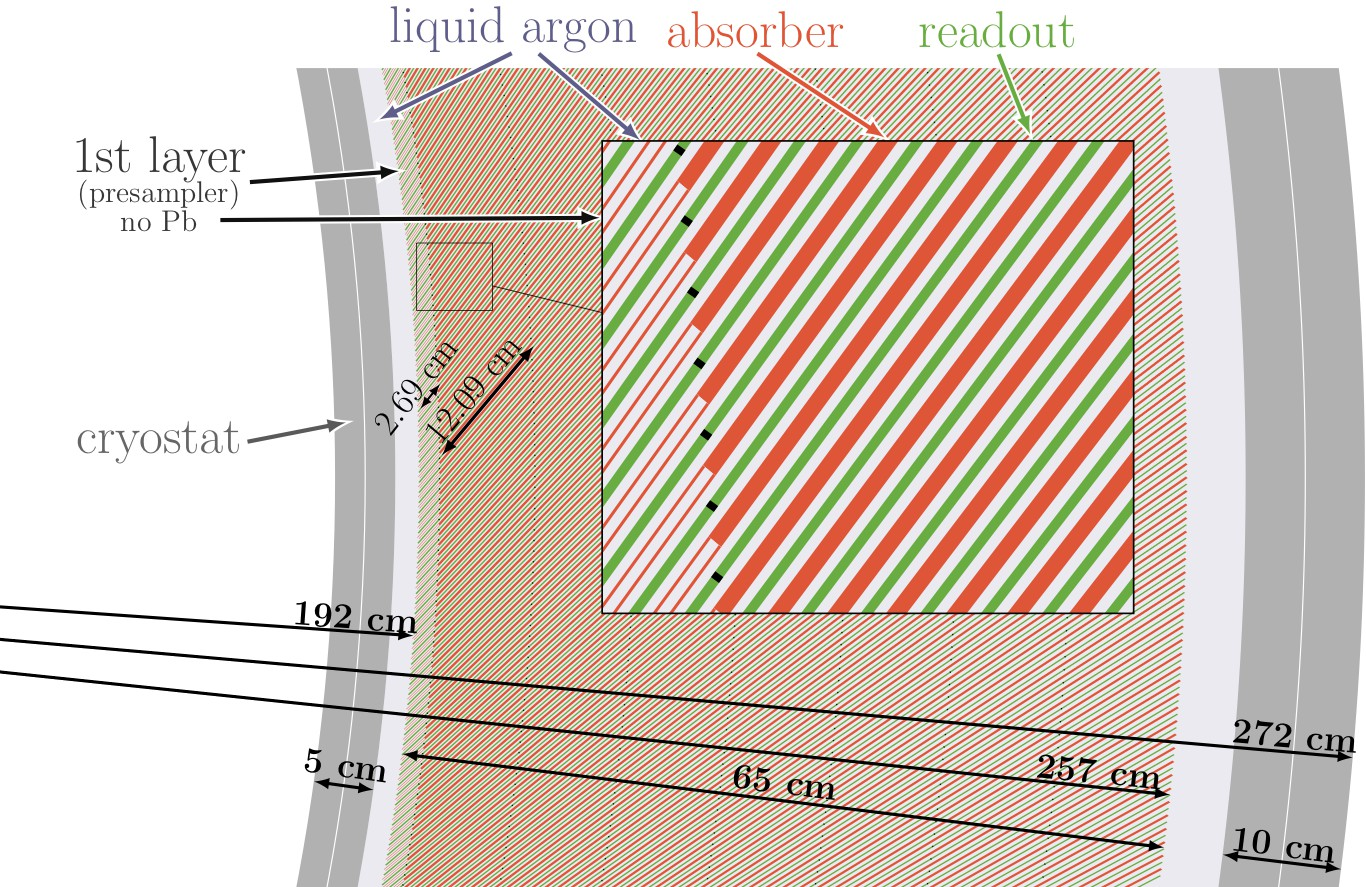
\includegraphics[width=0.49\linewidth]{figures/lar_calo_fcchh.png}
  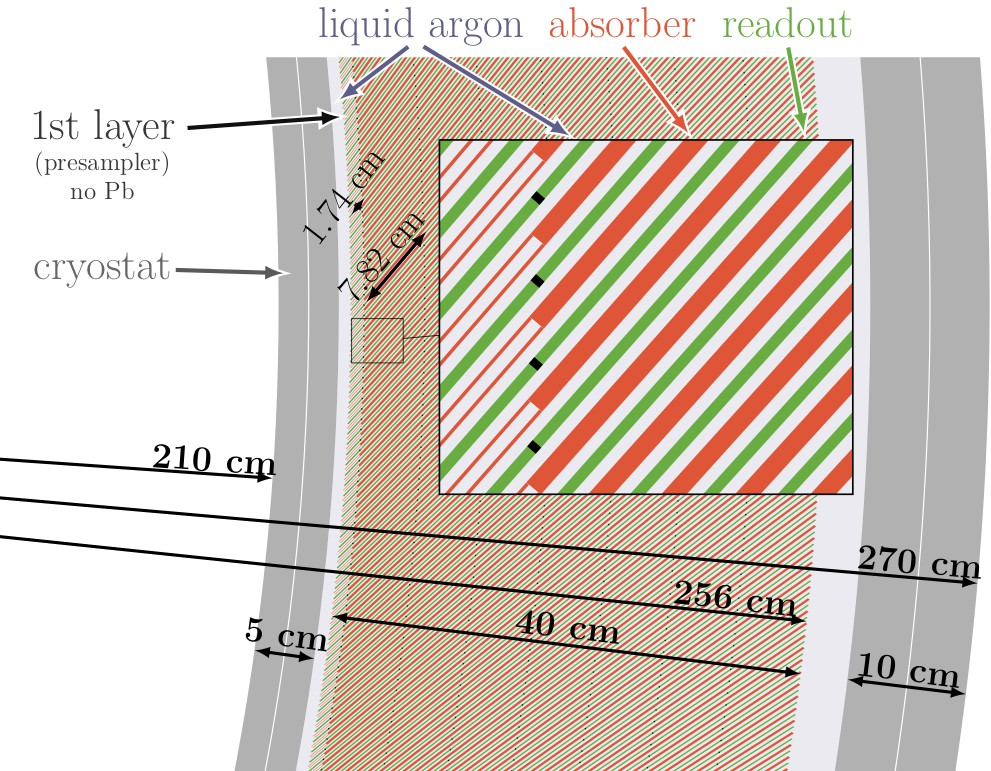
\includegraphics[width=0.49\linewidth]{figures/lar_calo_fccee.png}

  {\tiny
   \href{https://indico.cern.ch/event/969249/contributions/4086276/attachments/2132741/3591642/20201029_LAr_workingMeeting_Brieuc.pdf}
        {source: Brieuc François (CERN)}}
\end{frame}


% ---------------------------------------------------------------------------- %
\section{Location of energy deposits}

\begin{frame}
  \frametitle{FCC-hh: Energy deposits}

  \begin{itemize}
    \item FCC-hh, electron, 50 GeV, $\theta = \pi/2$
    \item Energy deposited in front cryostat and in the calorimeter
  \end{itemize}

  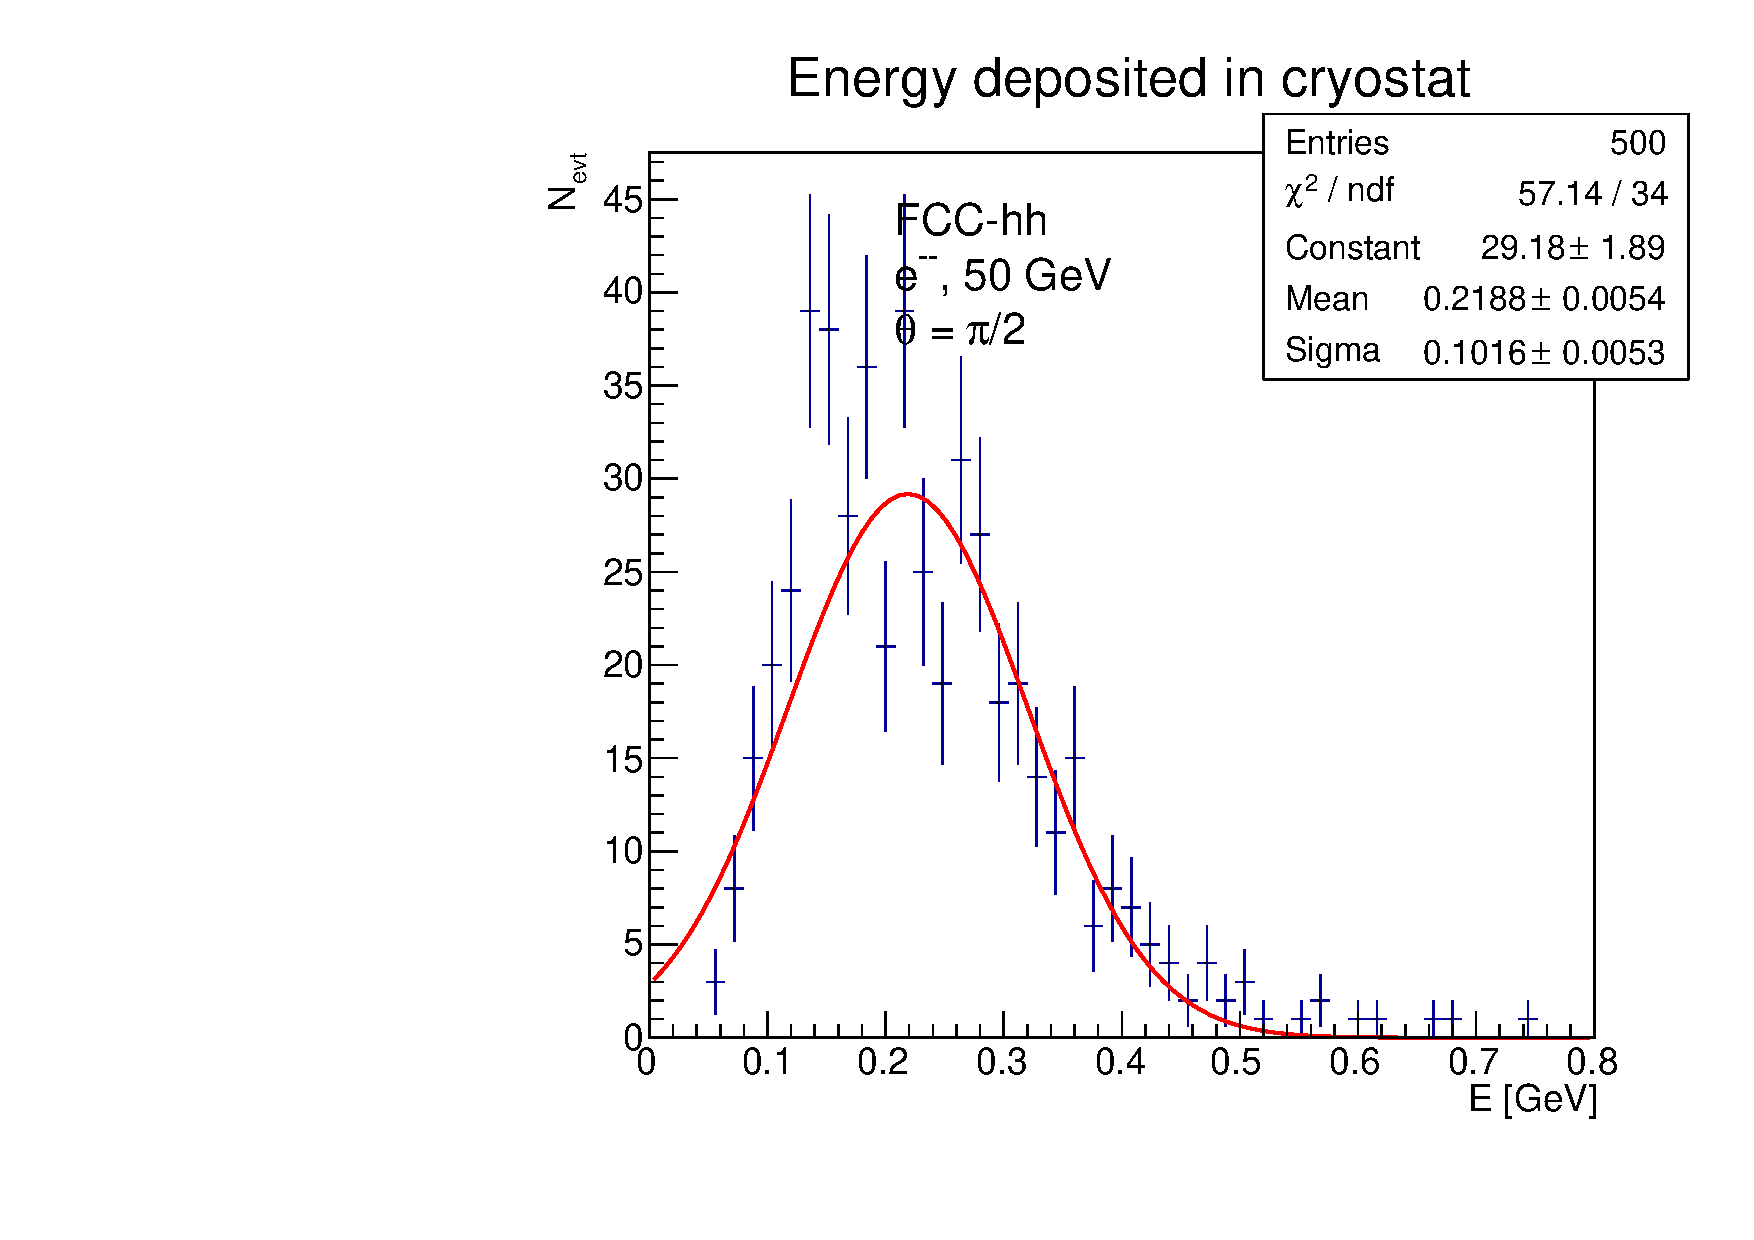
\includegraphics[width=0.49\linewidth]{figures/energy_fcchh/energyInCryo.pdf}
  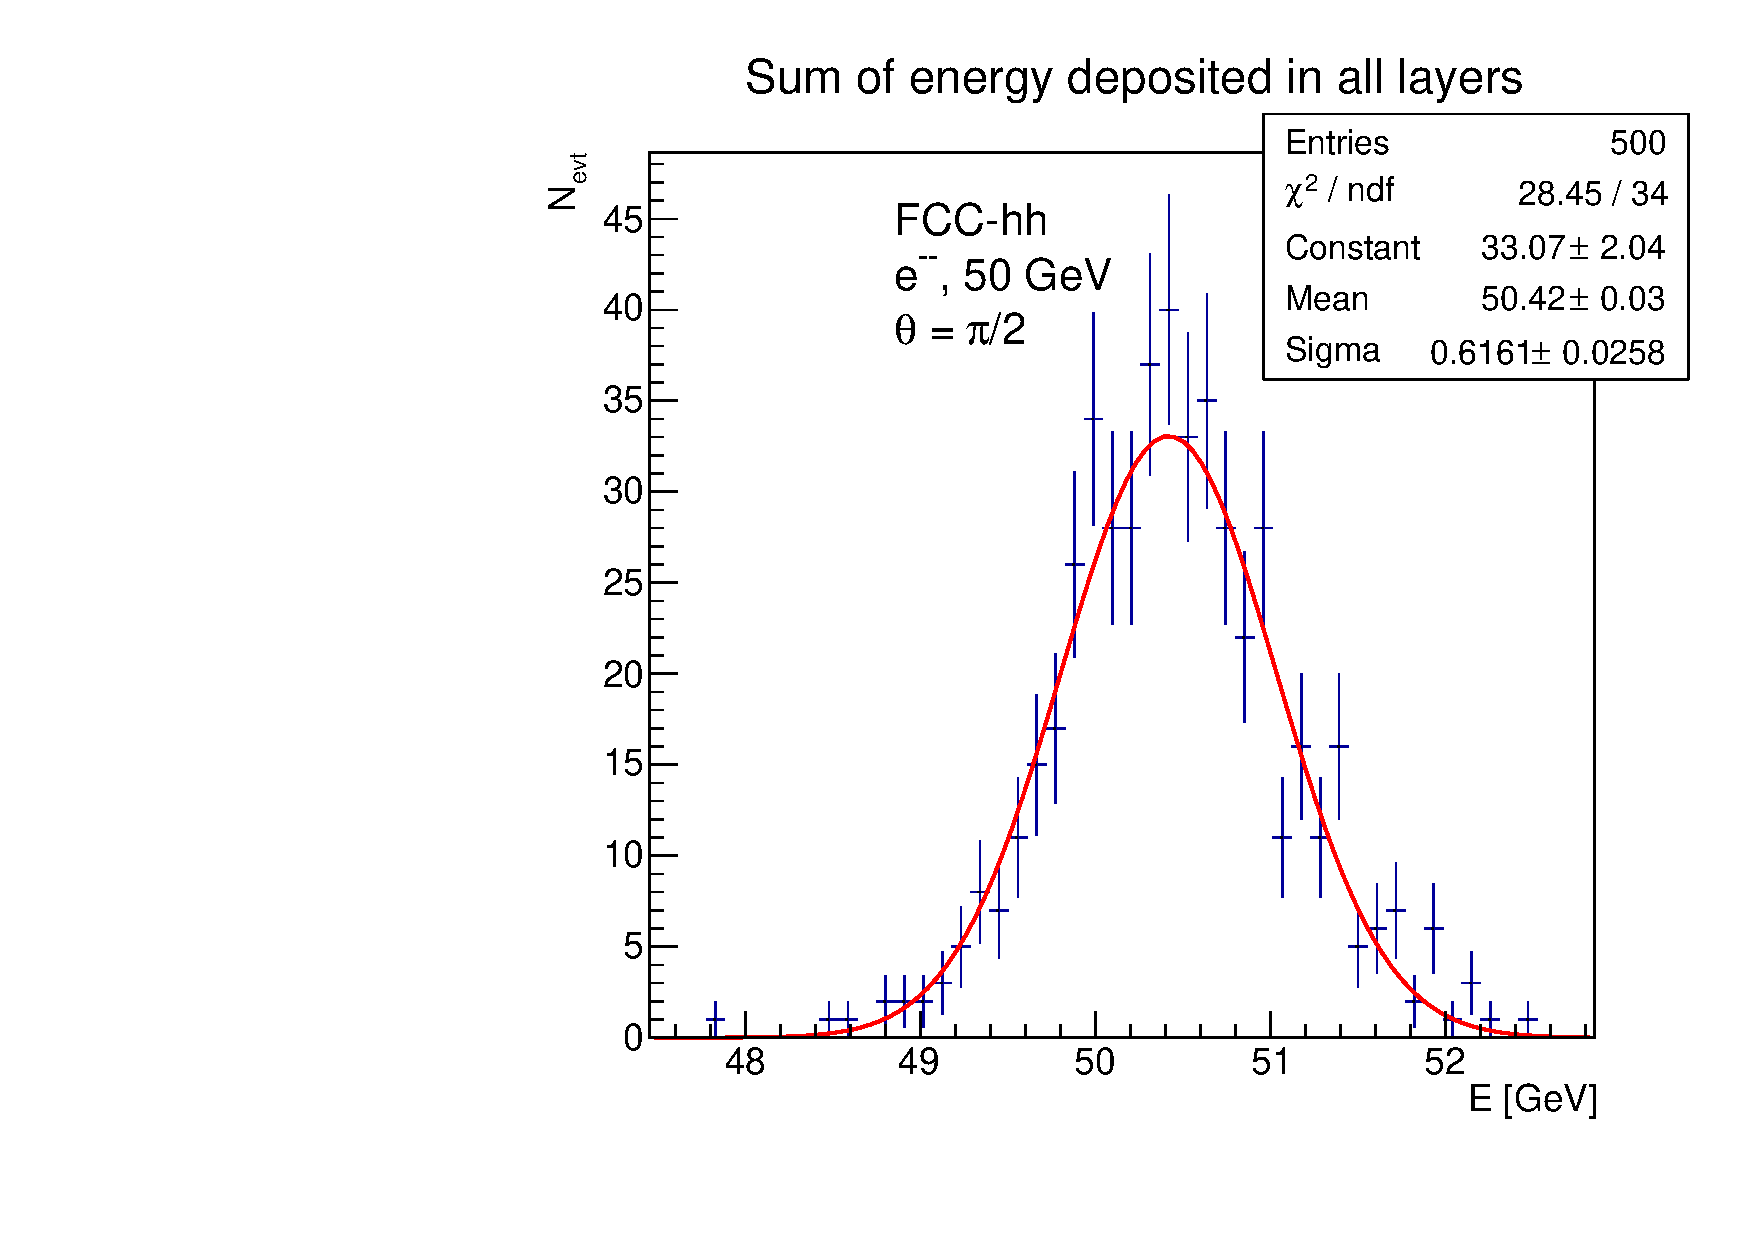
\includegraphics[width=0.49\linewidth]{figures/energy_fcchh/sumEinLayers.pdf}
\end{frame}

\begin{frame}
  \frametitle{FCC-hh: Energy deposits}

  \centering
  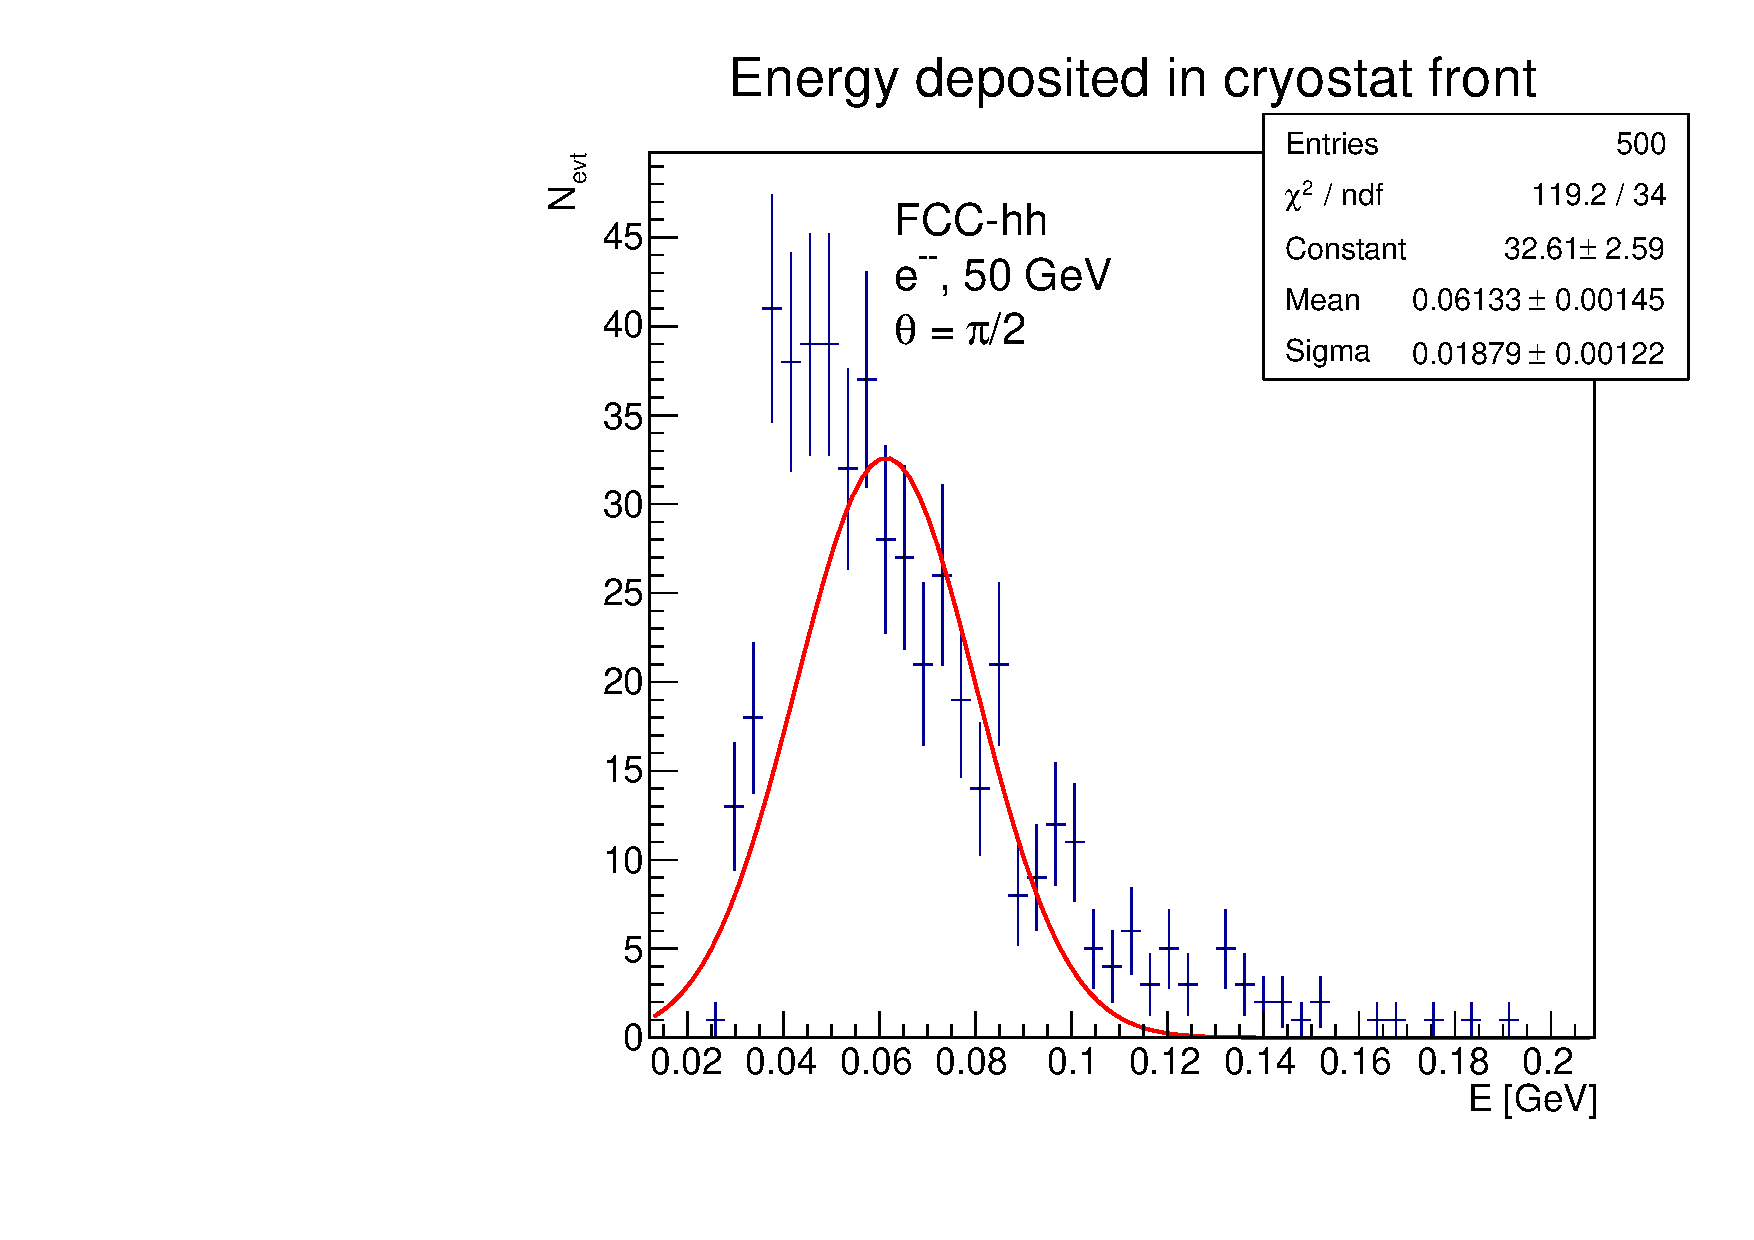
\includegraphics[width=0.39\linewidth]{figures/energy_fcchh/energyInCryoFront.pdf}
  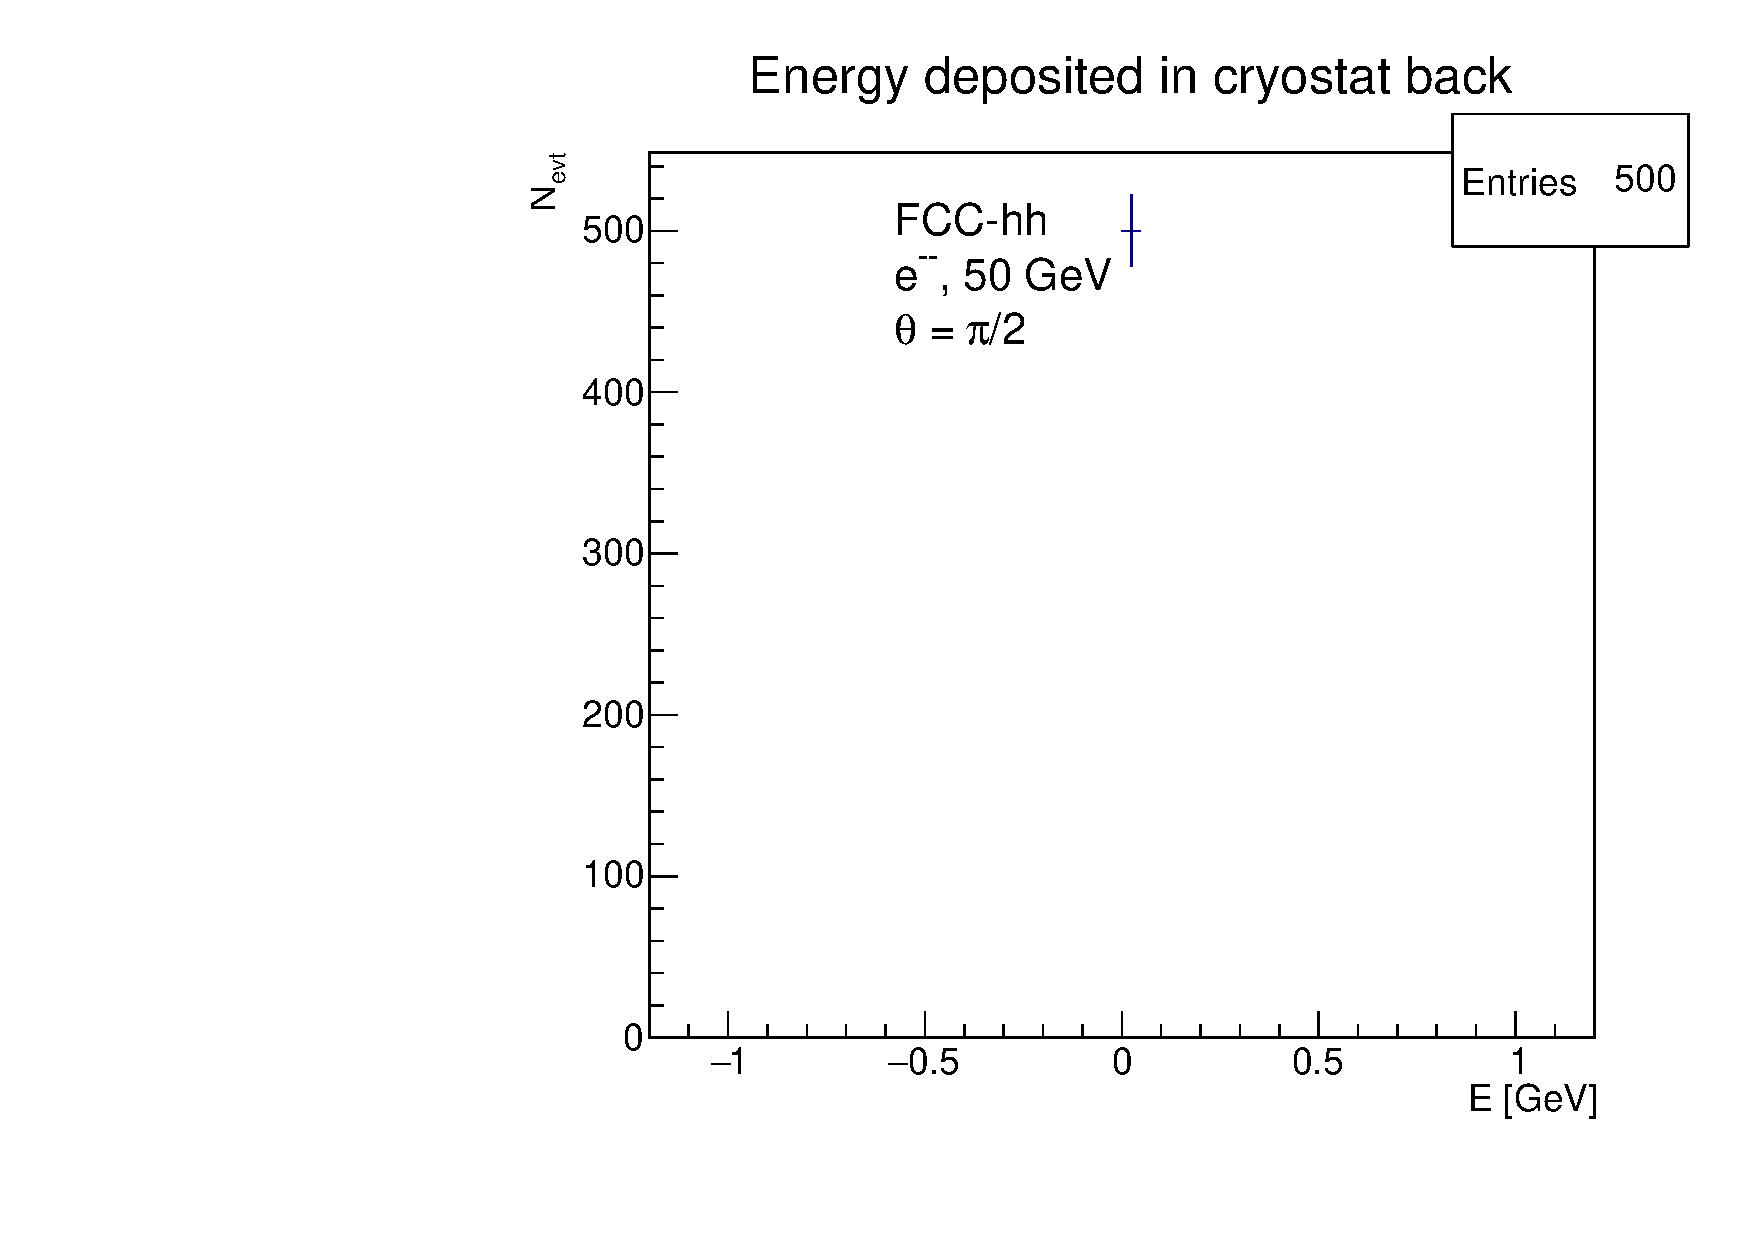
\includegraphics[width=0.39\linewidth]{figures/energy_fcchh/energyInCryoBack.pdf}
  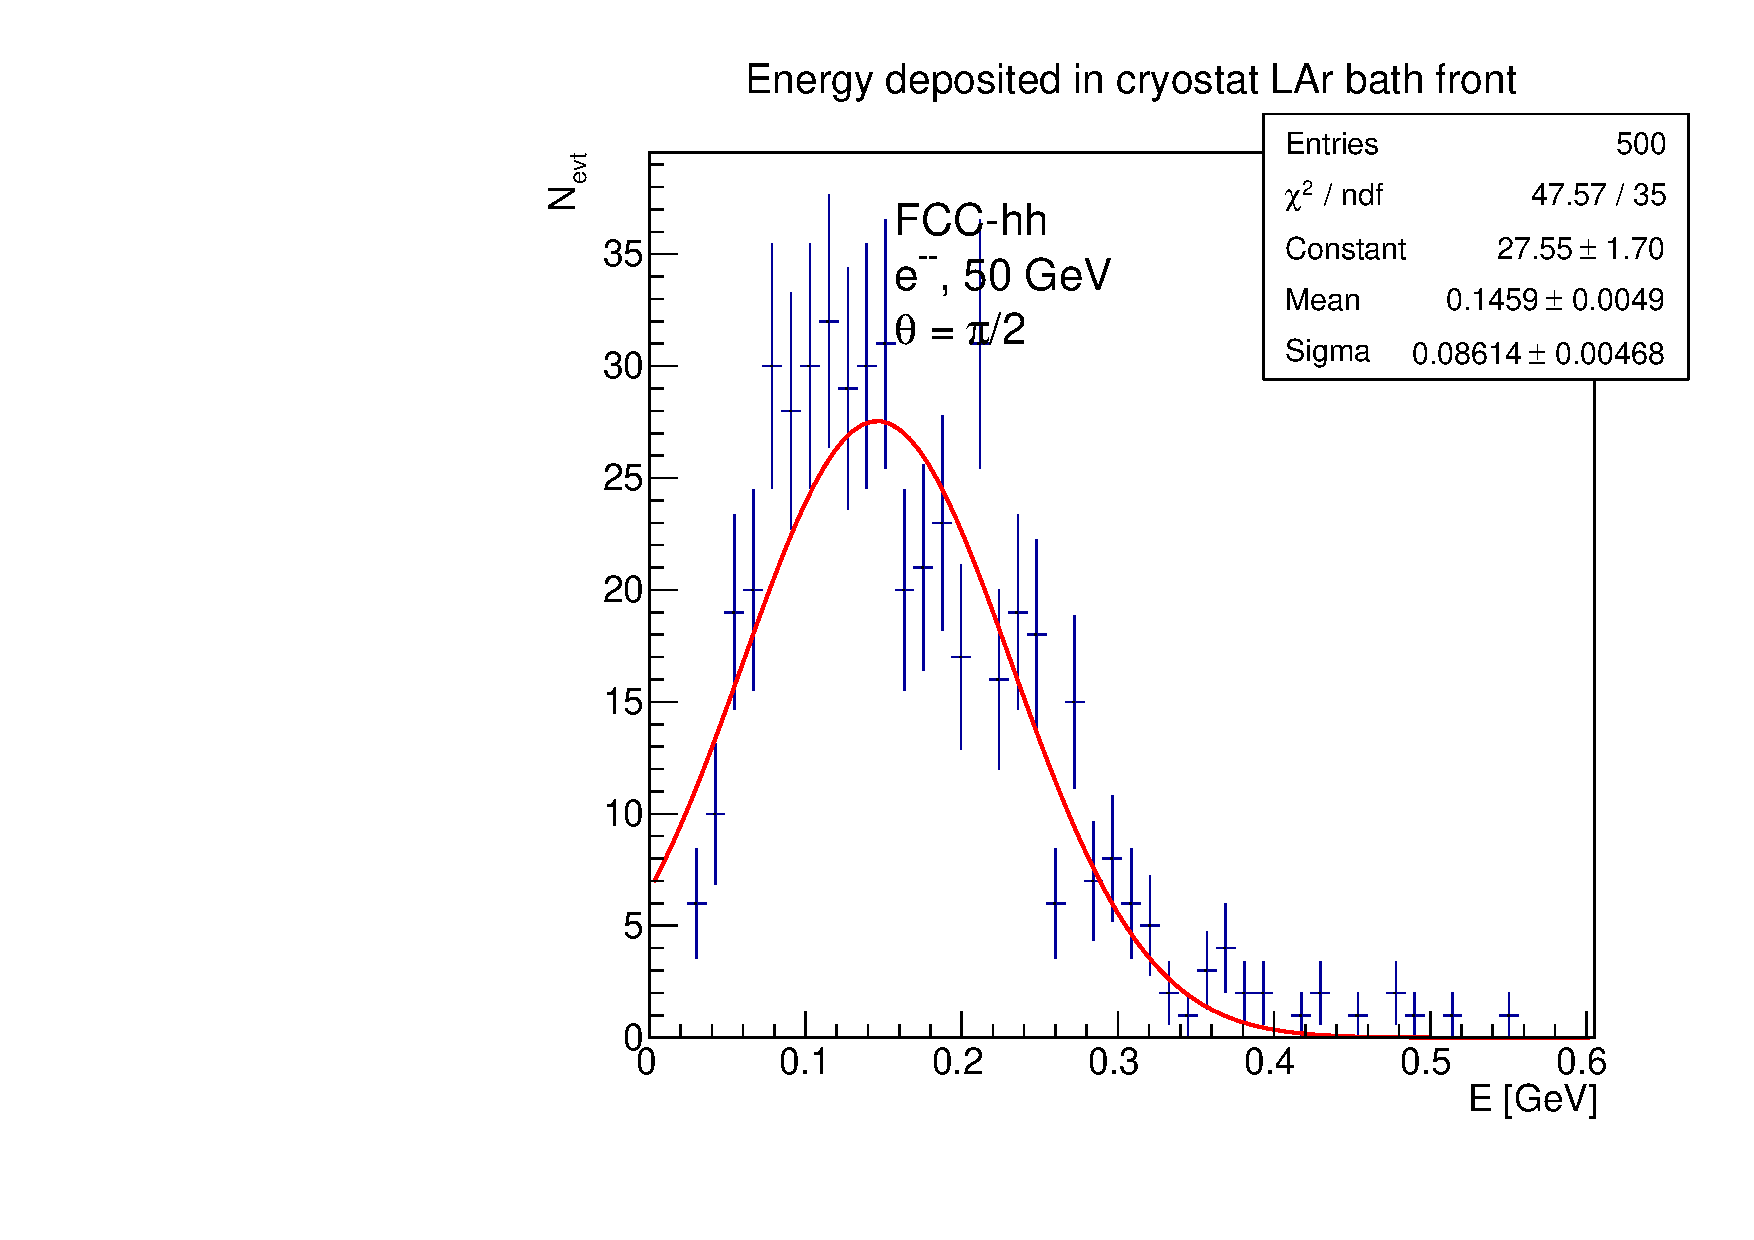
\includegraphics[width=0.39\linewidth]{figures/energy_fcchh/energyInCryoLArBathFront.pdf}
  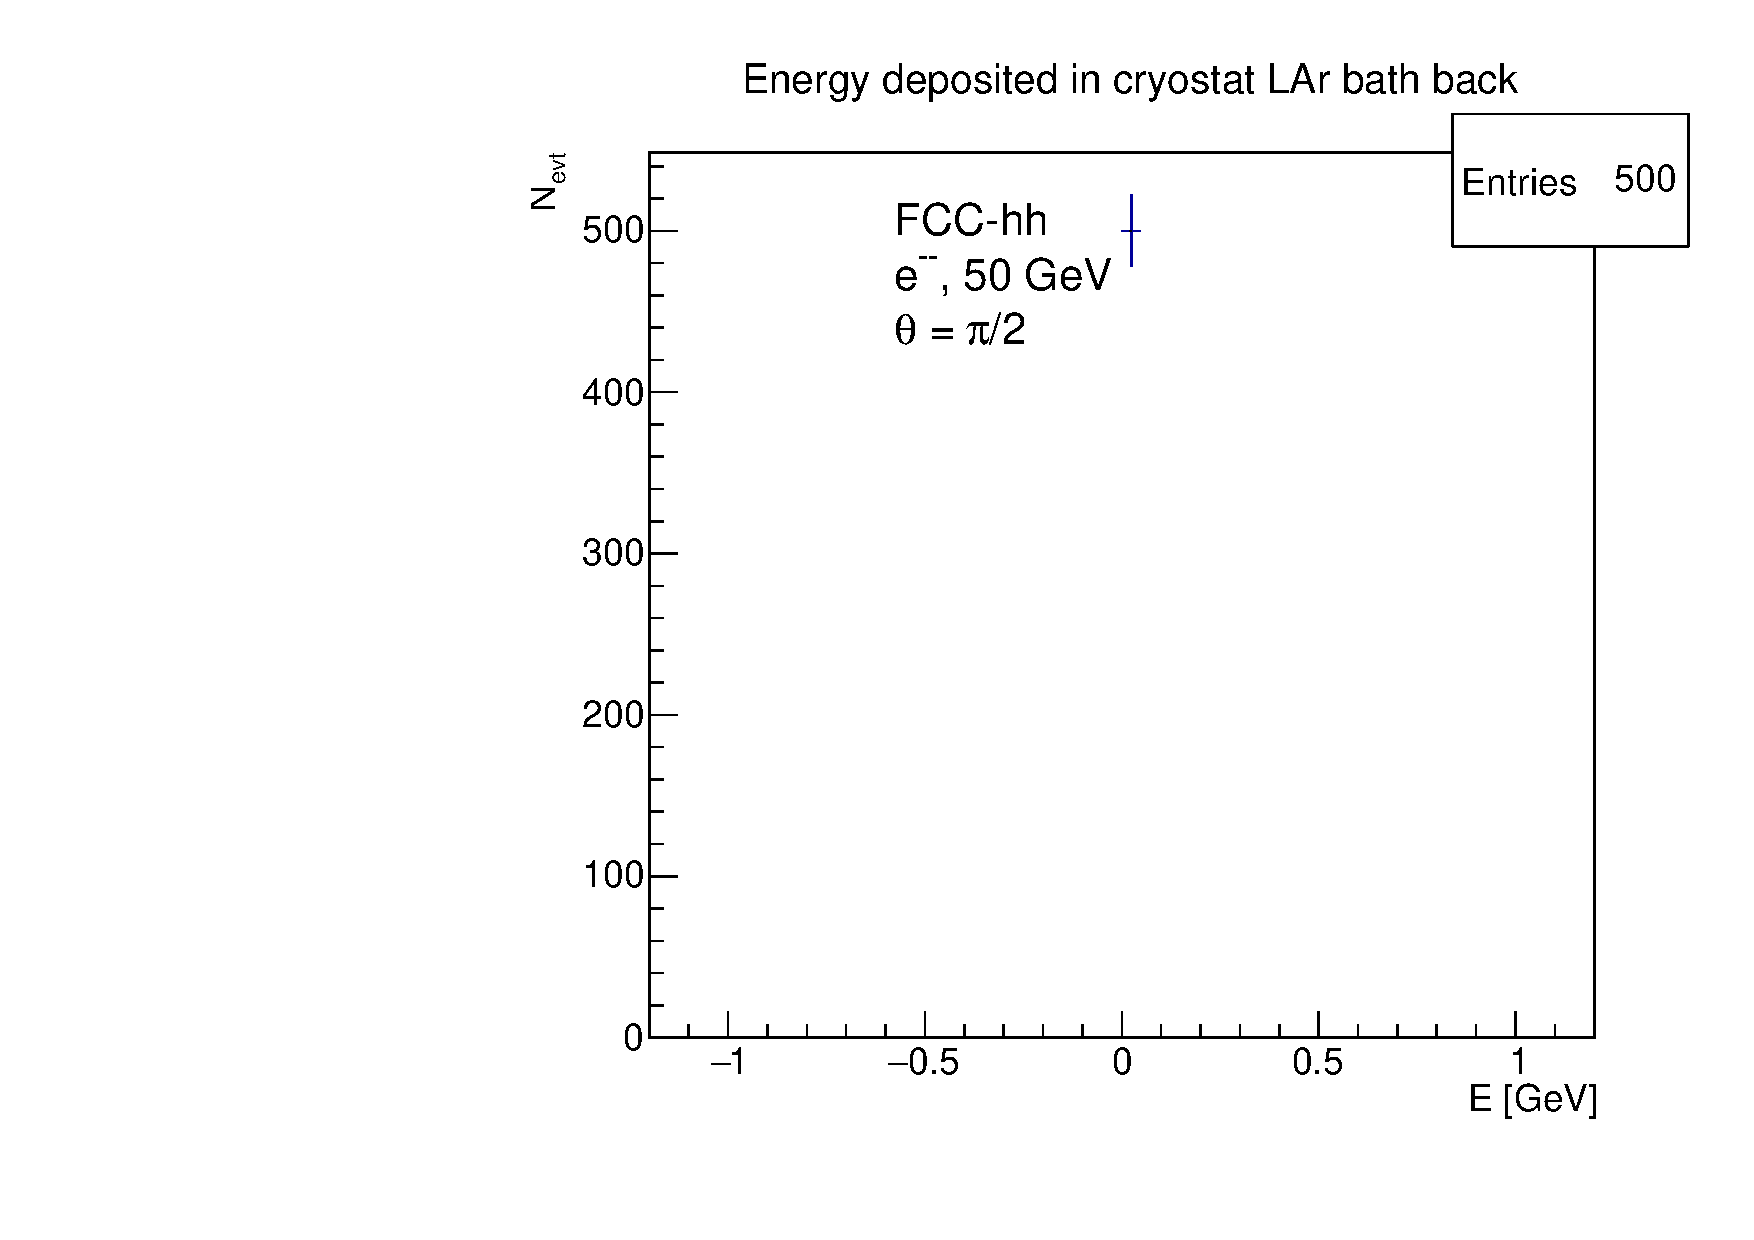
\includegraphics[width=0.39\linewidth]{figures/energy_fcchh/energyInCryoLArBathBack.pdf}
\end{frame}

\begin{frame}
  \frametitle{FCC-ee: Energy deposits}

  \begin{itemize}
    \item FCC-ee, electron, 50 GeV, $\theta = \pi/2$
    \item Energy deposited not only in front cryostat and in the
          calorimeter, \redtext{but in the back cryostat as well}
  \end{itemize}

  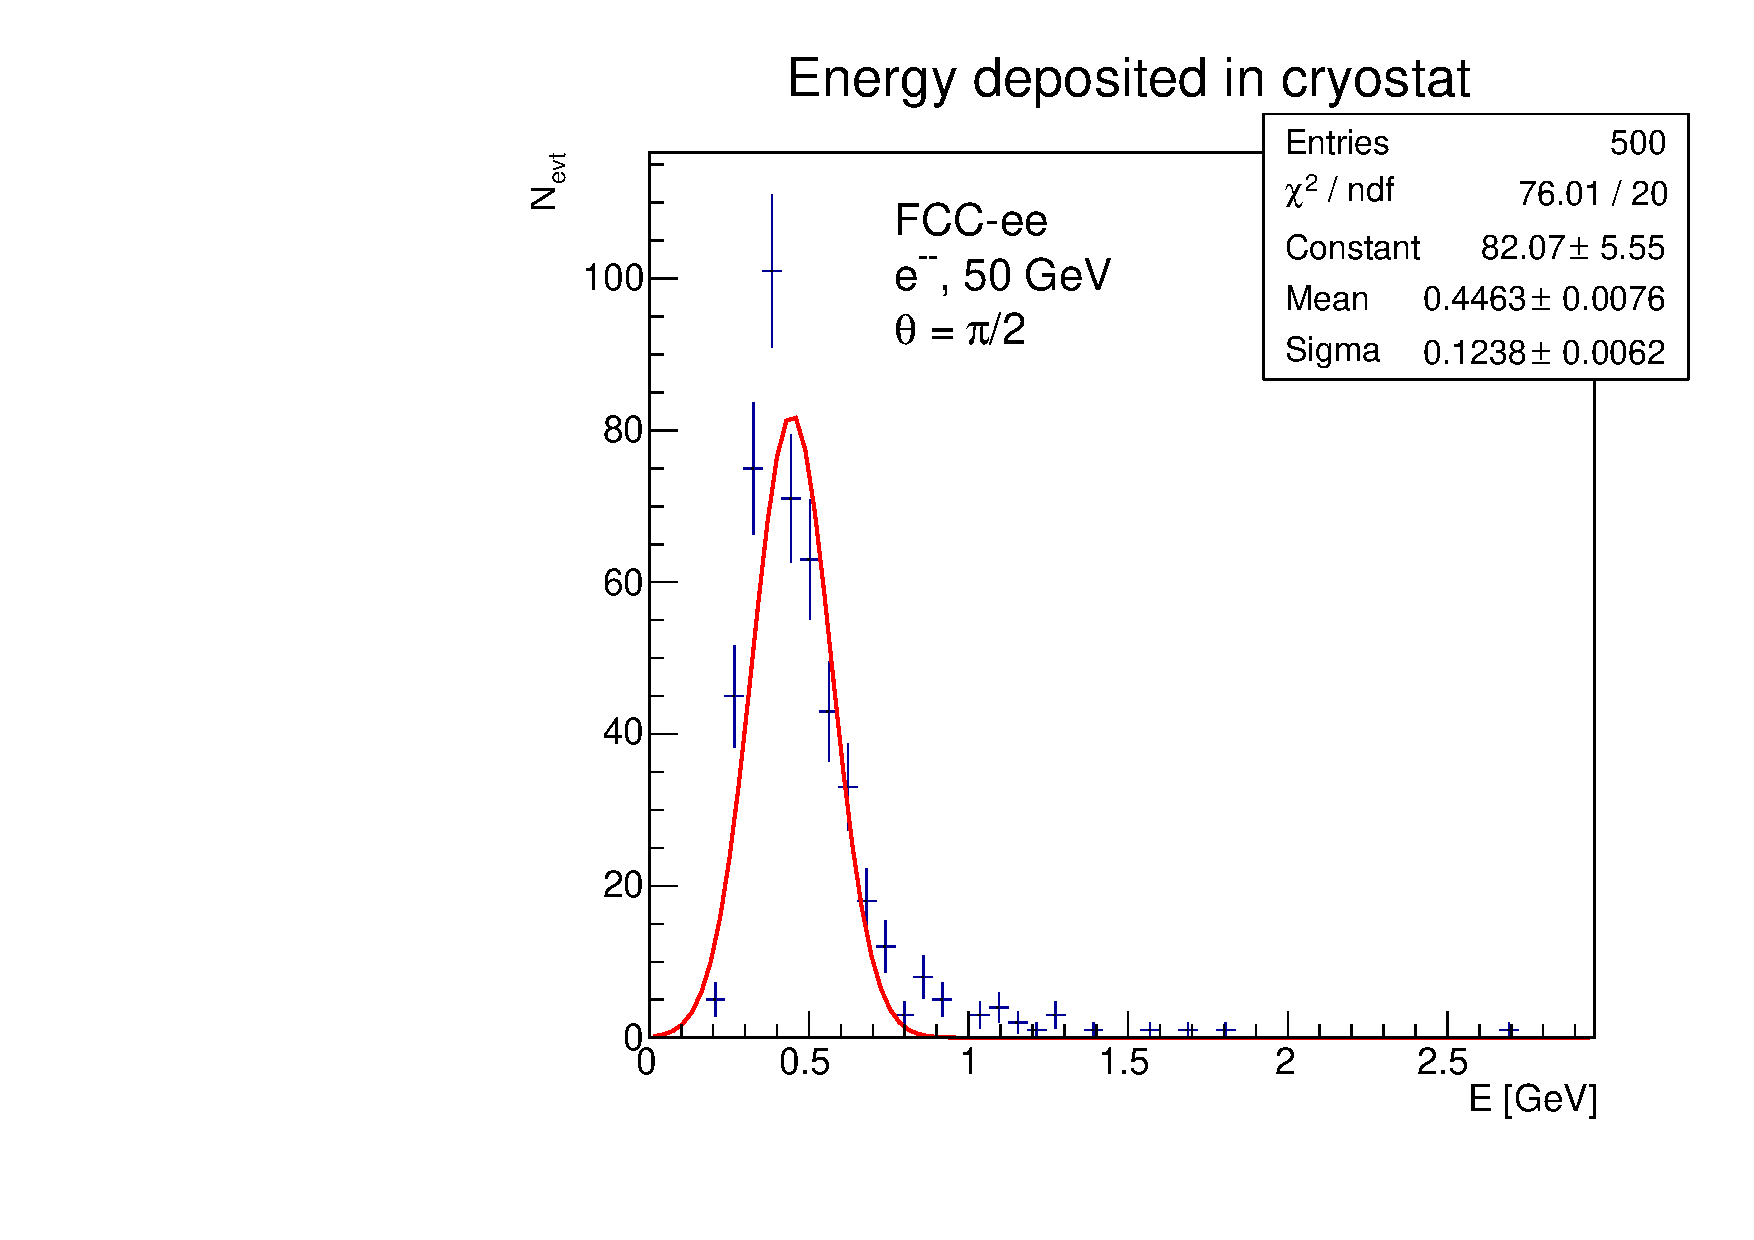
\includegraphics[width=0.49\linewidth]{figures/energy_fccee/energyInCryo.pdf}
  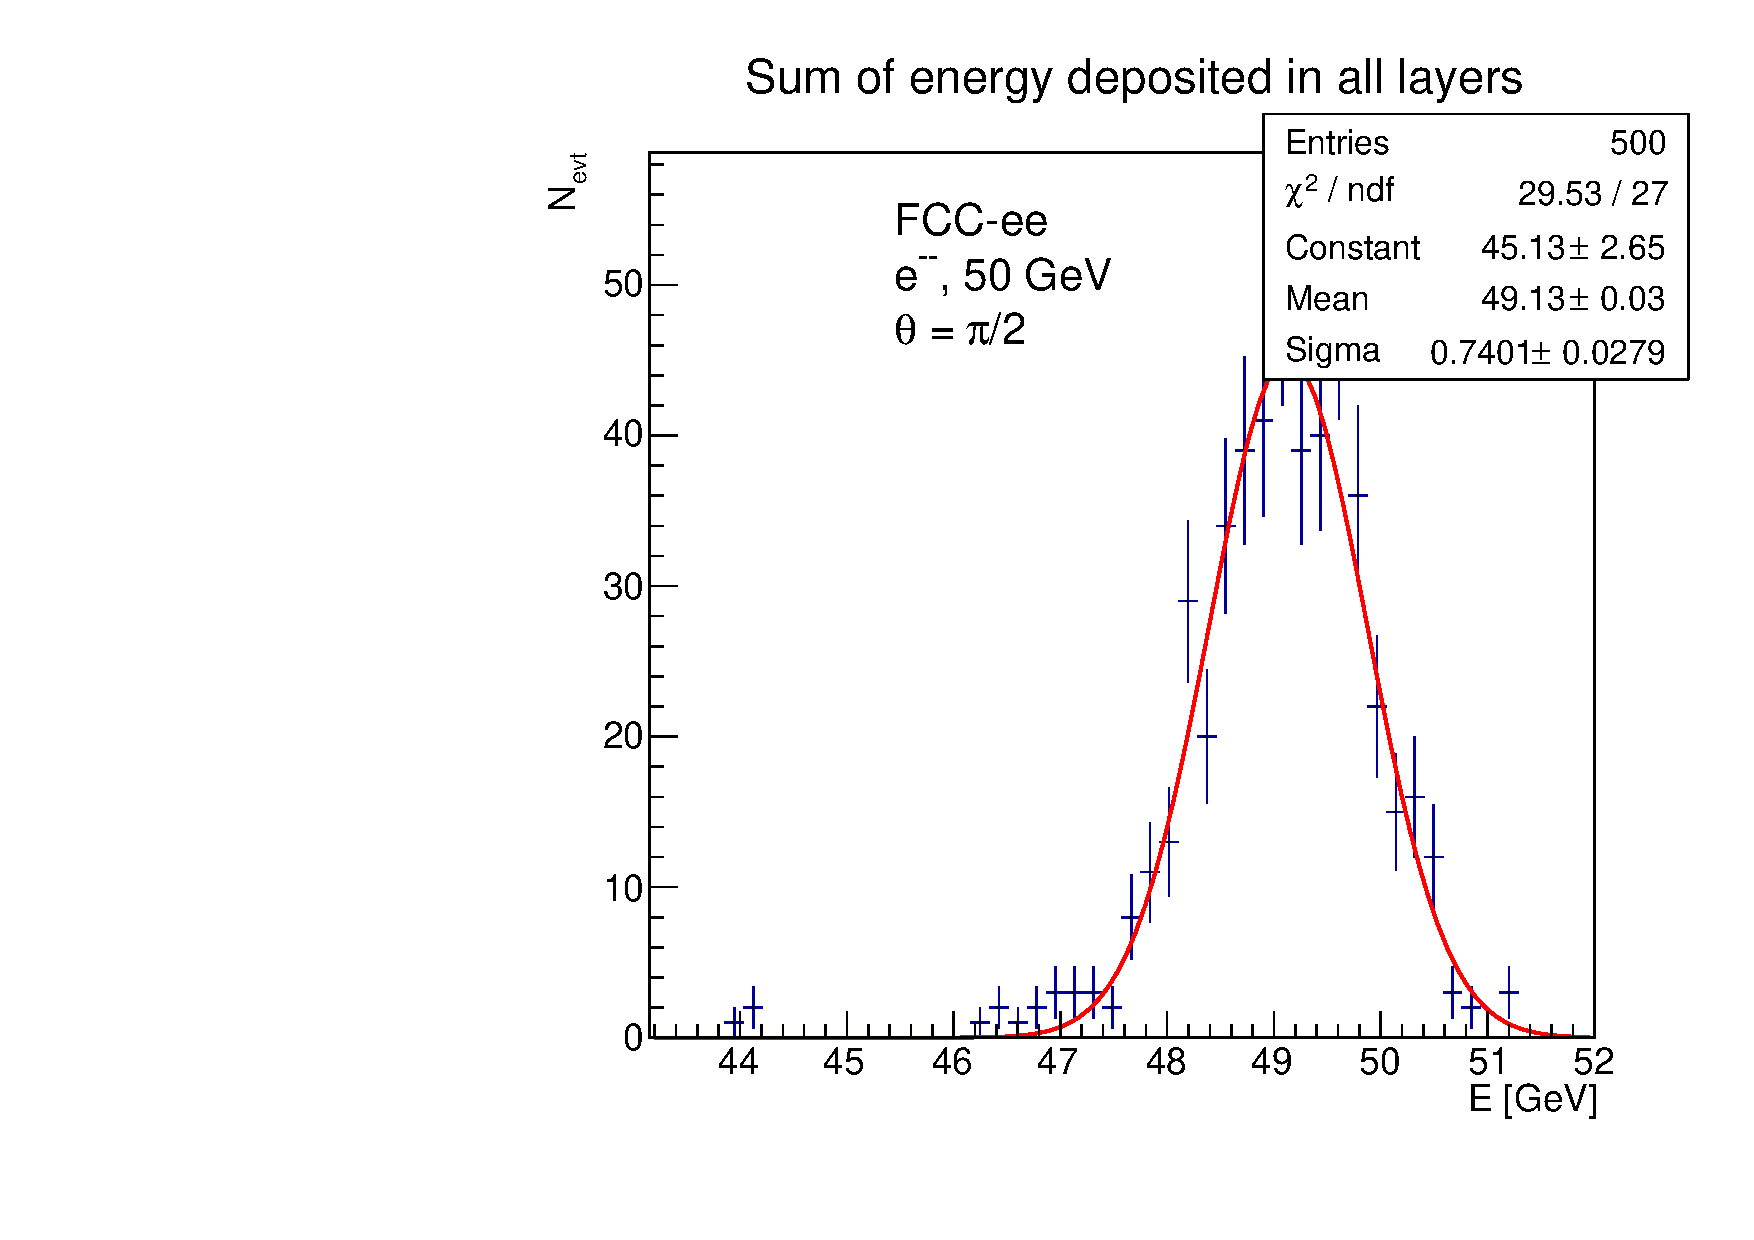
\includegraphics[width=0.49\linewidth]{figures/energy_fccee/sumEinLayers.pdf}
\end{frame}

\begin{frame}
  \frametitle{FCC-ee: Energy deposits}

  \centering
  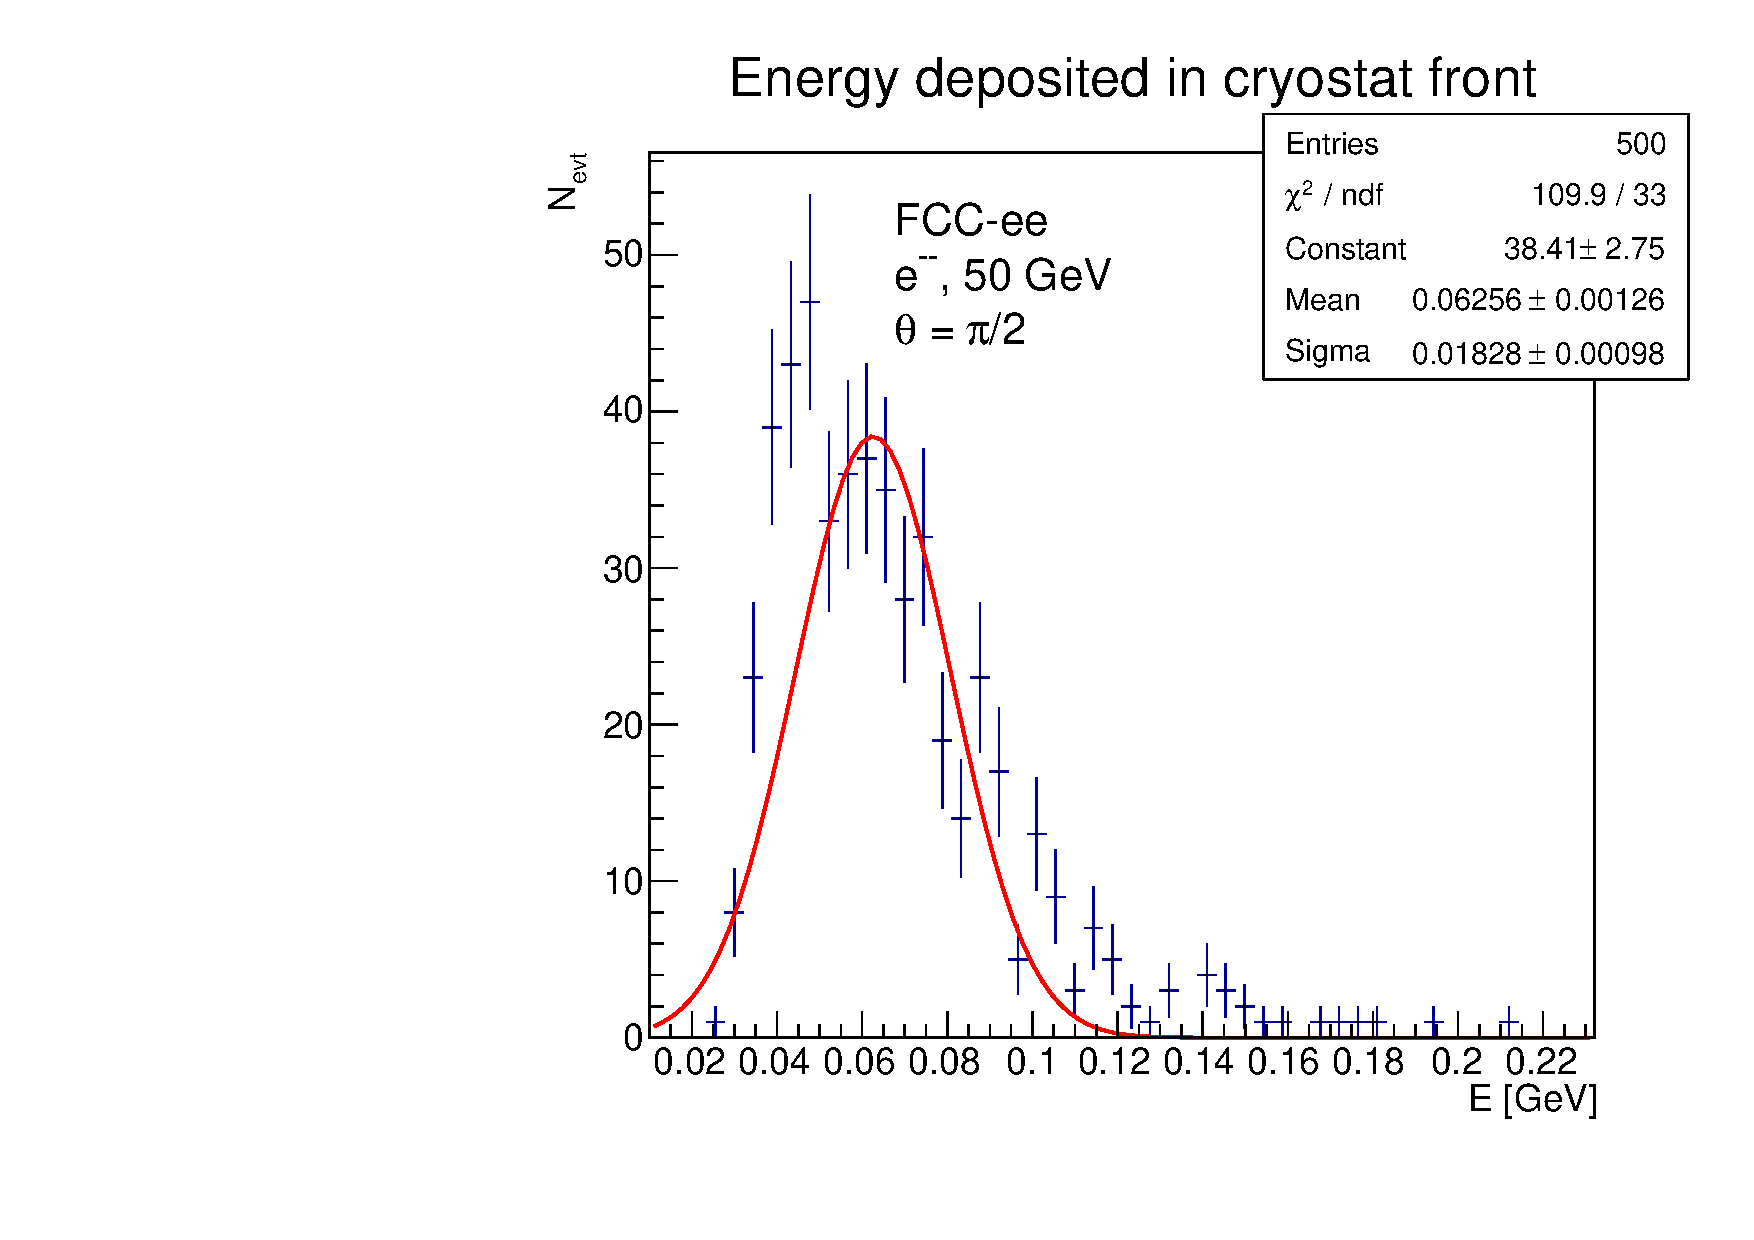
\includegraphics[width=0.39\linewidth]{figures/energy_fccee/energyInCryoFront.pdf}
  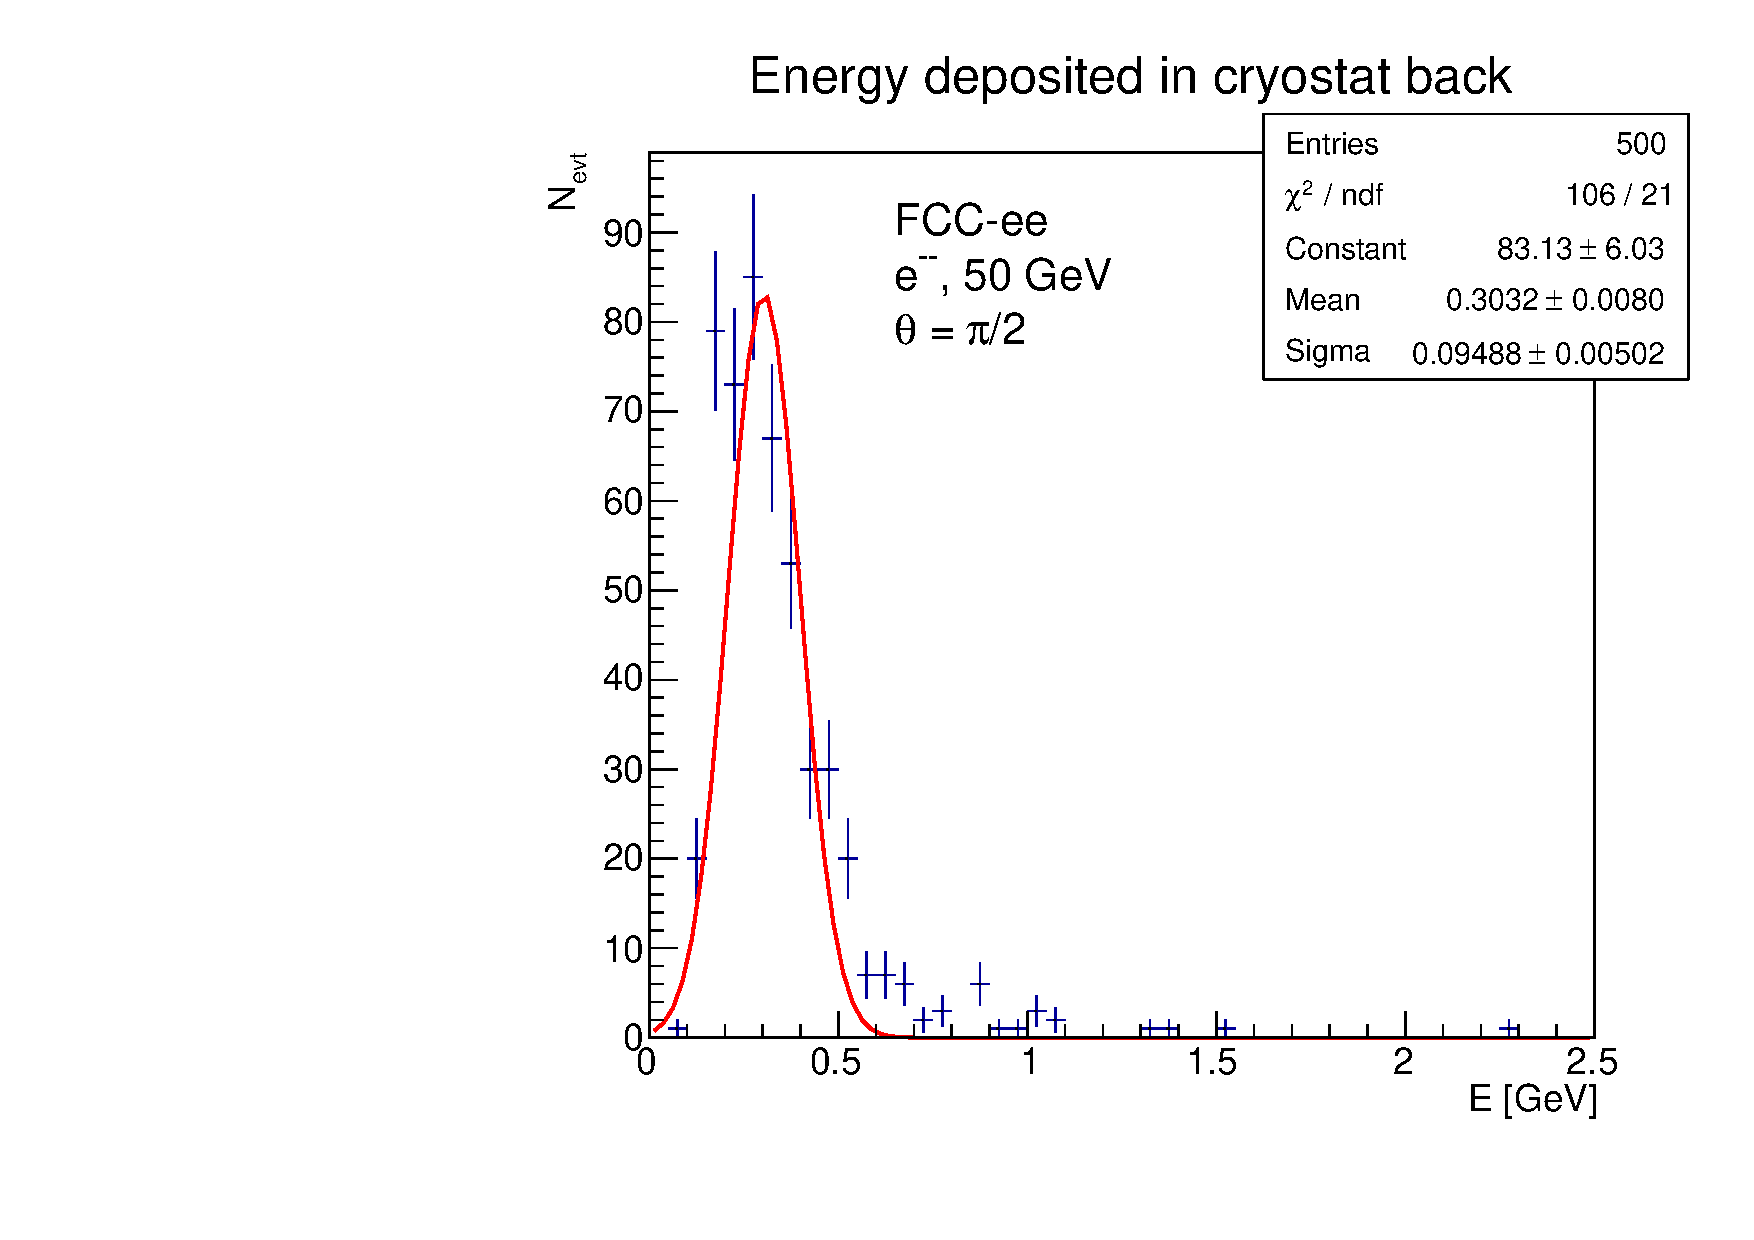
\includegraphics[width=0.39\linewidth]{figures/energy_fccee/energyInCryoBack.pdf}
  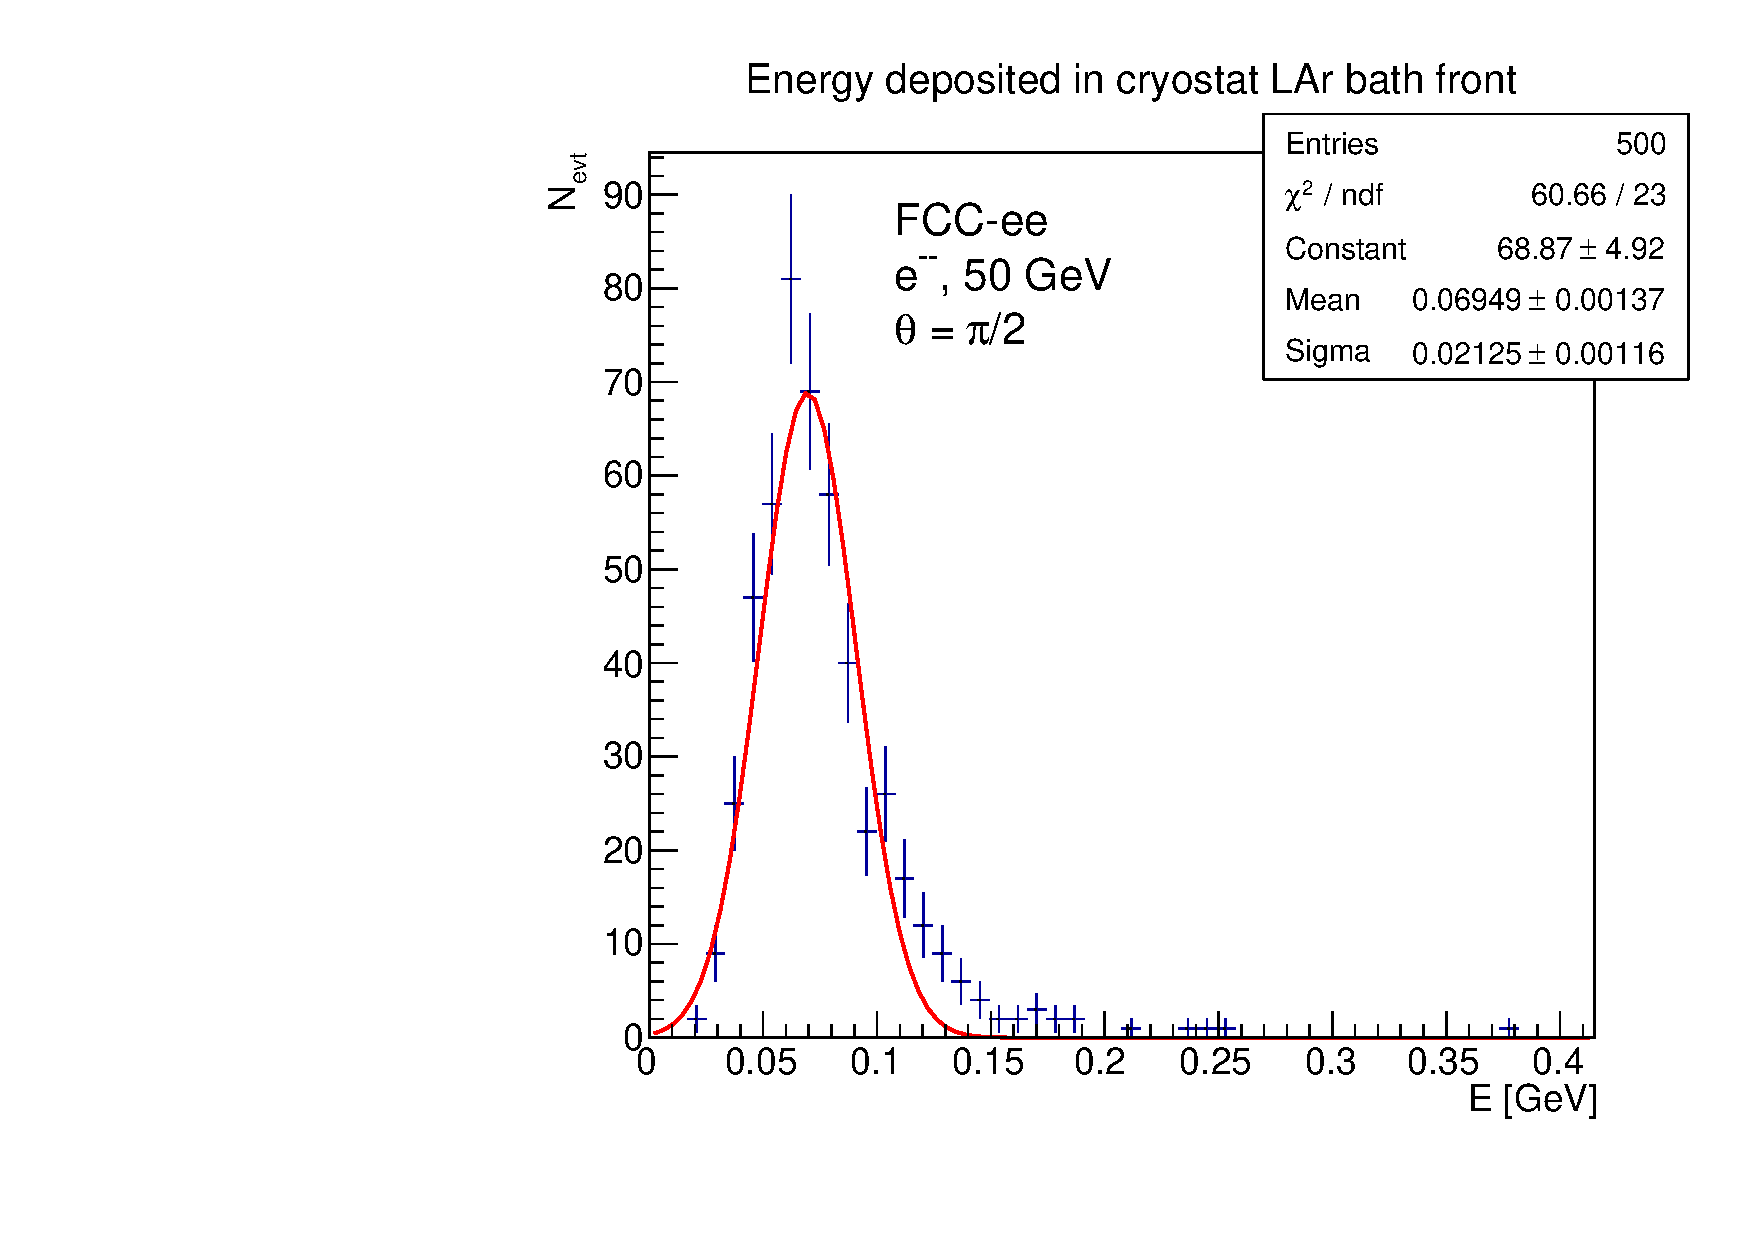
\includegraphics[width=0.39\linewidth]{figures/energy_fccee/energyInCryoLArBathFront.pdf}
  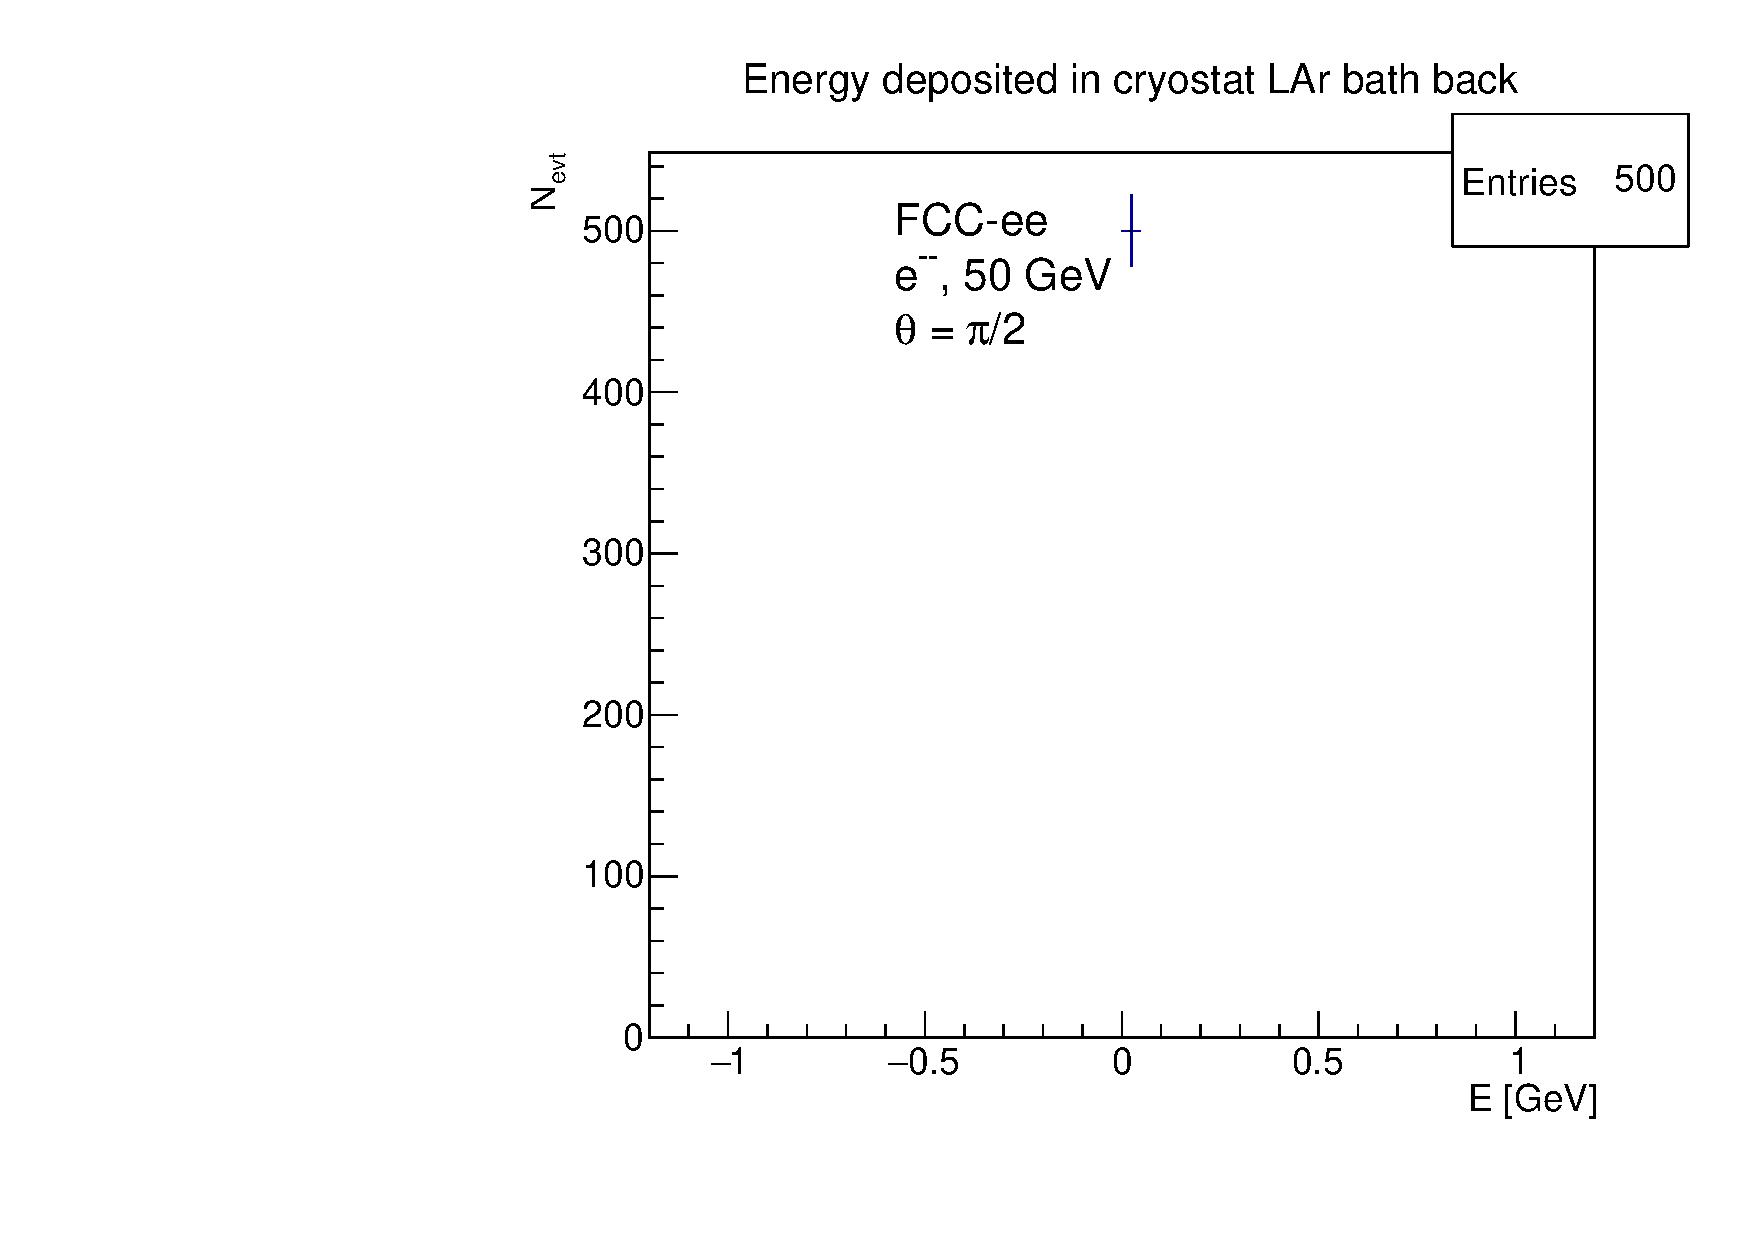
\includegraphics[width=0.39\linewidth]{figures/energy_fccee/energyInCryoLArBathBack.pdf}
\end{frame}


% ---------------------------------------------------------------------------- %
\section{Upstream Correction}

\begin{frame}
  \frametitle{Upstream Correction at FCC-hh Calorimeter}

  \redtext{FCC-hh} parametrization:

  \begin{equation*}
    E = E_\text{upstream} + E_\text{cluster}
  \end{equation*}

  \begin{equation*}
  E_\text{upstream} = P_0(E_\text{cluster}, |\eta|) +
                      P_1(E_\text{cluster}, |\eta|) \cdot E_\text{firstLayer}
  \end{equation*}

  \begin{equation*}
    P_0 = P_{00}(|\eta|) + P_{01}(|\eta|) \cdot E_{cluster}  \qquad
    P_1 = P_{10}(|\eta|) + \frac{P_{11}(|\eta|)}{\sqrt{E_{cluster}}}
  \end{equation*}

  \begin{center}
    No $\eta$ dependence
  \end{center}
\end{frame}

\begin{frame}
  \frametitle{Upstream Correction FCC-hh vs. FCC-ee}

  \begin{itemize}
    \item Energy deposited in first layer correlates with upstream energy for
          both FCC-hh and FCC-ee
    \item Smaller upstream energy $\rightarrow$ thinner front LAr bath
          \begin{itemize}
            \item 90~mm $\rightarrow$ 20~mm
          \end{itemize}
    \item Smaller energy in first layer $\rightarrow$ thinner first layer
          (presampler)
          \begin{itemize}
            \item plate length 2.69~cm $\rightarrow$ 1.74~cm
          \end{itemize}
  \end{itemize}

  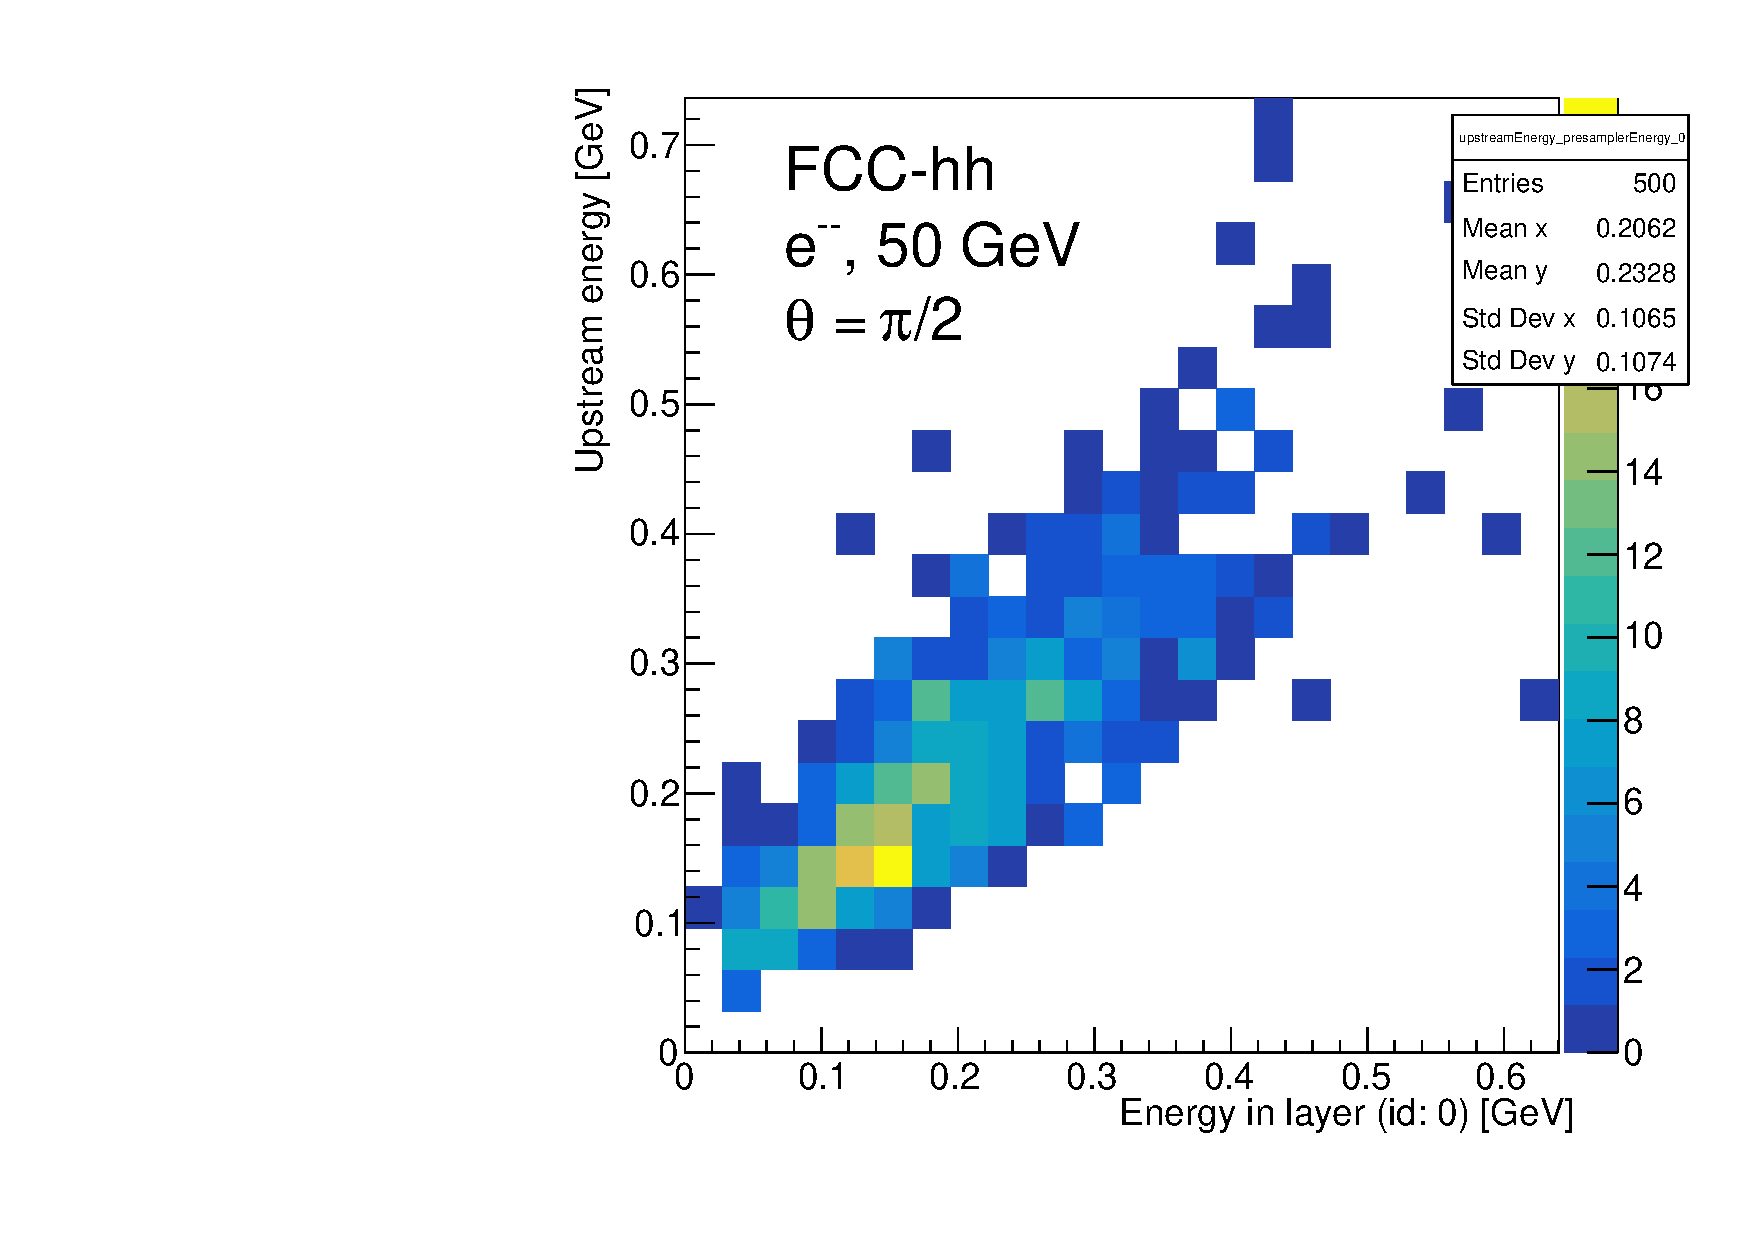
\includegraphics[width=0.49\linewidth]{figures/fcchh_hist_upstream_vs_first_layer_90deg_50GeV.pdf}
  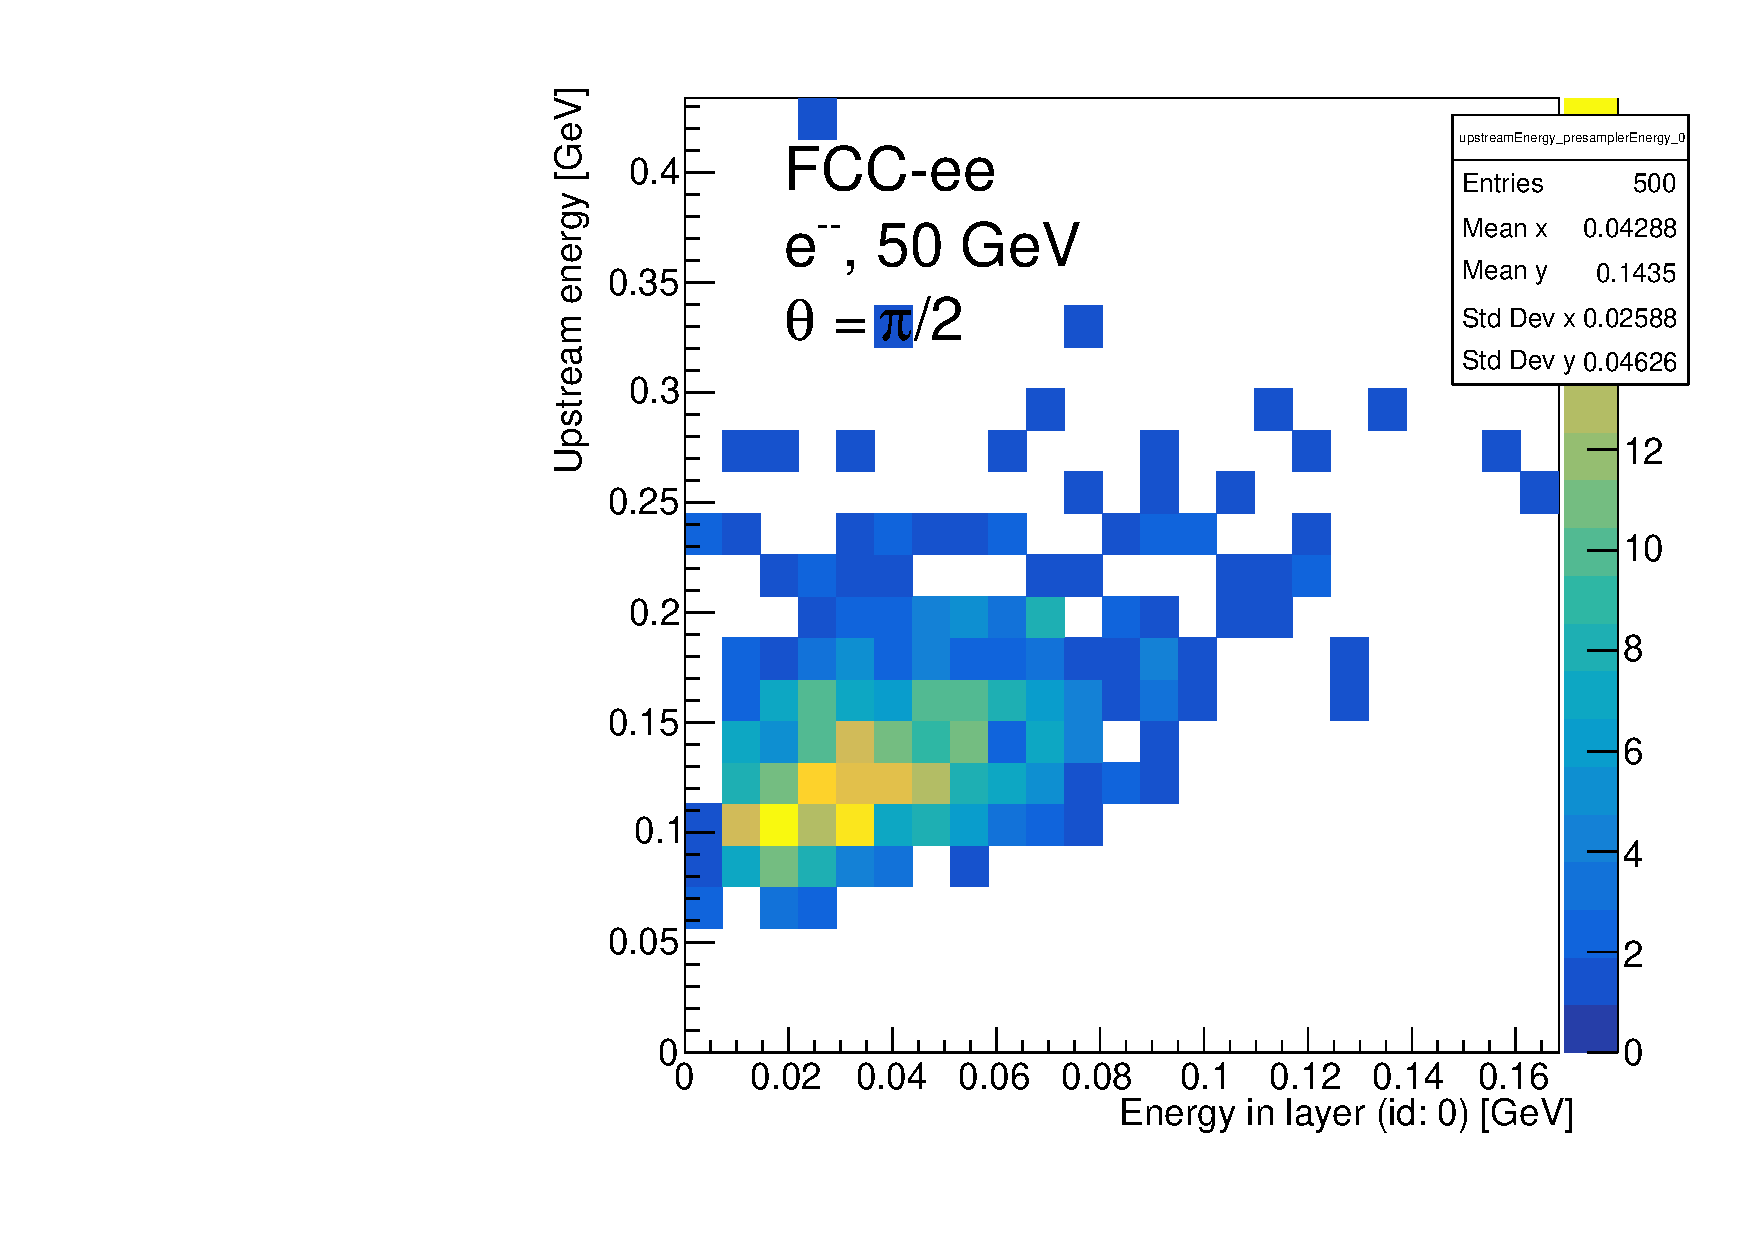
\includegraphics[width=0.49\linewidth]{figures/fccee_hist_upstream_vs_first_layer_90deg_50GeV.pdf}
\end{frame}

\begin{frame}
  \frametitle{Upstream Correction FCC-hh vs. FCC-ee}

  \begin{itemize}
    \item Energy deposited in first layer correlates with upstream energy for
          both FCC-hh and FCC-ee
    \item Smaller upstream energy $\rightarrow$ thinner front LAr bath
          \begin{itemize}
            \item 90~mm $\rightarrow$ 20~mm
          \end{itemize}
    \item Smaller energy in first layer $\rightarrow$ thinner first layer
          (presampler)
          \begin{itemize}
            \item plate length 2.69~cm $\rightarrow$ 1.74~cm
          \end{itemize}
  \end{itemize}

  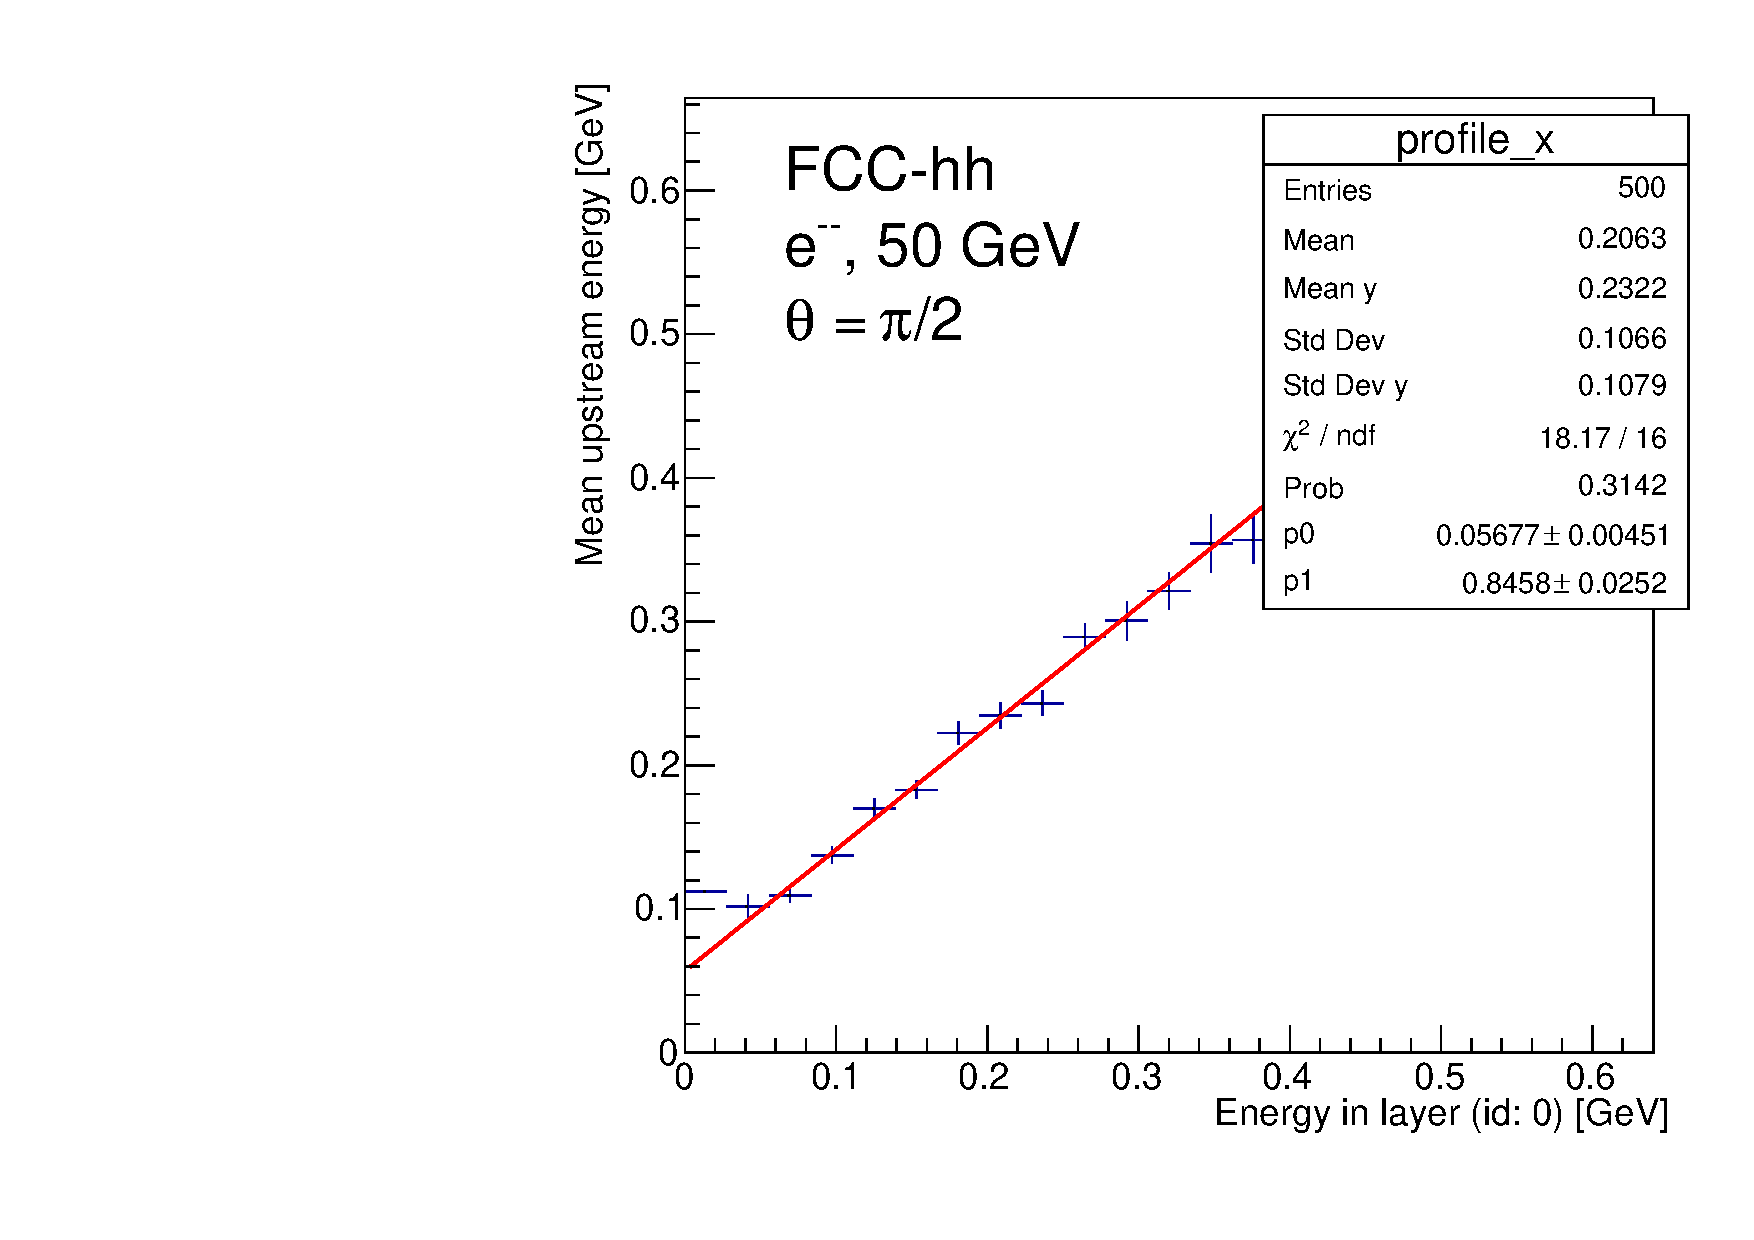
\includegraphics[width=0.49\linewidth]{figures/fcchh_profile_upstream_vs_first_layer_90deg_50GeV.pdf}
  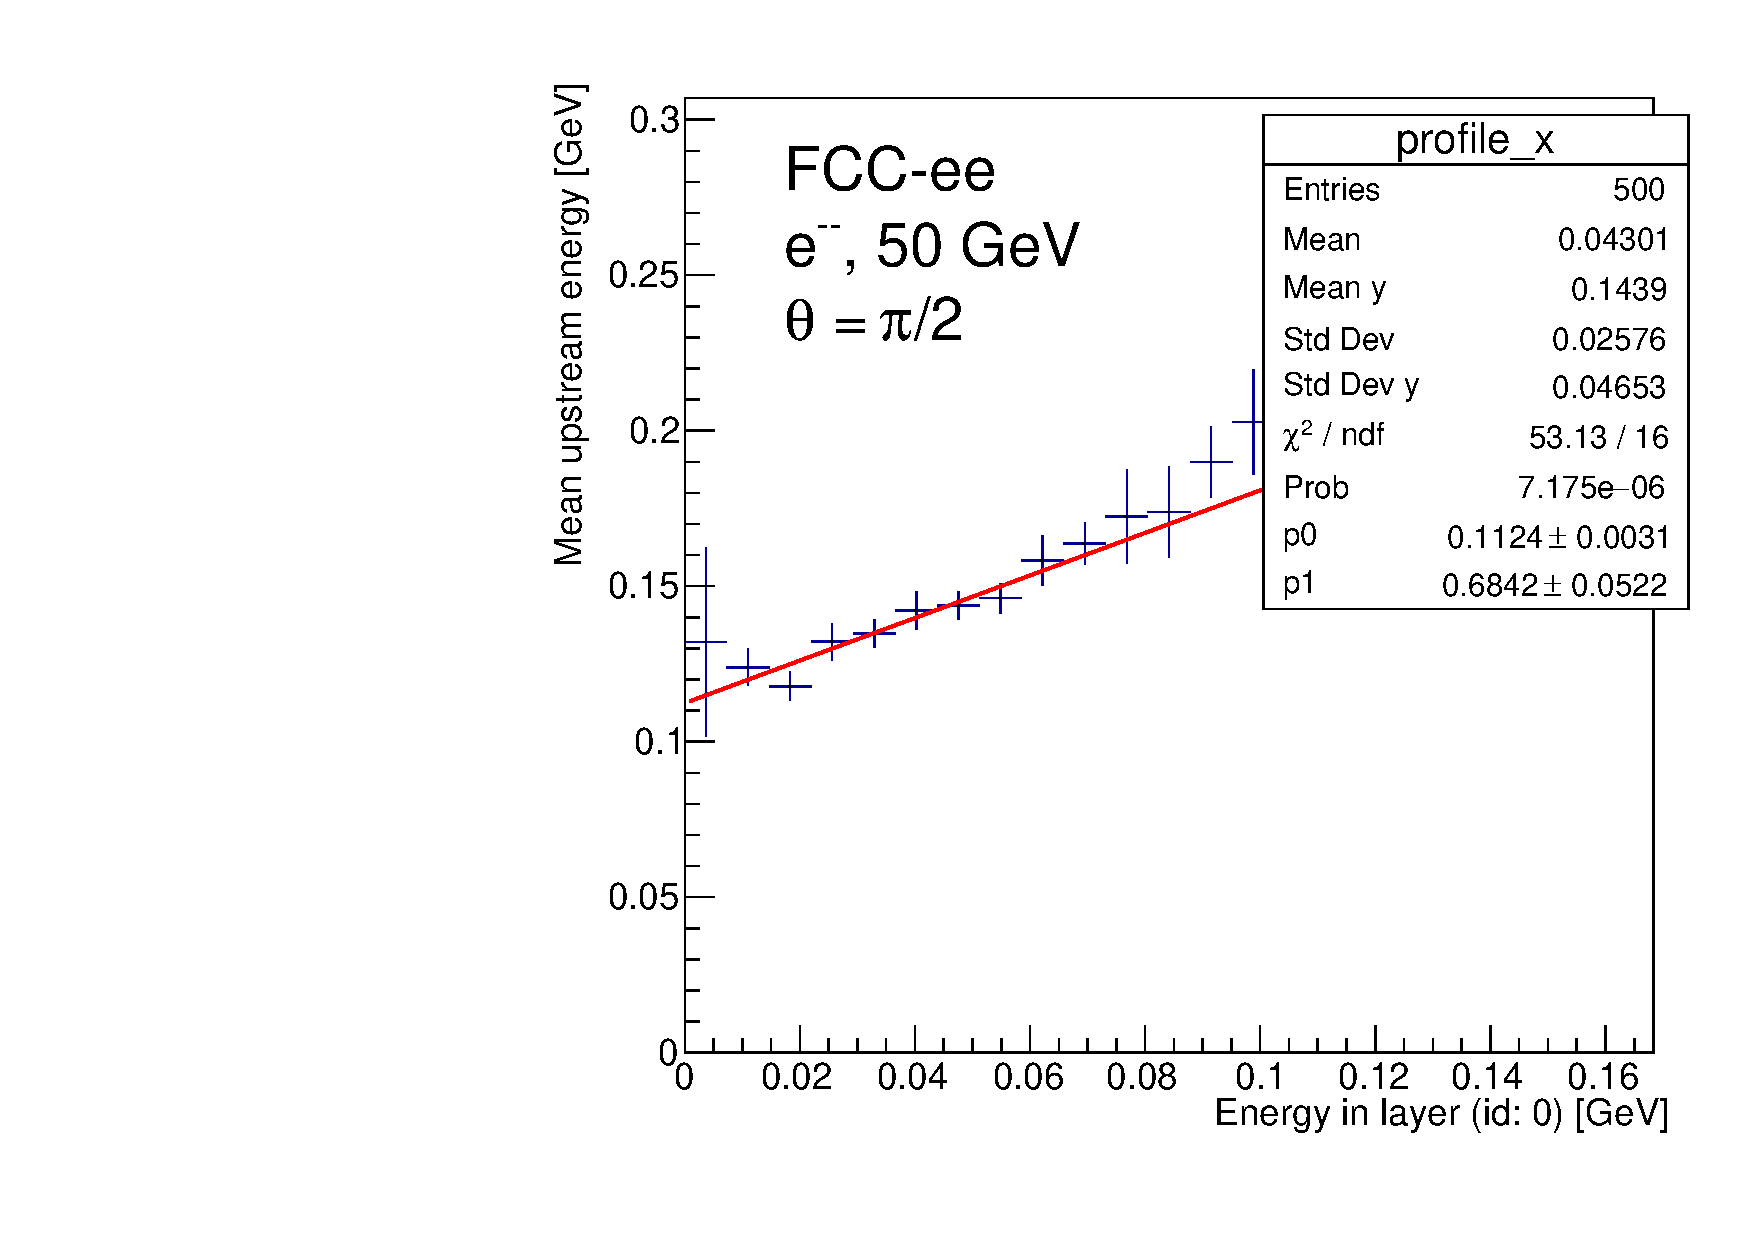
\includegraphics[width=0.49\linewidth]{figures/fccee_profile_upstream_vs_first_layer_90deg_50GeV.pdf}
\end{frame}

\begin{frame}
  \frametitle{FCC-ee: Energy in Layer vs. Cryo energy}

  \begin{itemize}
    \item No correlation between energy in full cryostat and energy in first
          layer
    \item Correlation between last layer (id: 7) and full cryostat energy
          \begin{itemize}
            \item Dominated by energy of the back cryostat
          \end{itemize}
    \item FCC-ee, $e^{-}$, 50 GeV, $\theta = \pi/2$
  \end{itemize}

  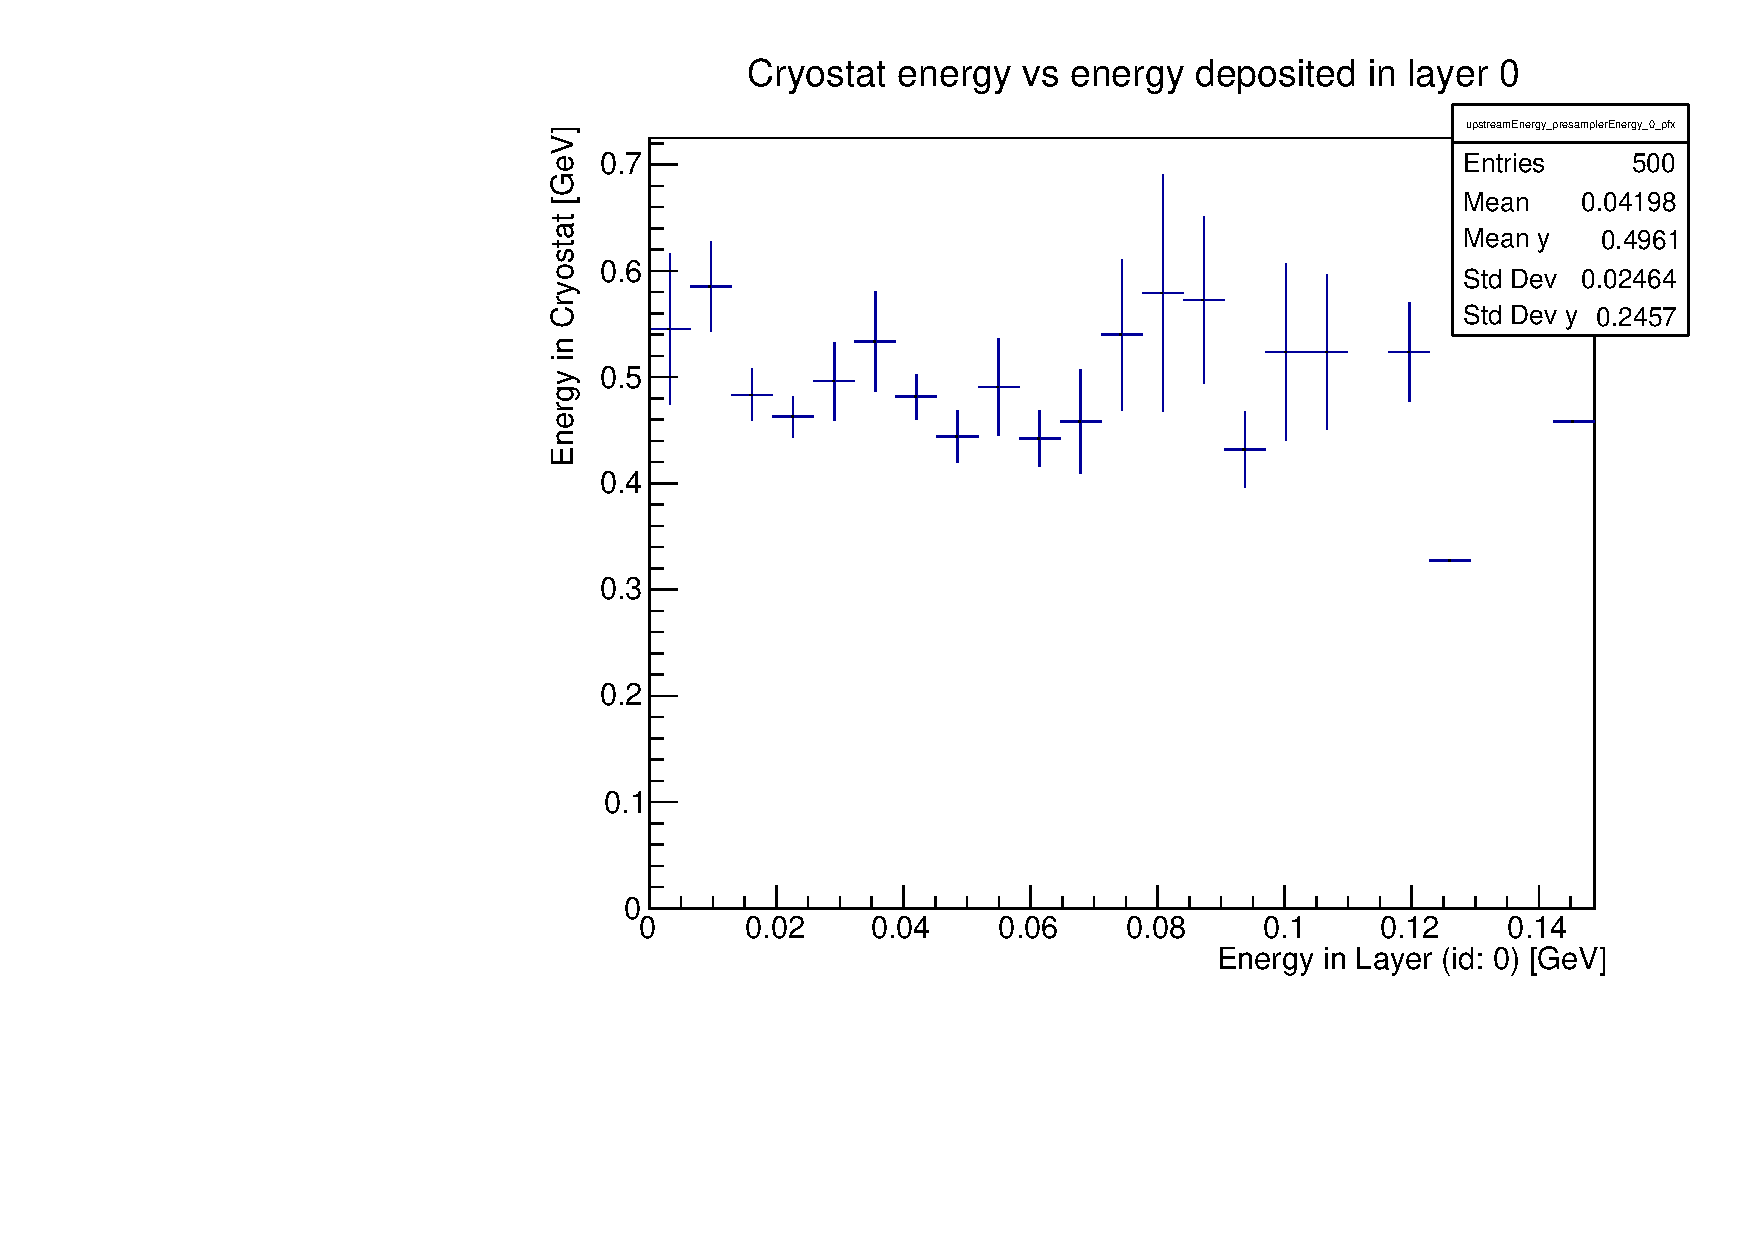
\includegraphics[width=0.49\linewidth]{figures/layer0_whole_cryo.pdf}
  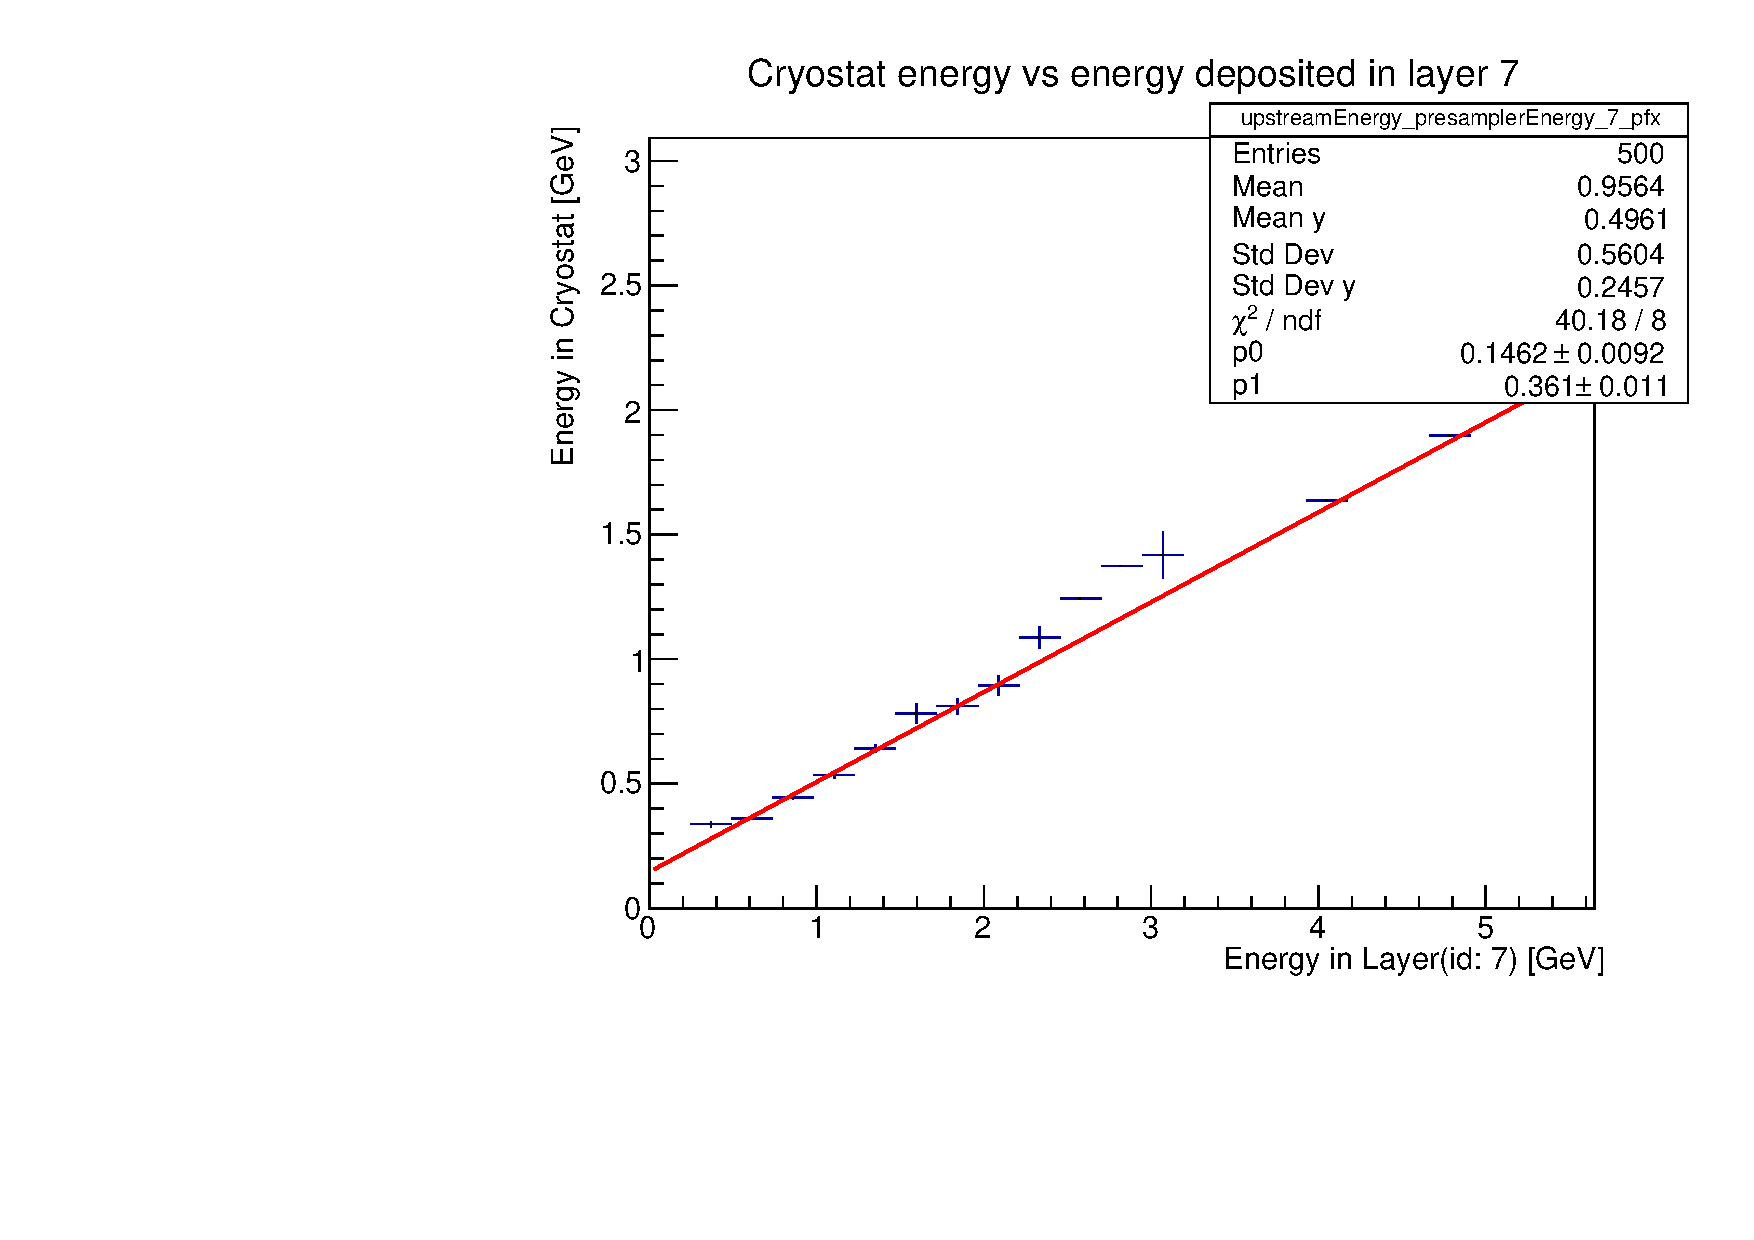
\includegraphics[width=0.49\linewidth]{figures/layer_7_whole_cryo.pdf}
\end{frame}


% ---------------------------------------------------------------------------- %
\section{Conclusions and Plans}

\begin{frame}
  \frametitle{Conclusion and Plans}

  \begin{itemize}
    \item For FCC-ee large energy leakage observed
    \item Also, upstream correction significantly smaller
    \item Further optimization to be discussed
    \item Replacement of upstream correction with other energy correction
    \item Investigate minor issues:
          \begin{itemize}
            \item No energy in back LAr bath
            \item Correlation between last layer and back cryostat
          \end{itemize}
  \end{itemize}
\end{frame}


\appendix
\backupbegin{}

\begin{frame}[c]
  \begin{center}
    \redtext{\Huge Backup}
  \end{center}
\end{frame}


\begin{frame}
  \frametitle{FCC-ee IDEA-LAr Upstream Correction}

  \redtext{FCC-ee} IDEA-LAr parametrization:

  \begin{equation*}
    E = E_\text{upstream} + E_\text{cluster}
  \end{equation*}

  \begin{equation*}
  E_\text{upstream} = P_0(E_\text{cluster}, |\eta|) +
                      P_1(E_\text{cluster}, |\eta|) \cdot E_\text{firstLayer}
  \end{equation*}

  \begin{equation*}
    P_0 = P_{00}(|\eta|) + P_{01}(|\eta|) \cdot E_{cluster}  \qquad
    P_1 = \bluetext{?}
  \end{equation*}

  \begin{center}
    $\eta$ dependence \bluetext{?}
  \end{center}
\end{frame}


% ---------------------------------------------------------------------------- %
\section{Momentum dependence}
\begin{frame}
  \frametitle{FCC-ee IDEA-LAr Upstream Correction}

  \begin{center}
    Energy dependence, Layer \redtext{ID:\@ 0} \\
    $P_1 = P_{10}(|\eta|) + P_{11}(|\eta|) \cdot E_{cluster}$
  \end{center}

  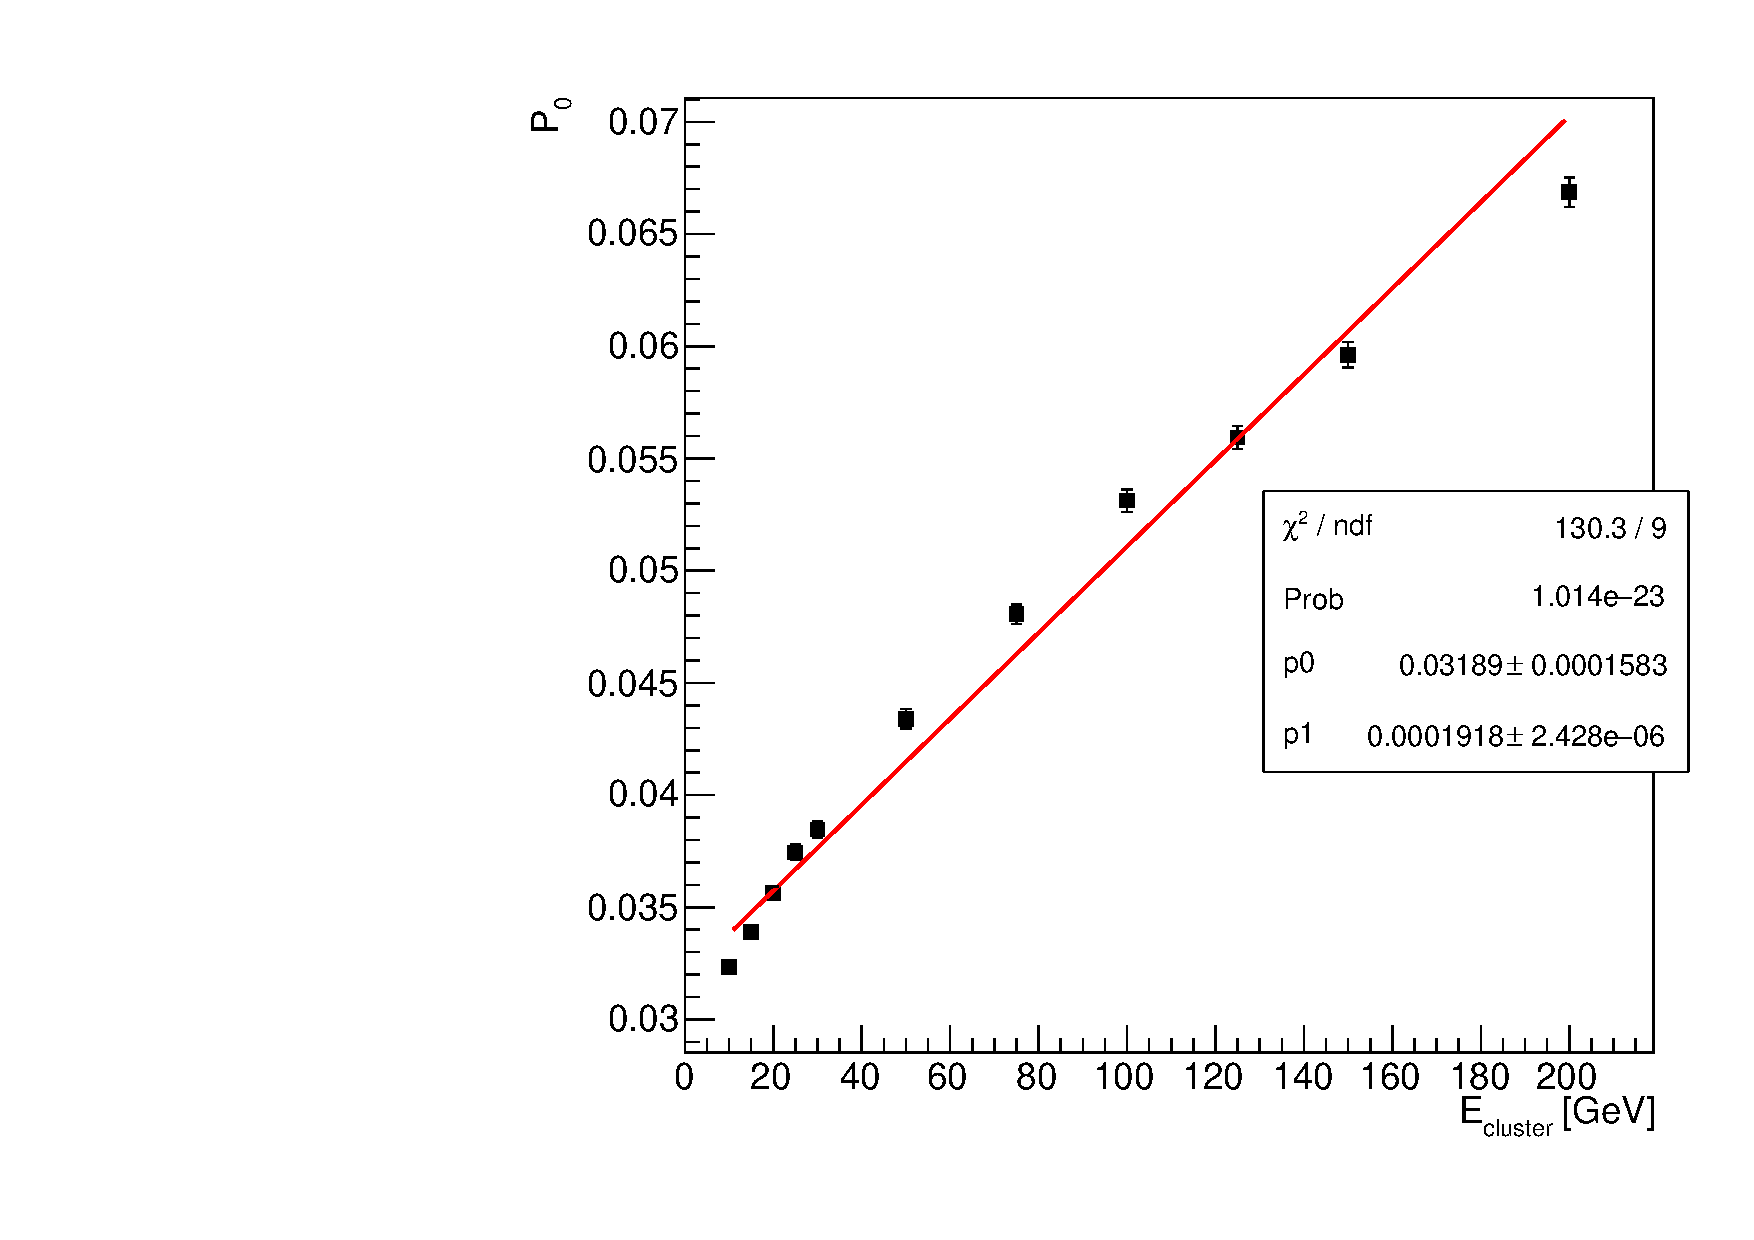
\includegraphics[width=0.49\linewidth]{figures/momentum_id0/graph_upstream_corr_param0.pdf}
  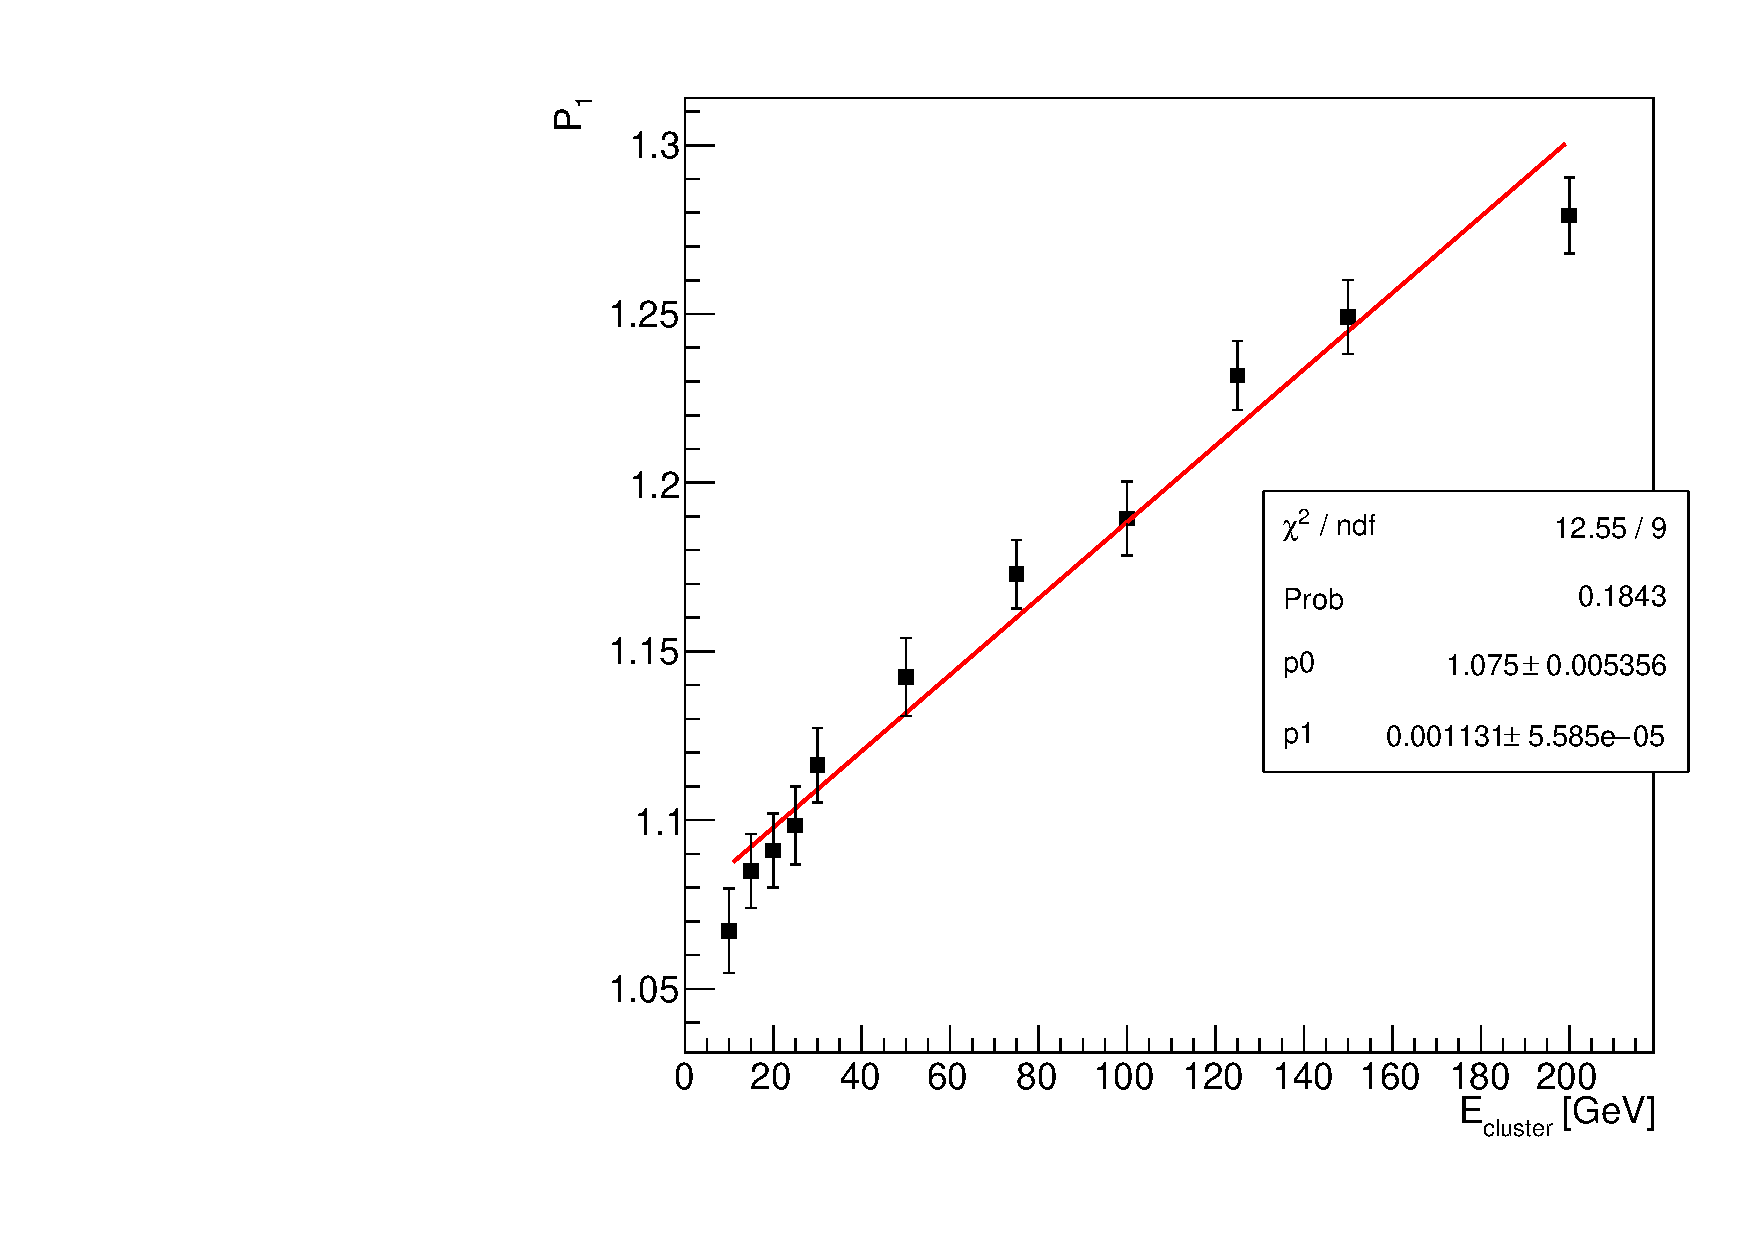
\includegraphics[width=0.49\linewidth]{figures/momentum_id0/graph_upstream_corr_param1.pdf}
\end{frame}

\begin{frame}
  \frametitle{FCC-ee IDEA-LAr Upstream Correction}

  \begin{center}
    Energy dependence, Layer \redtext{ID:\@ 1} \\
    $ P_1 = P_{10}(|\eta|) + \frac{P_{11}(|\eta|)}{\sqrt{E_{cluster}}} $
  \end{center}

  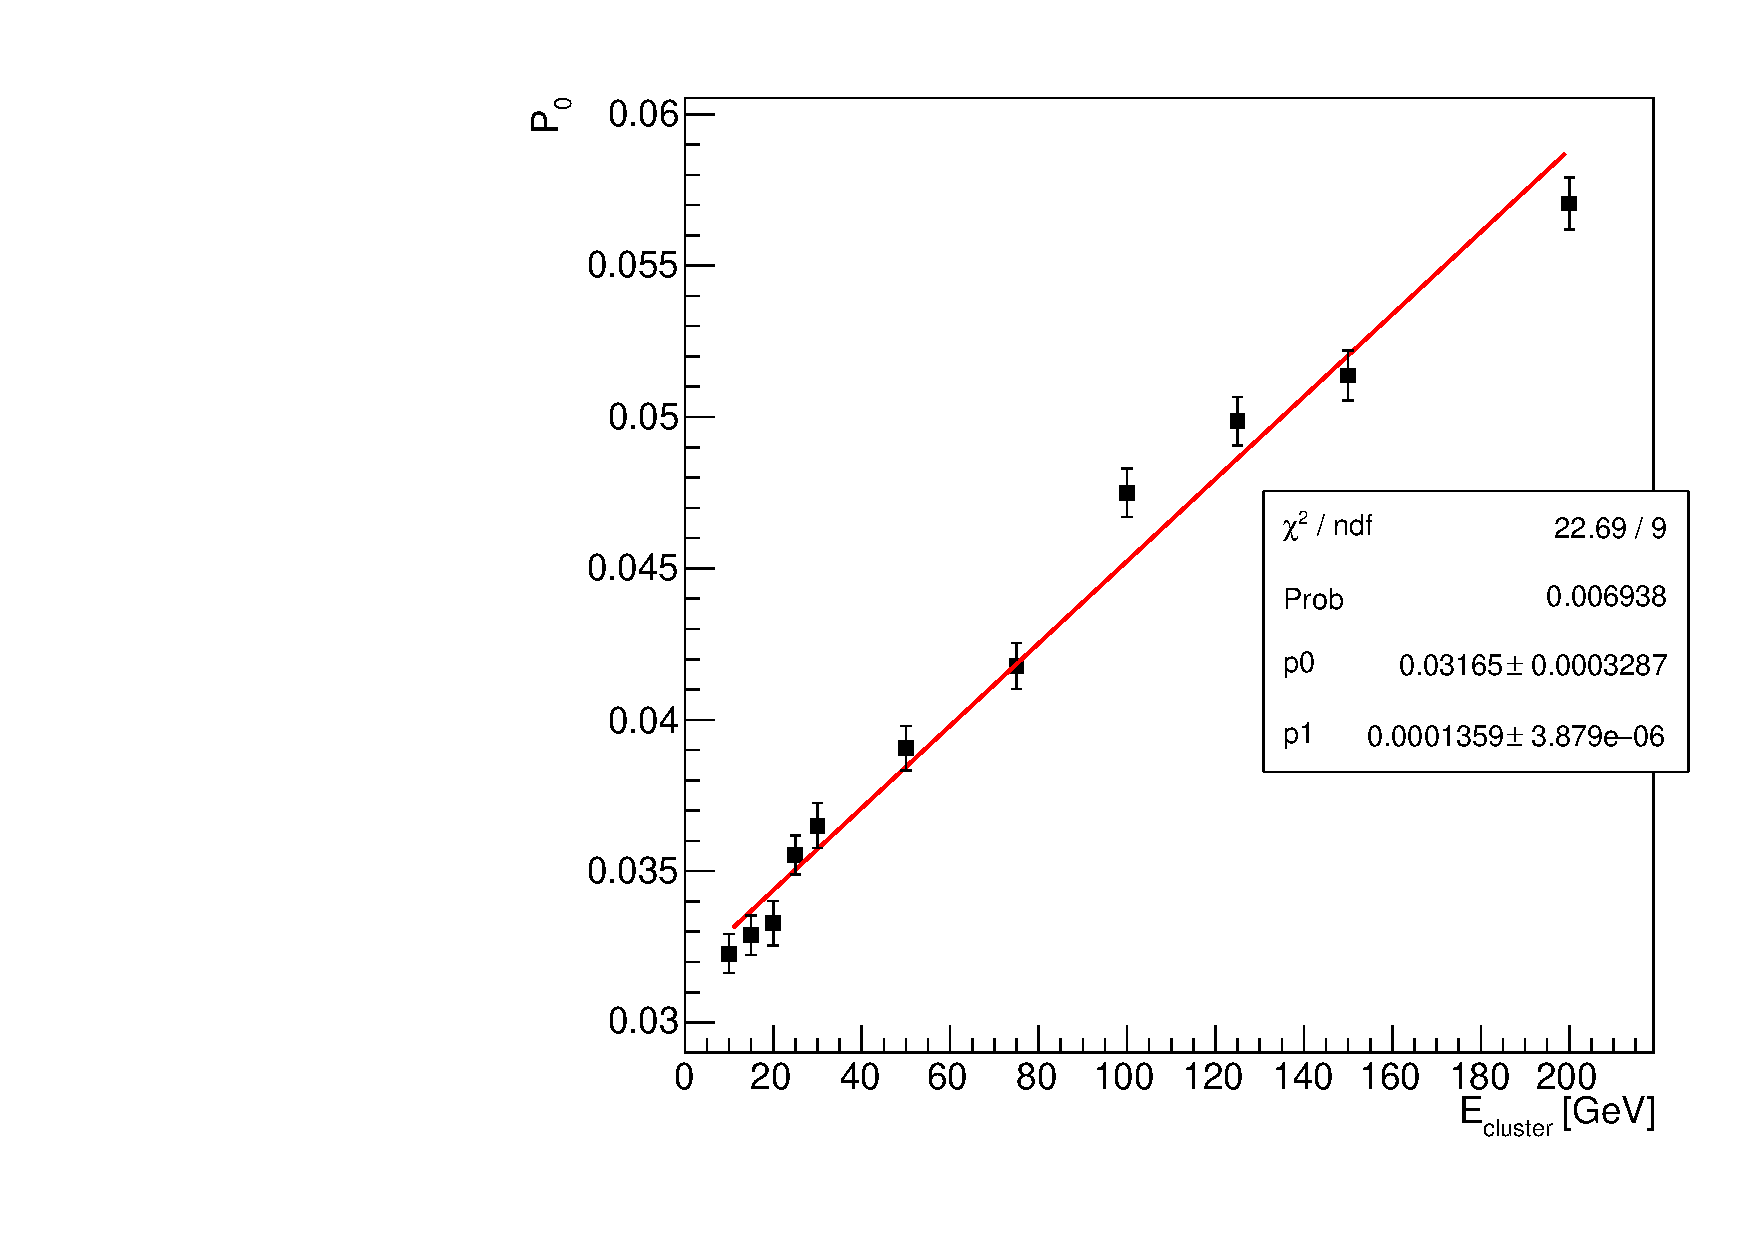
\includegraphics[width=0.49\linewidth]{figures/momentum_id1/graph_upstream_corr_param0.pdf}
  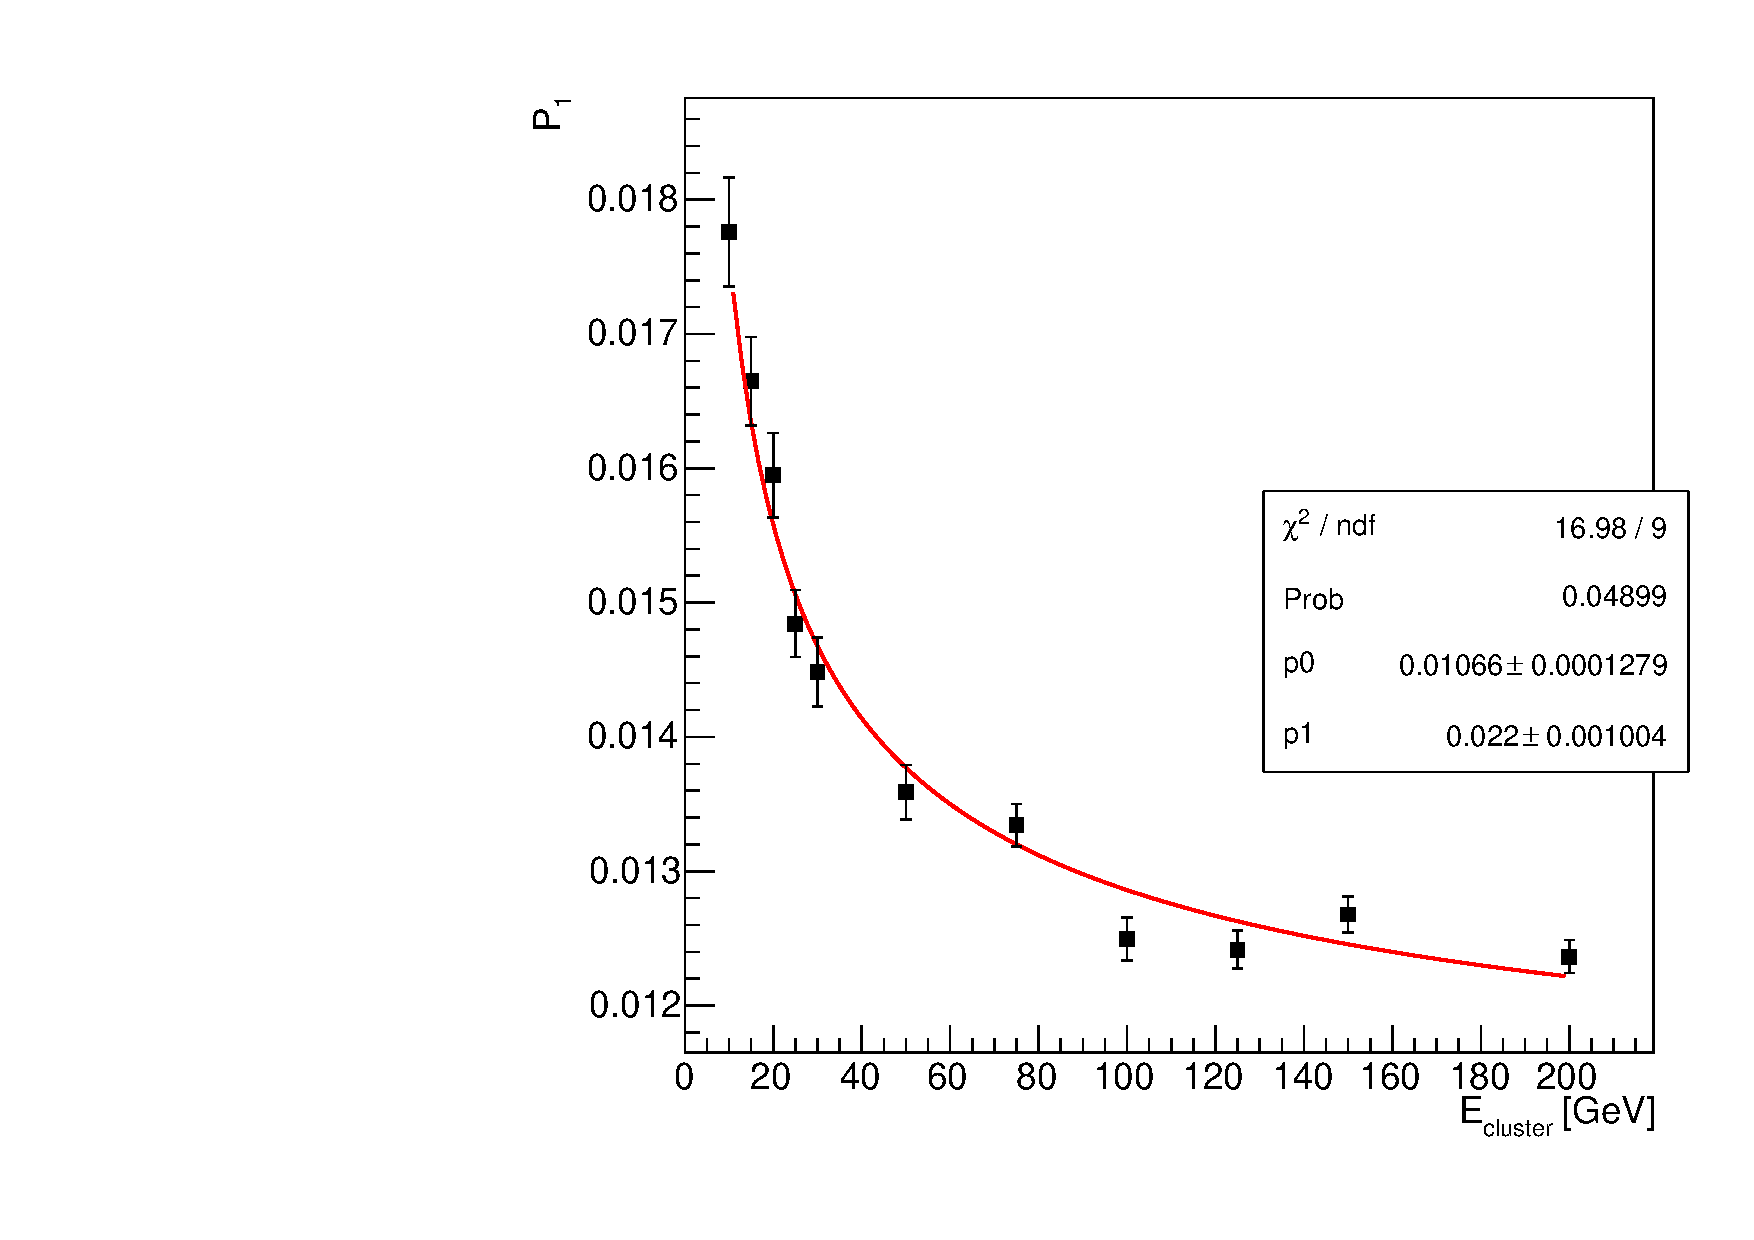
\includegraphics[width=0.49\linewidth]{figures/momentum_id1/graph_upstream_corr_param1.pdf}
\end{frame}

\begin{frame}
  \frametitle{At 10 GeV}

  \centering
  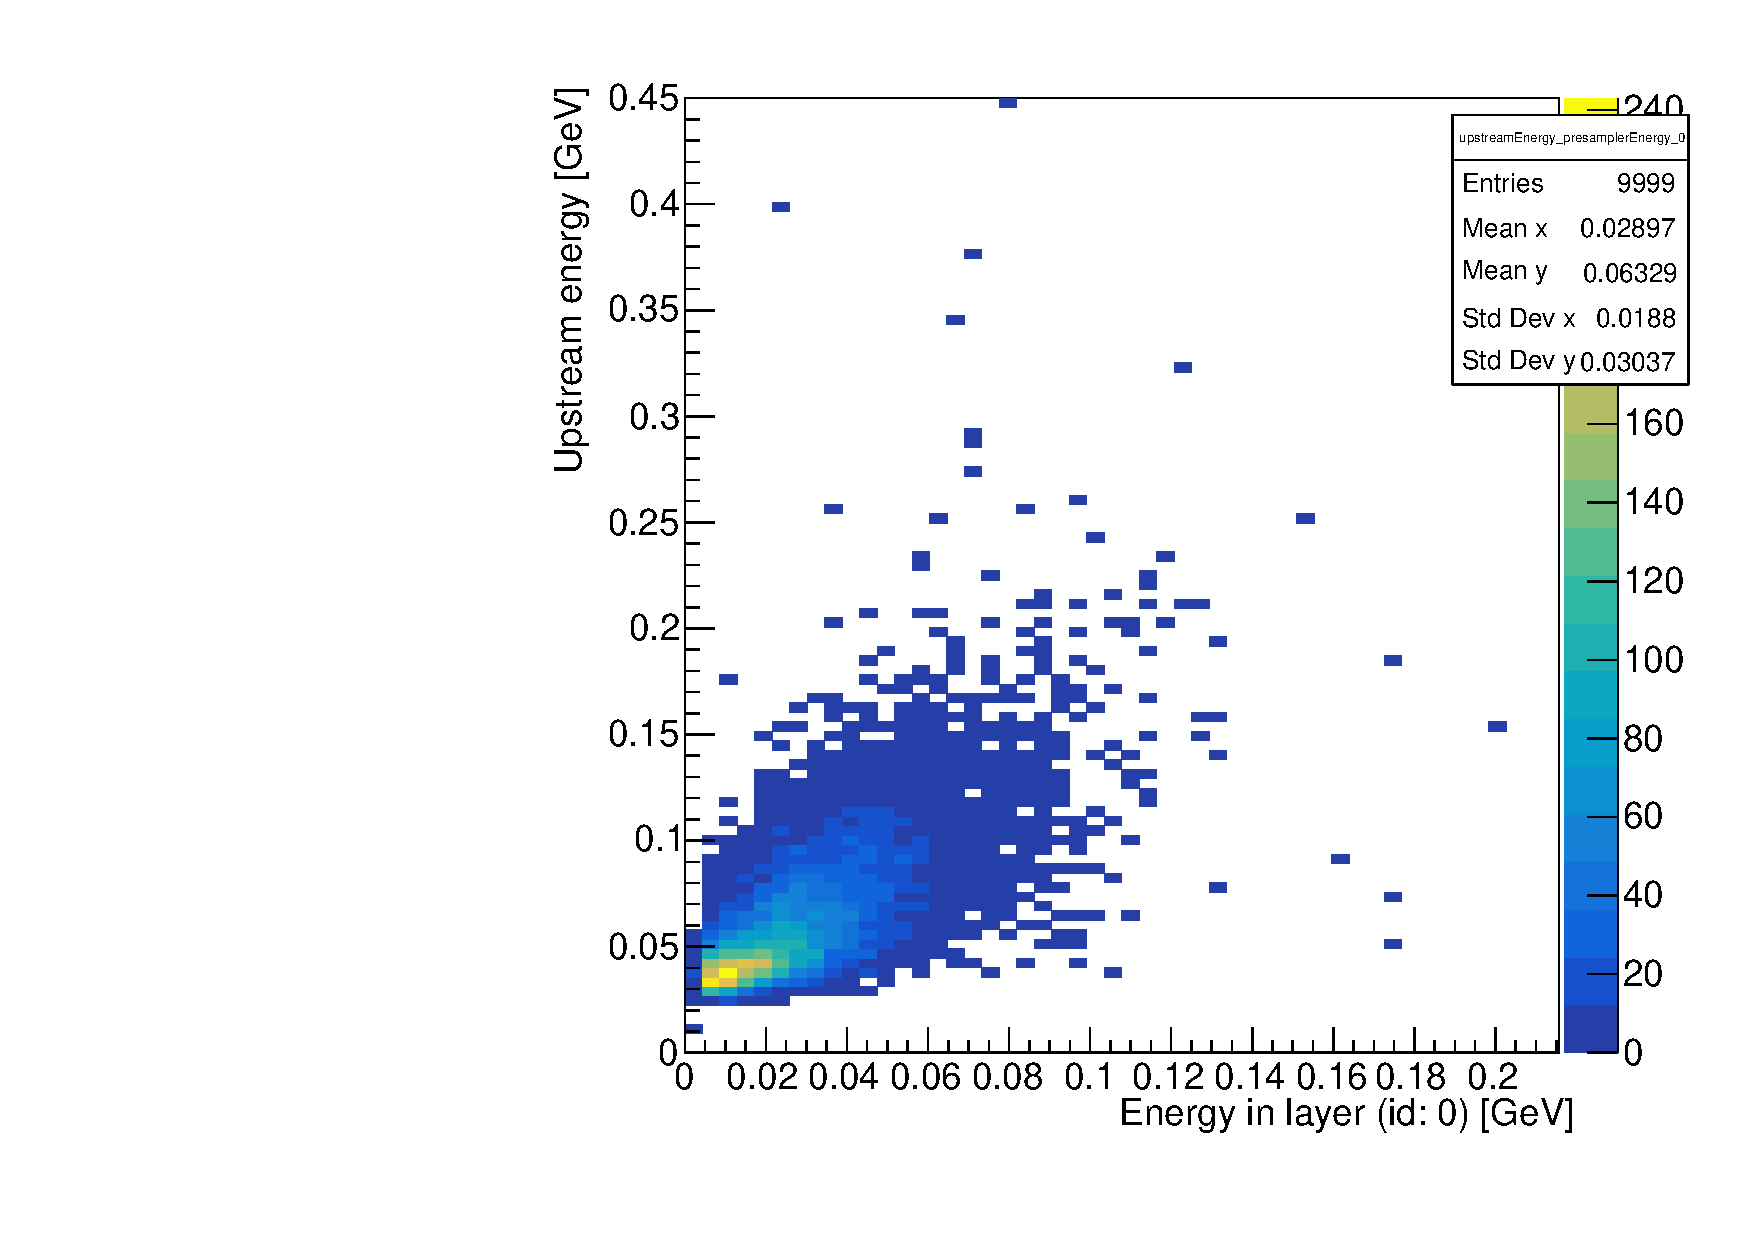
\includegraphics[width=0.39\linewidth]{figures/momentum_id0/hist_upstream_vs_first_layer_90deg_10GeV.pdf}
  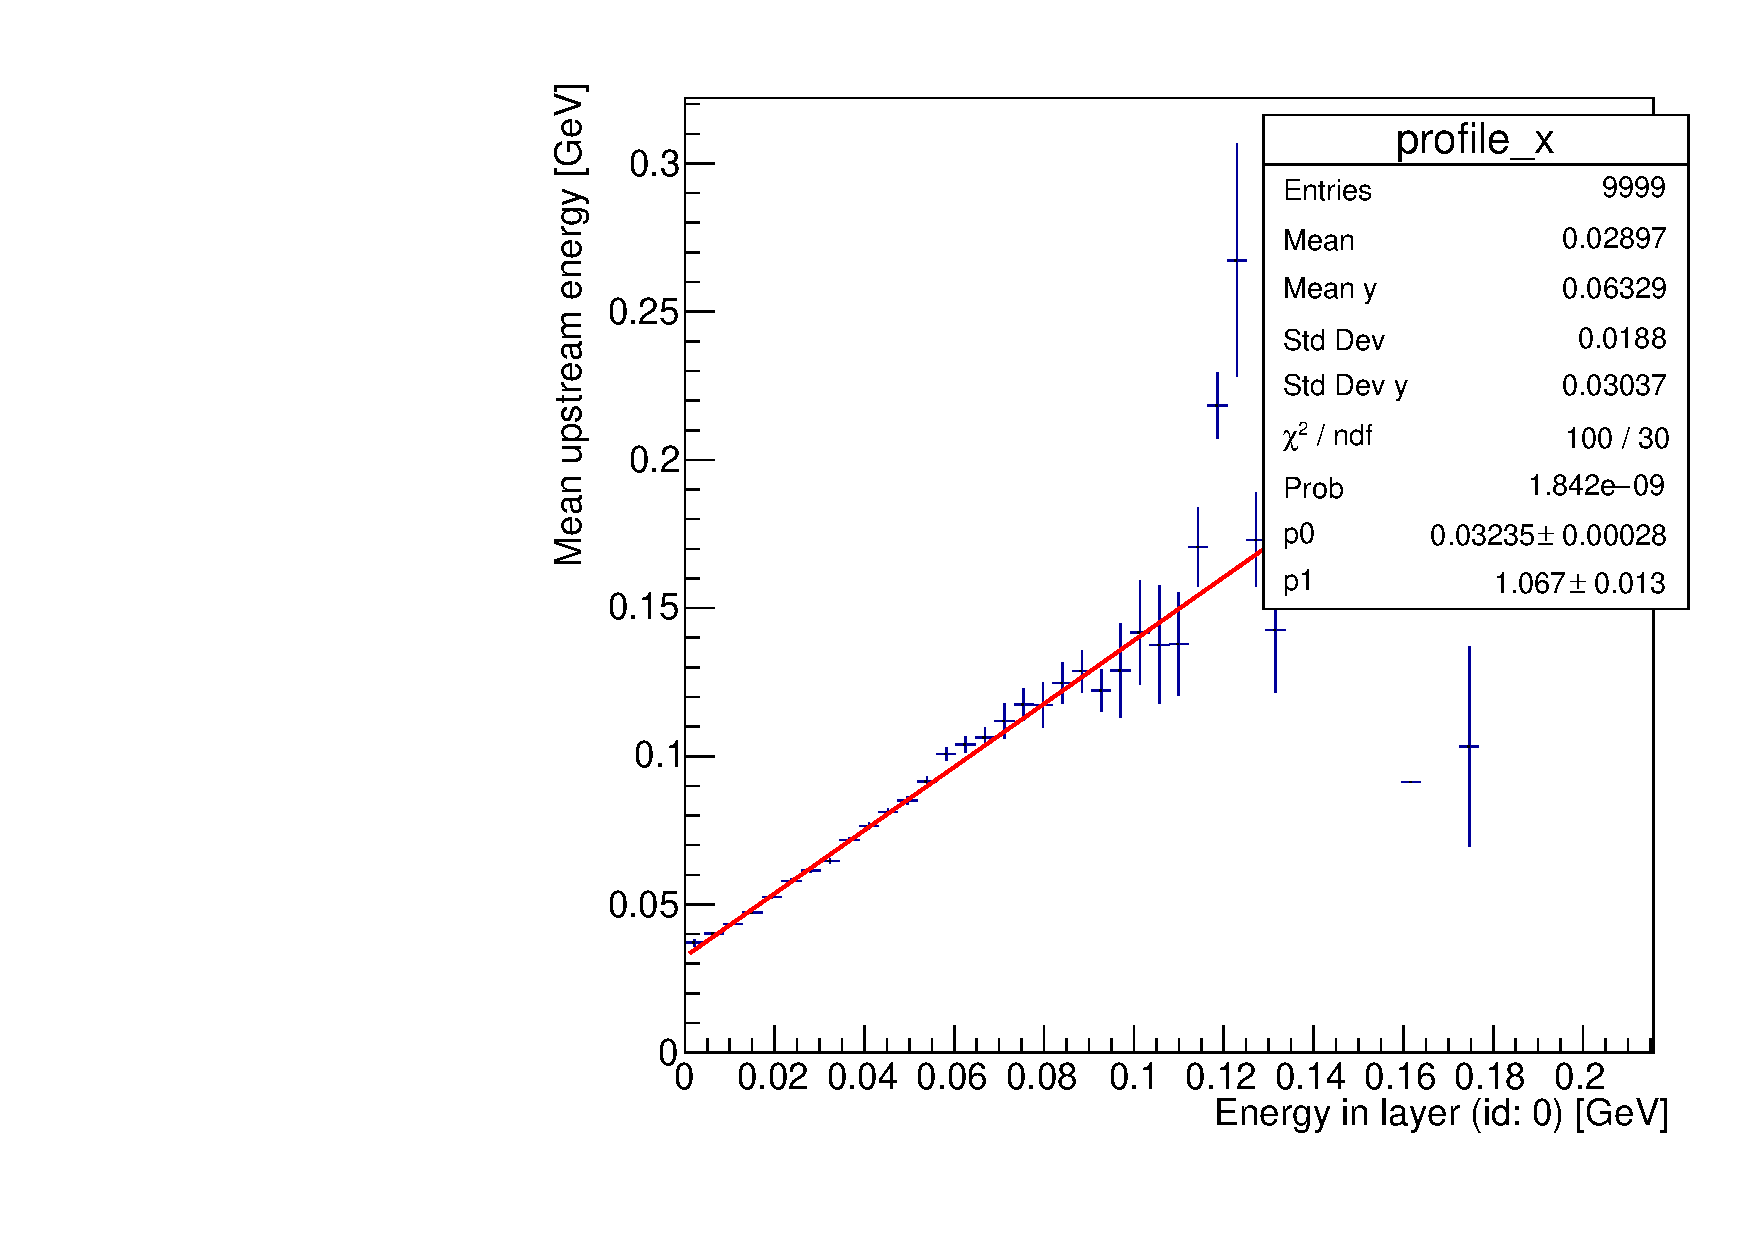
\includegraphics[width=0.39\linewidth]{figures/momentum_id0/profile_upstream_vs_first_layer_90deg_10GeV.pdf} \\
  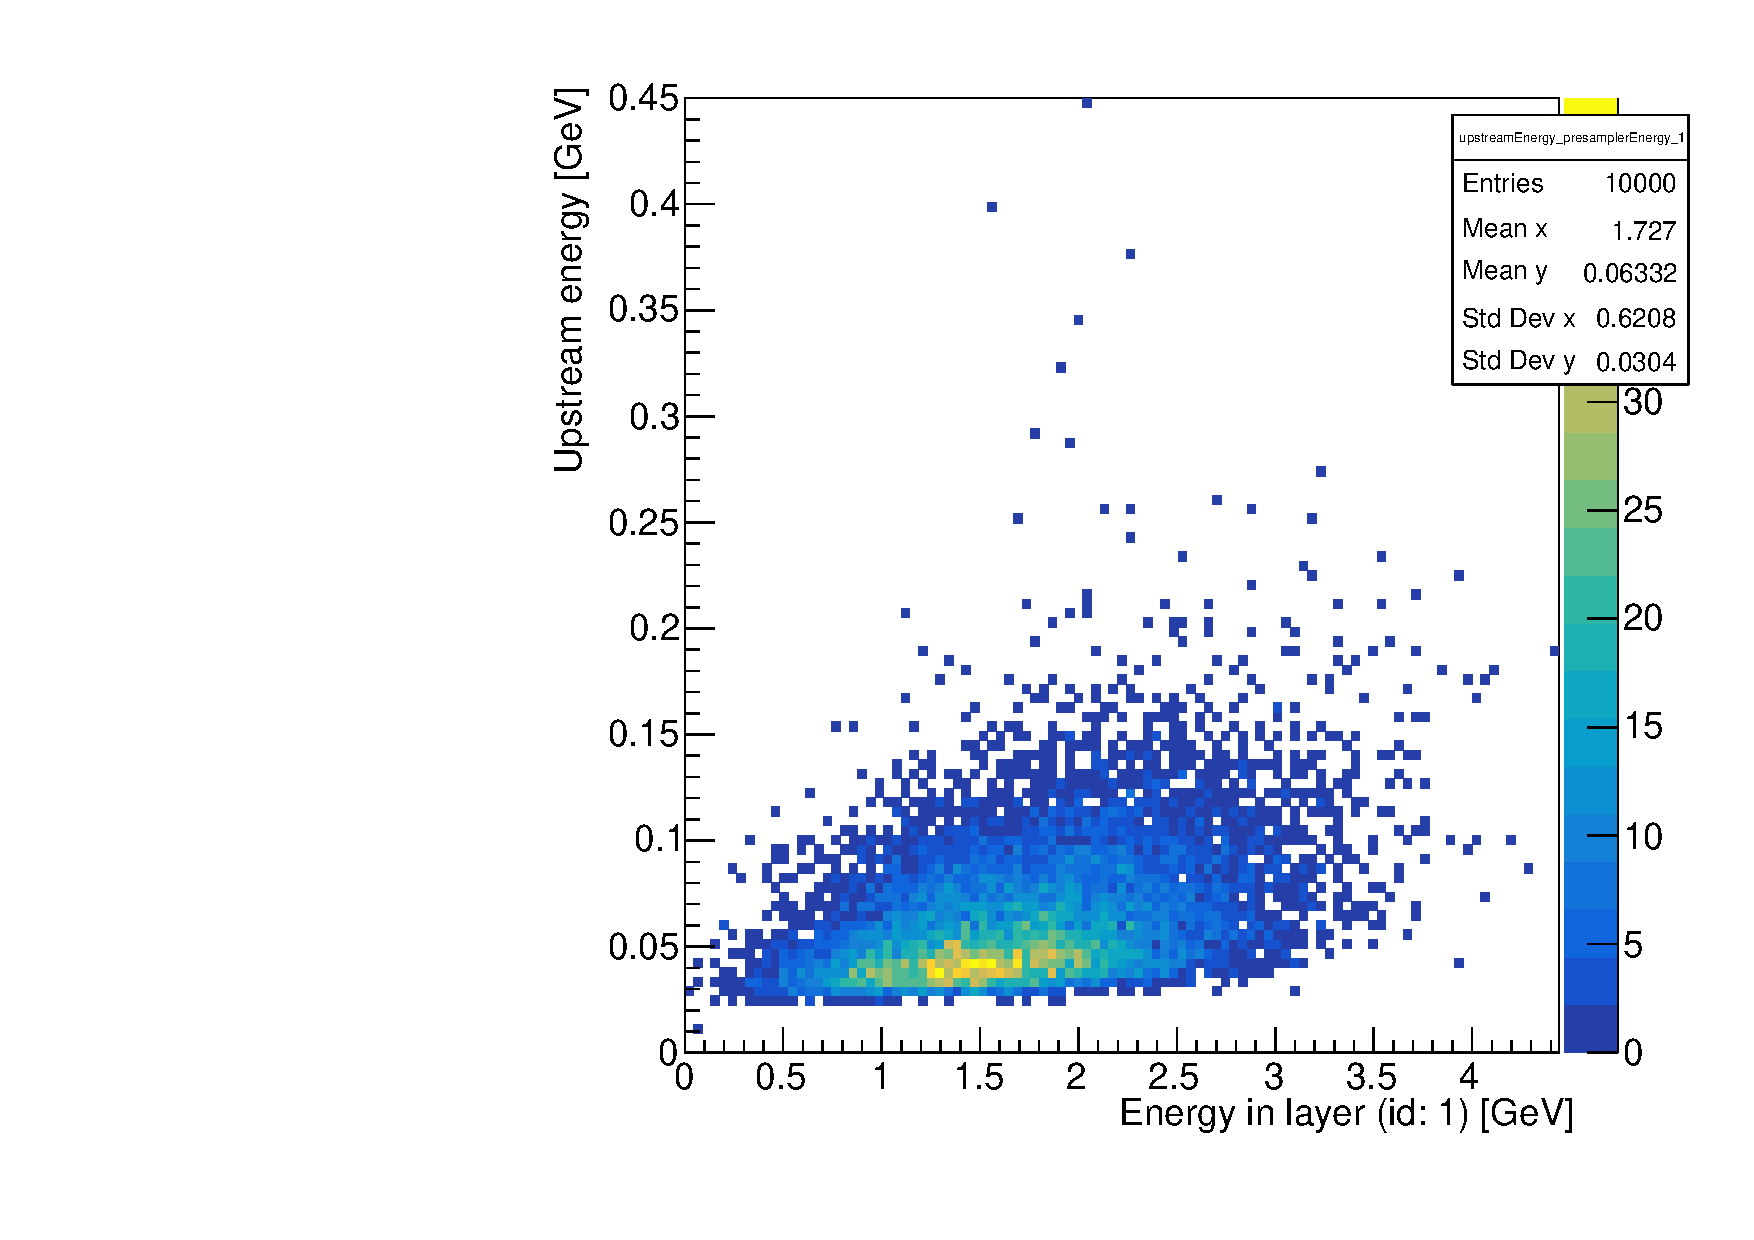
\includegraphics[width=0.39\linewidth]{figures/momentum_id1/hist_upstream_vs_first_layer_90deg_10GeV.pdf}
  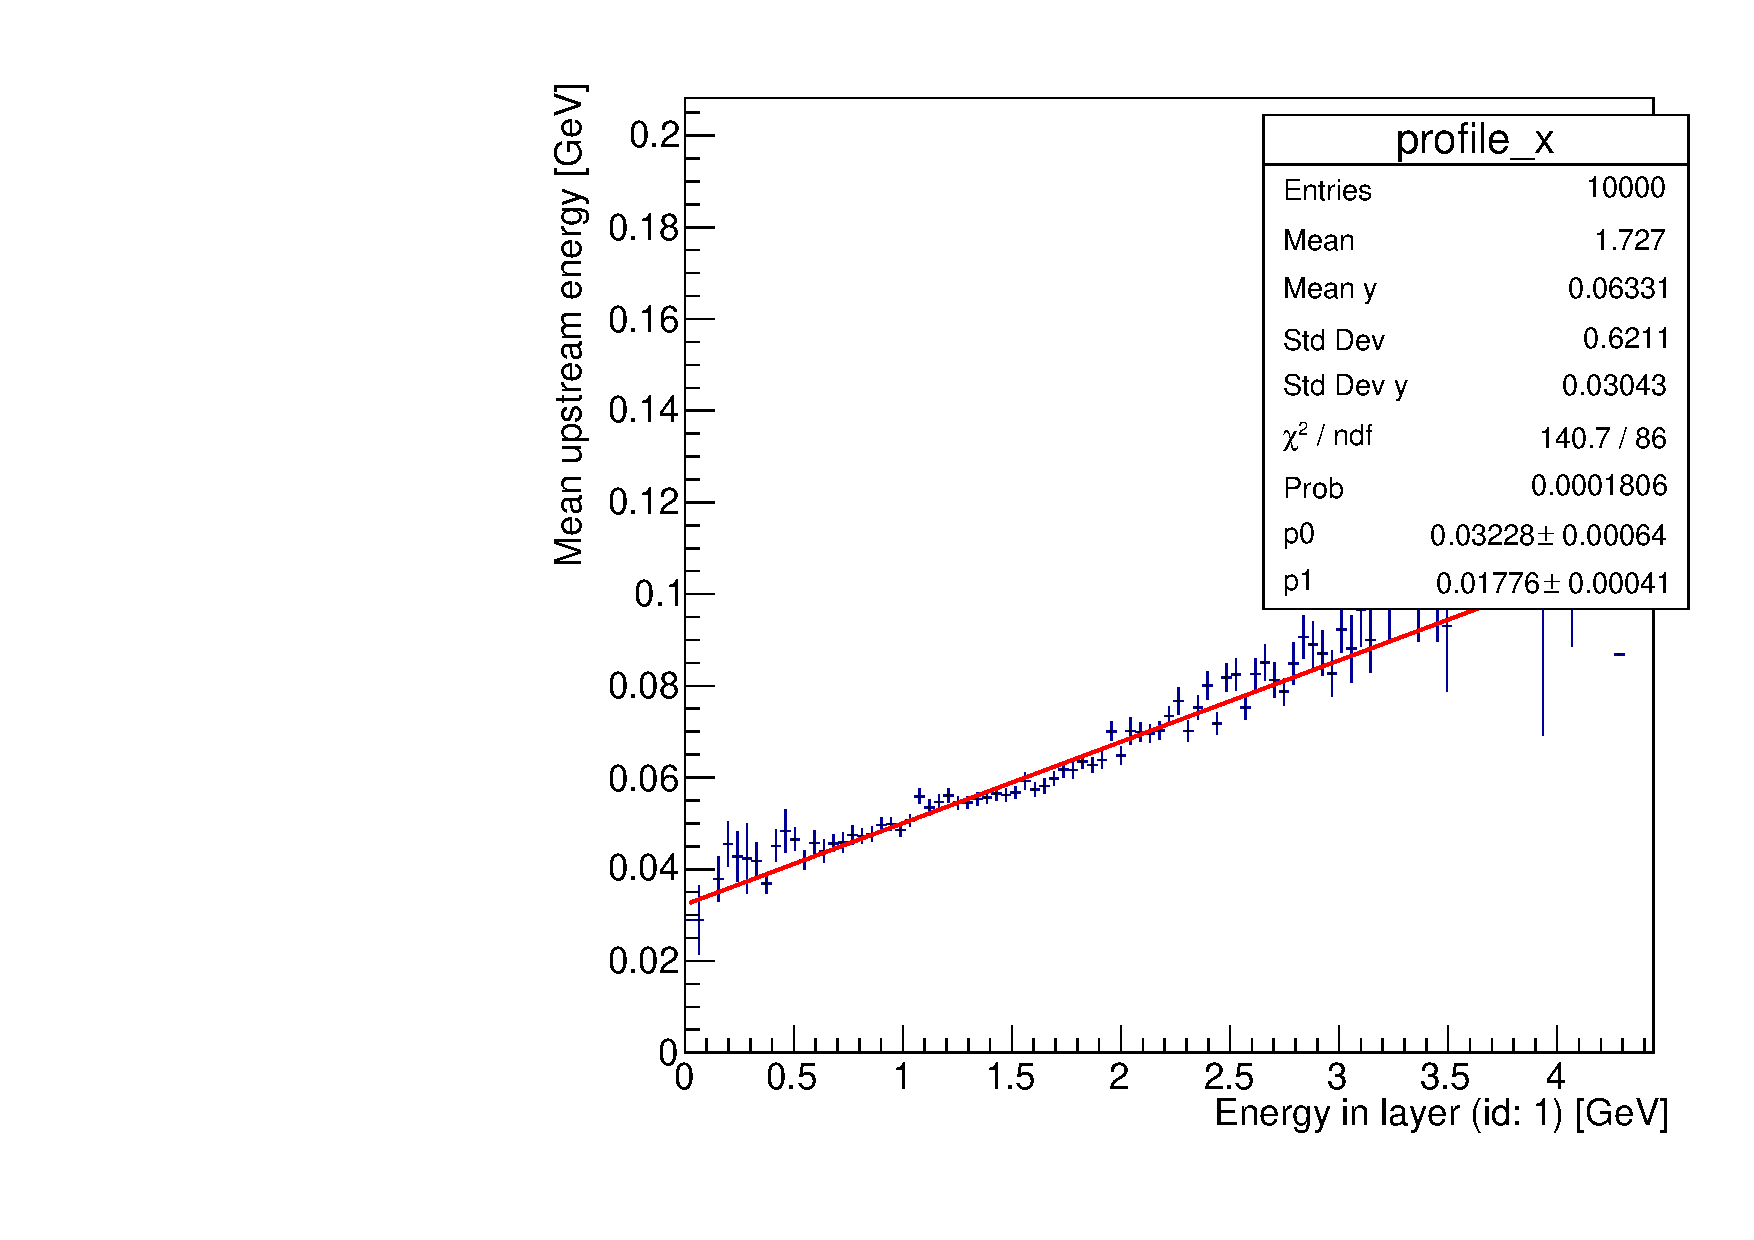
\includegraphics[width=0.39\linewidth]{figures/momentum_id1/profile_upstream_vs_first_layer_90deg_10GeV.pdf}
\end{frame}

\begin{frame}
  \frametitle{At 15 GeV}

  \centering
  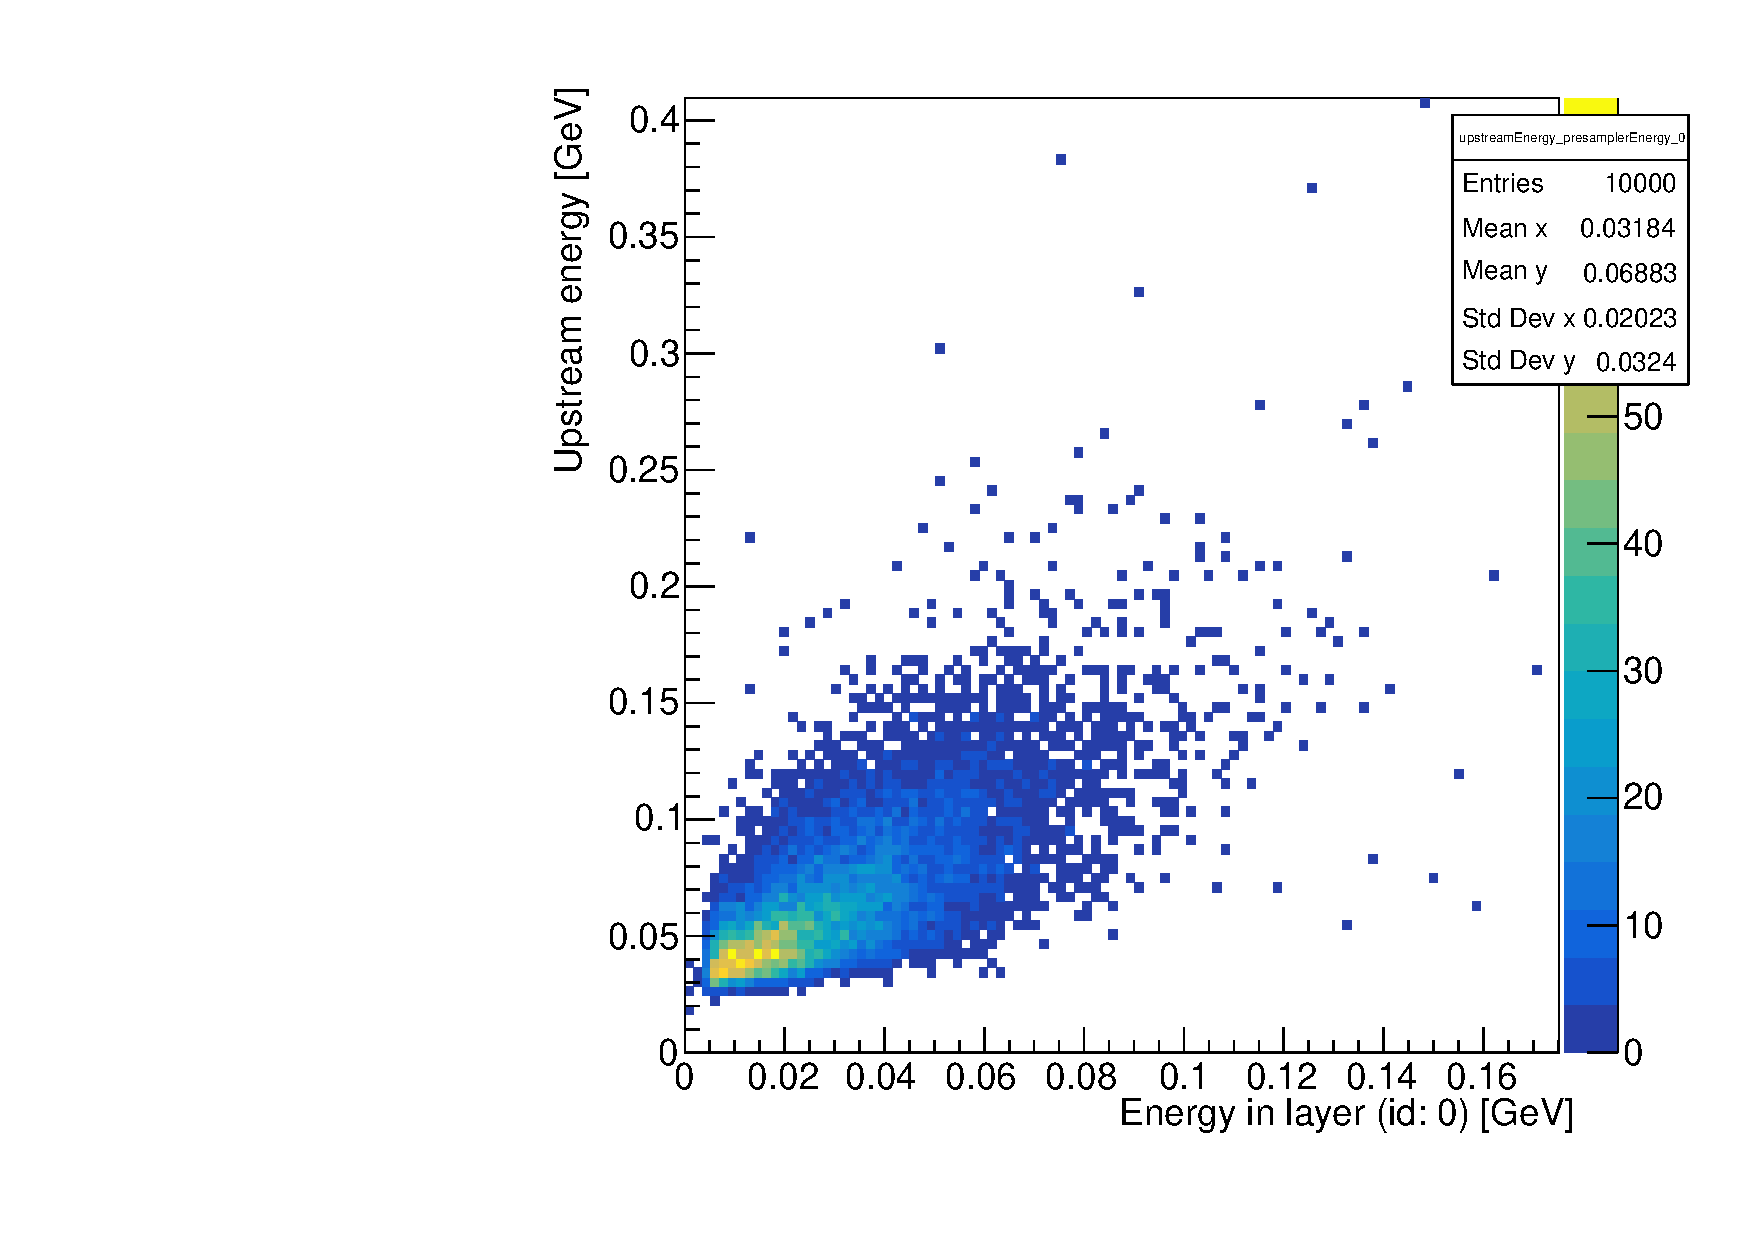
\includegraphics[width=0.39\linewidth]{figures/momentum_id0/hist_upstream_vs_first_layer_90deg_15GeV.pdf}
  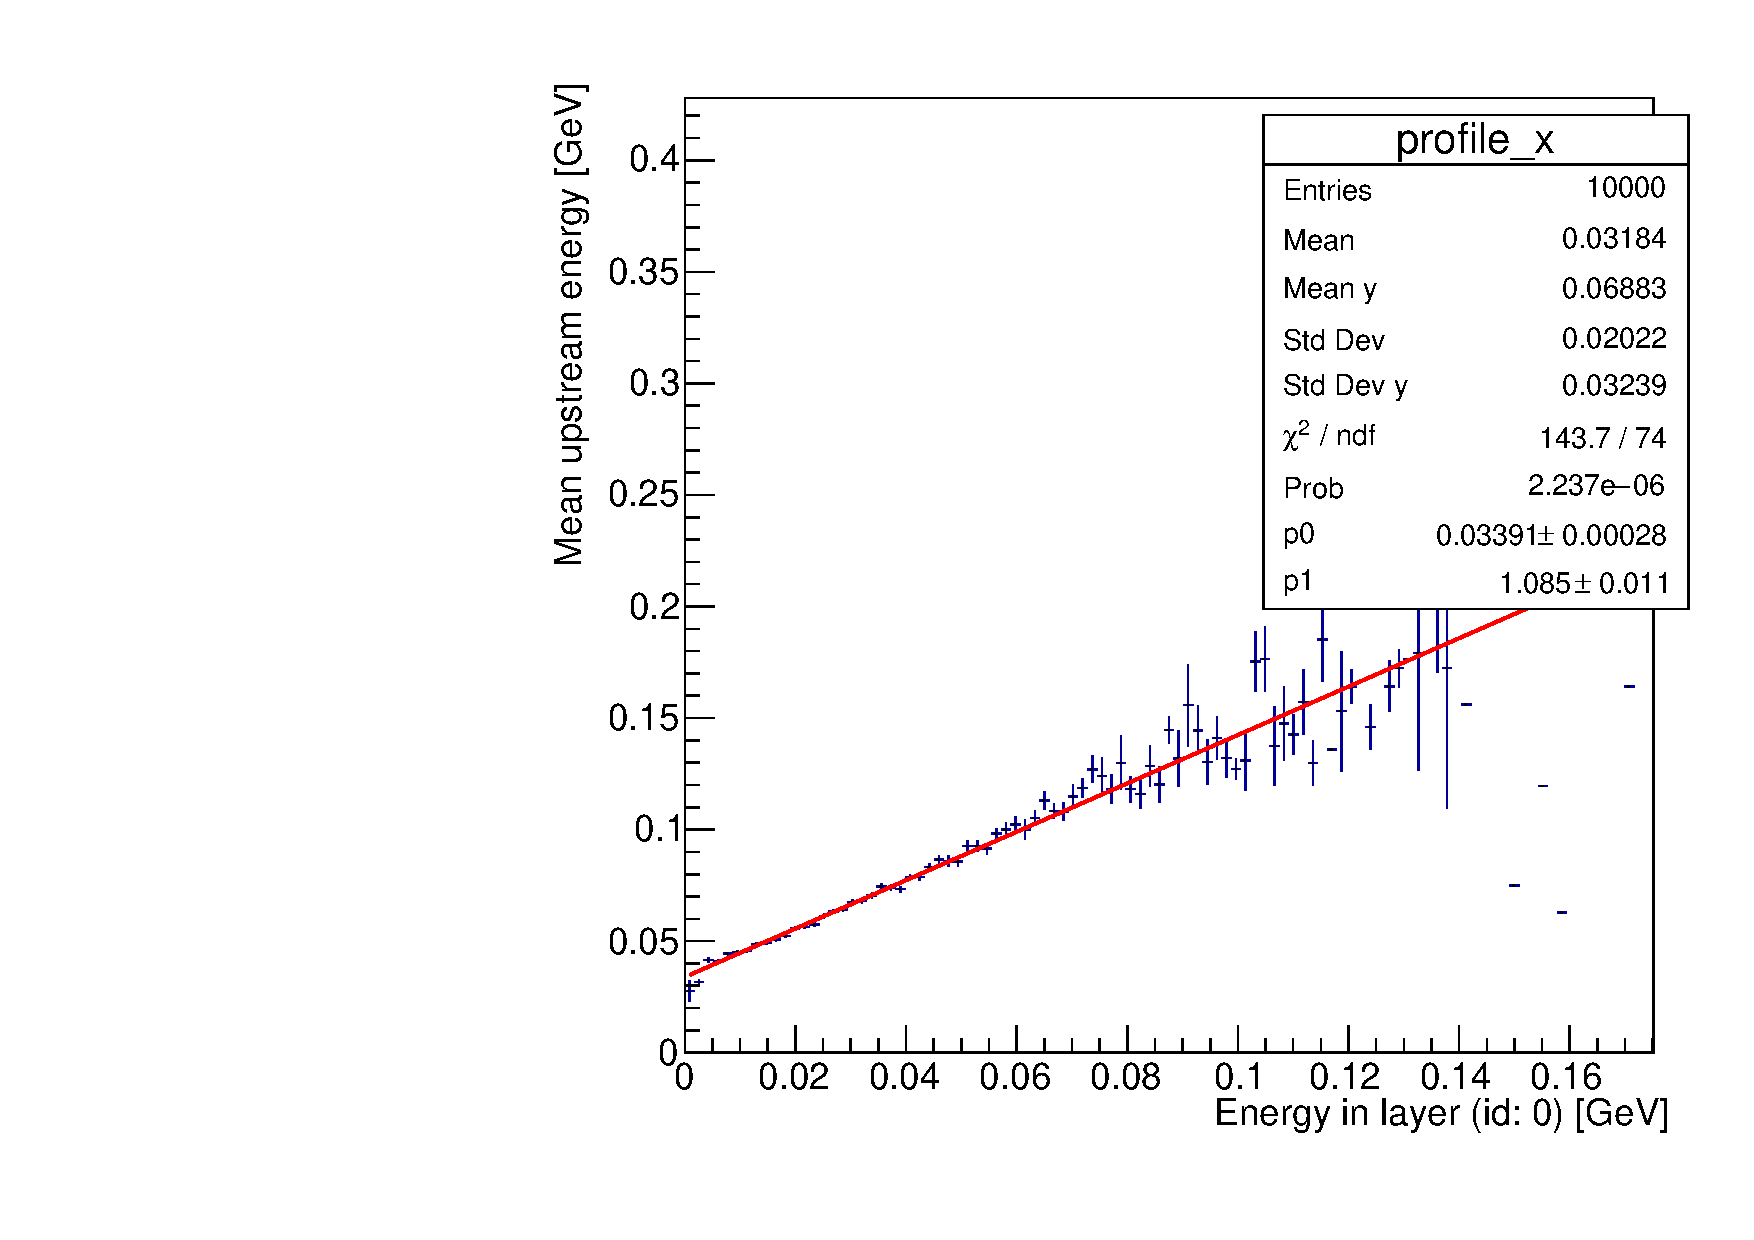
\includegraphics[width=0.39\linewidth]{figures/momentum_id0/profile_upstream_vs_first_layer_90deg_15GeV.pdf} \\
  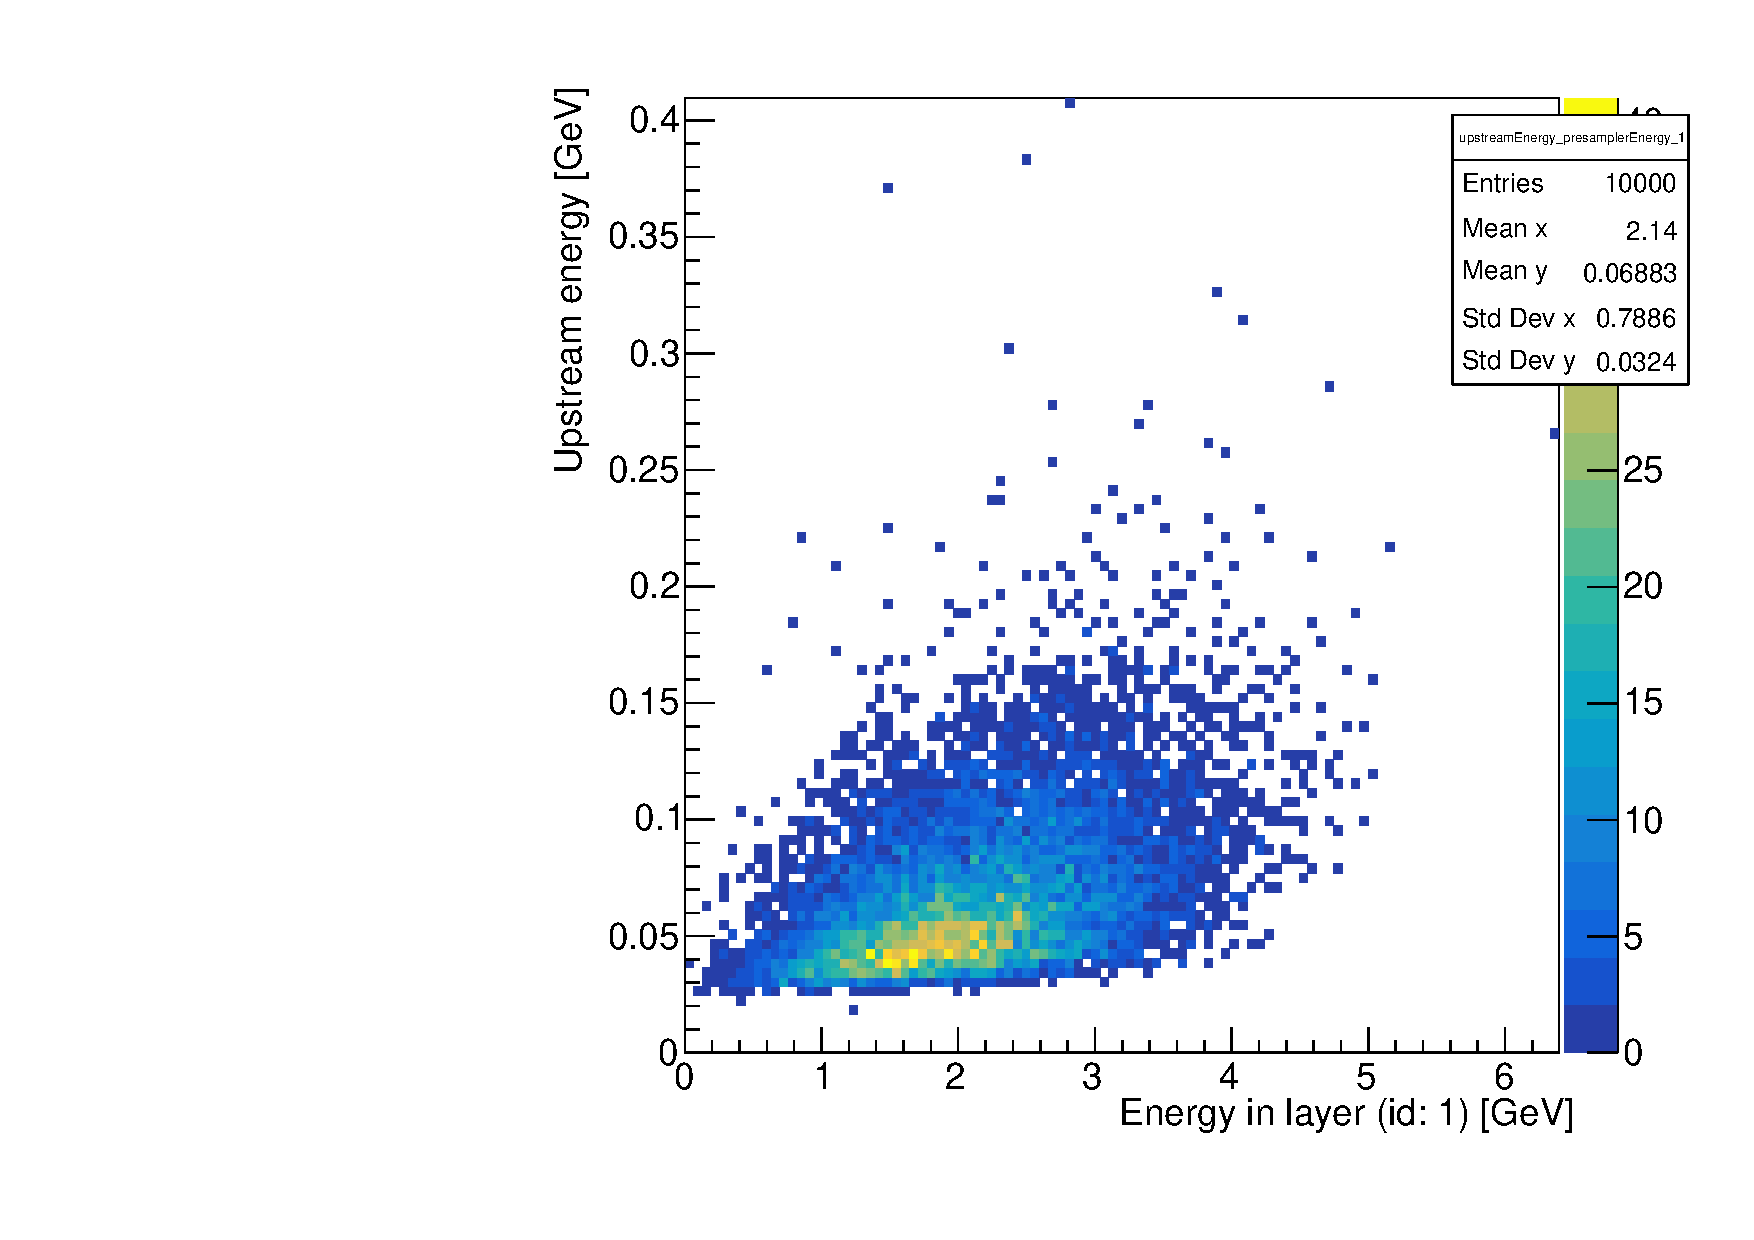
\includegraphics[width=0.39\linewidth]{figures/momentum_id1/hist_upstream_vs_first_layer_90deg_15GeV.pdf}
  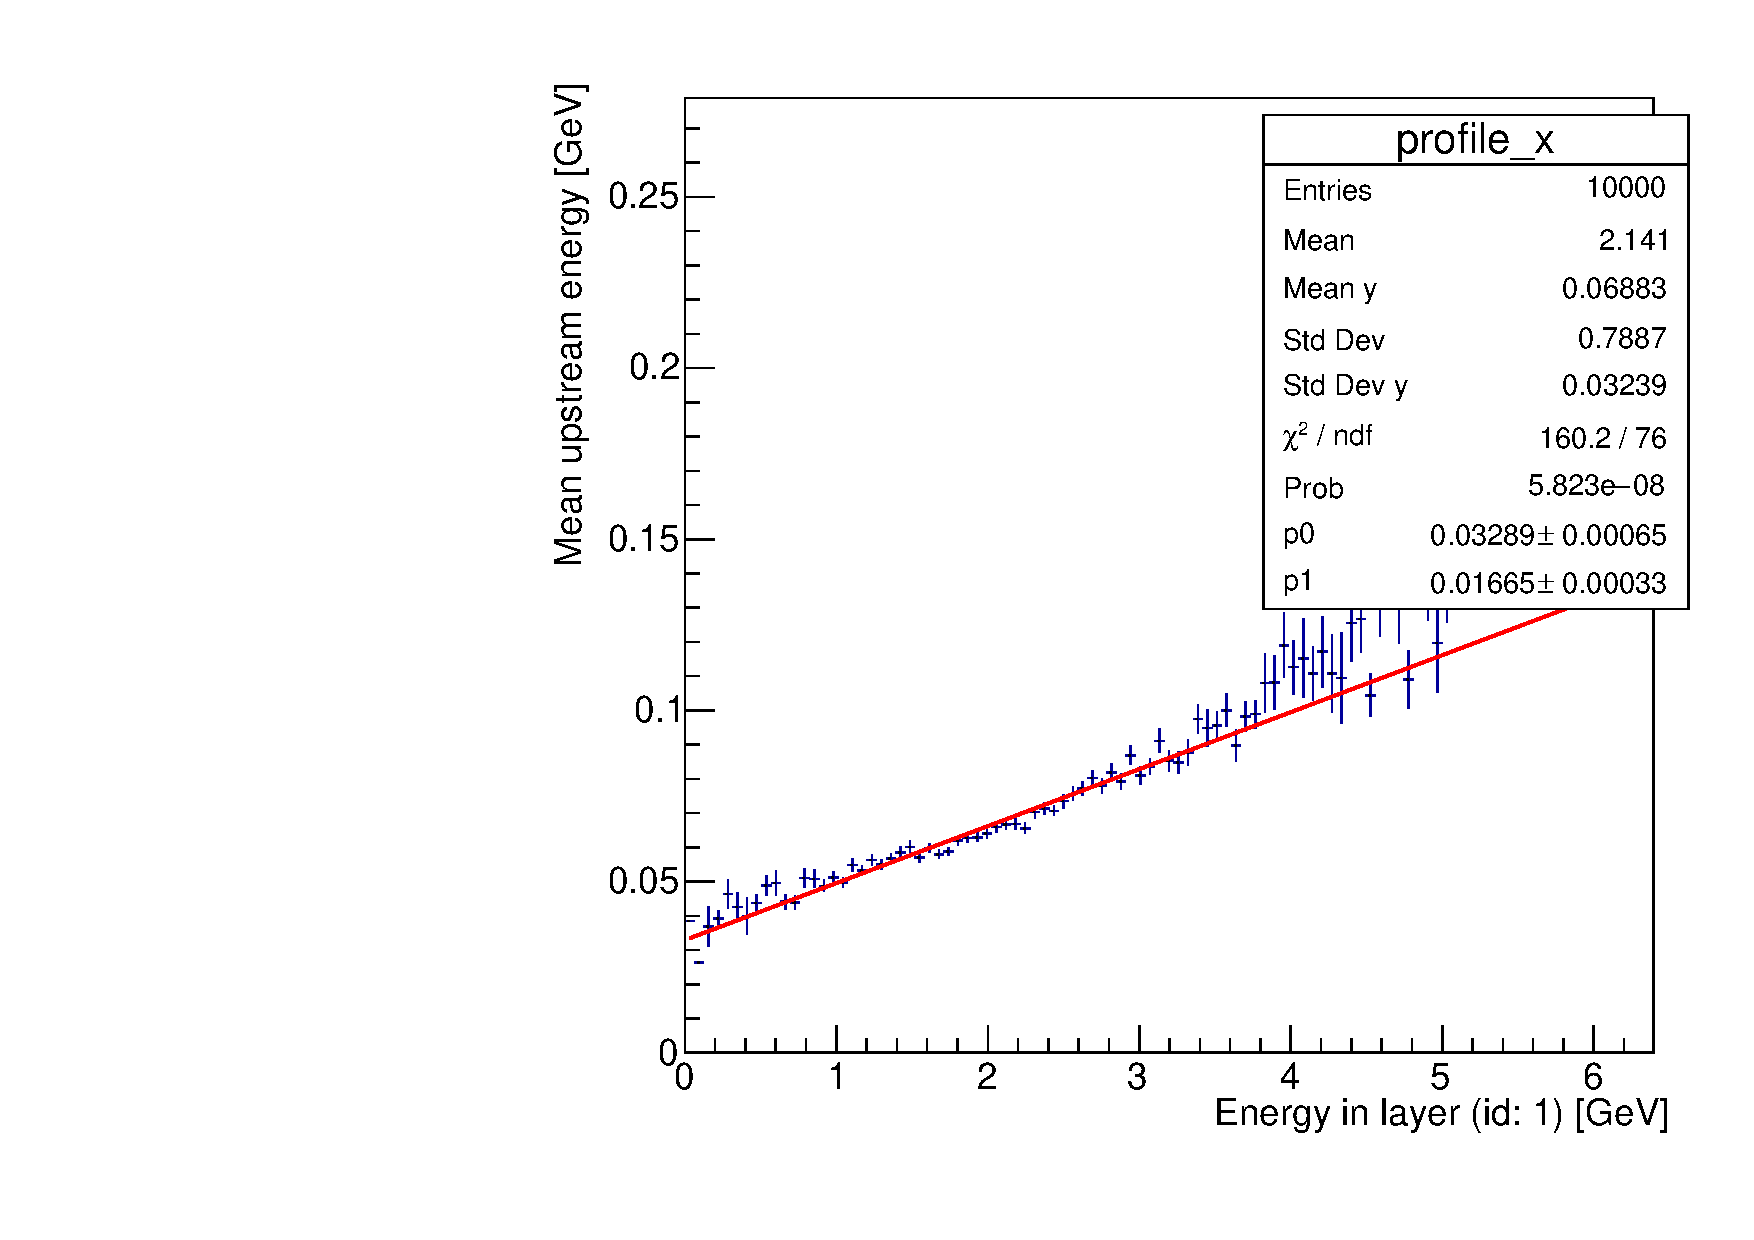
\includegraphics[width=0.39\linewidth]{figures/momentum_id1/profile_upstream_vs_first_layer_90deg_15GeV.pdf}
\end{frame}

\begin{frame}
  \frametitle{At 20 GeV}

  \centering
  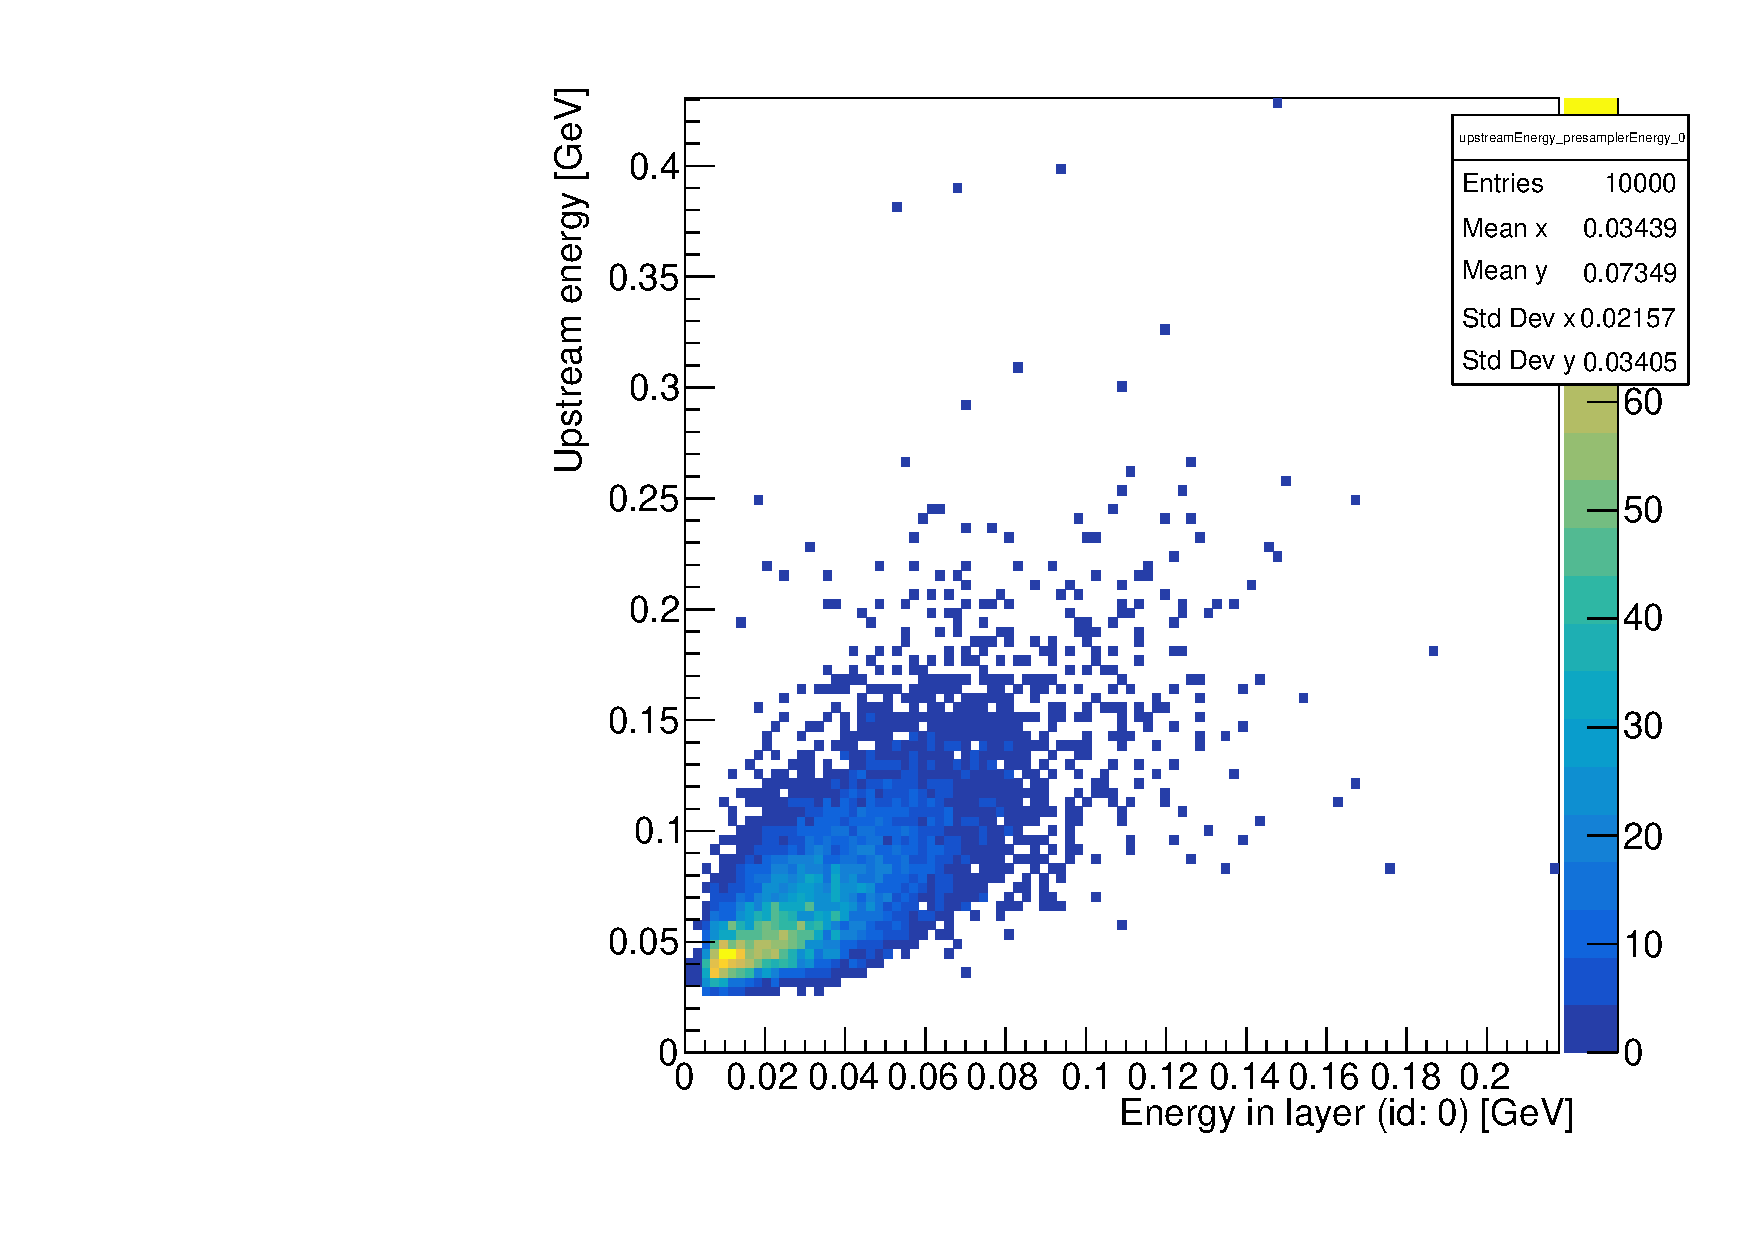
\includegraphics[width=0.39\linewidth]{figures/momentum_id0/hist_upstream_vs_first_layer_90deg_20GeV.pdf}
  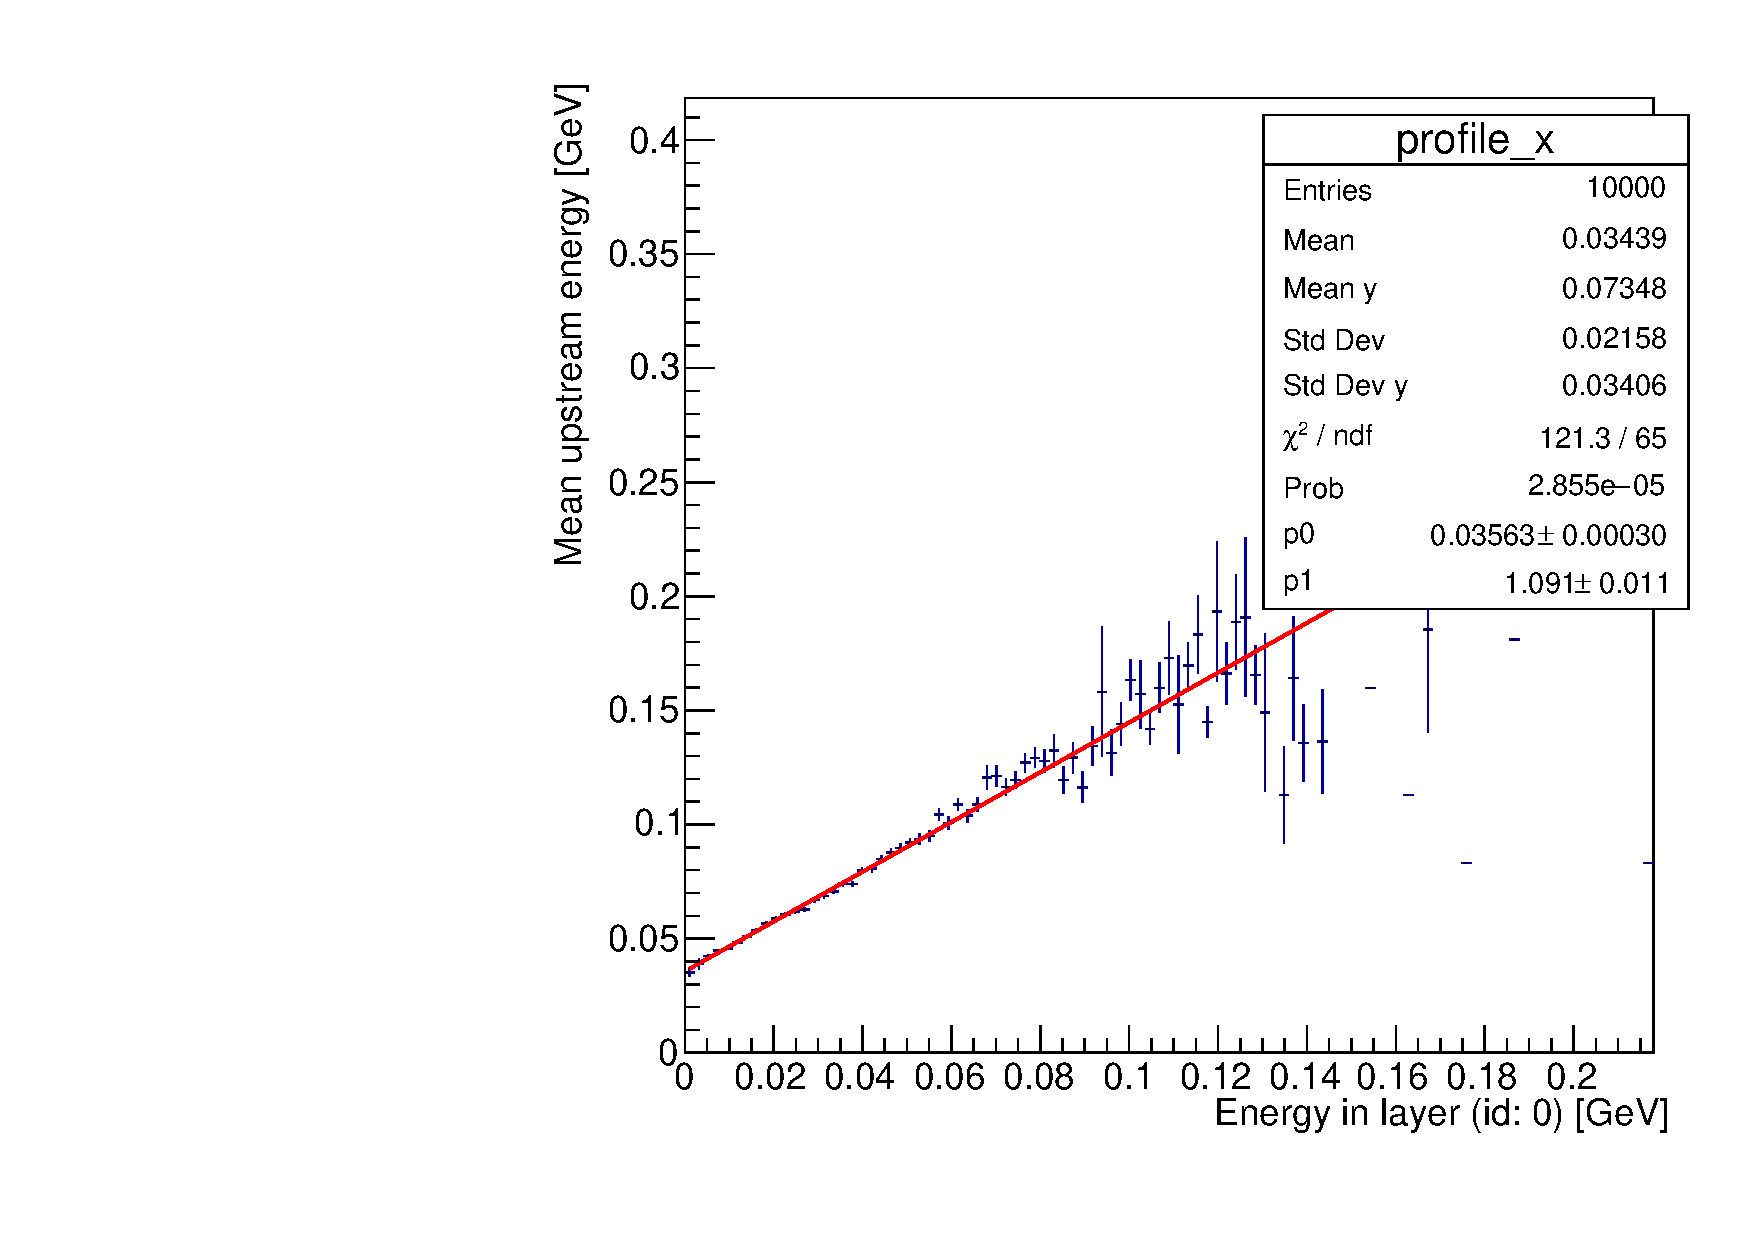
\includegraphics[width=0.39\linewidth]{figures/momentum_id0/profile_upstream_vs_first_layer_90deg_20GeV.pdf} \\
  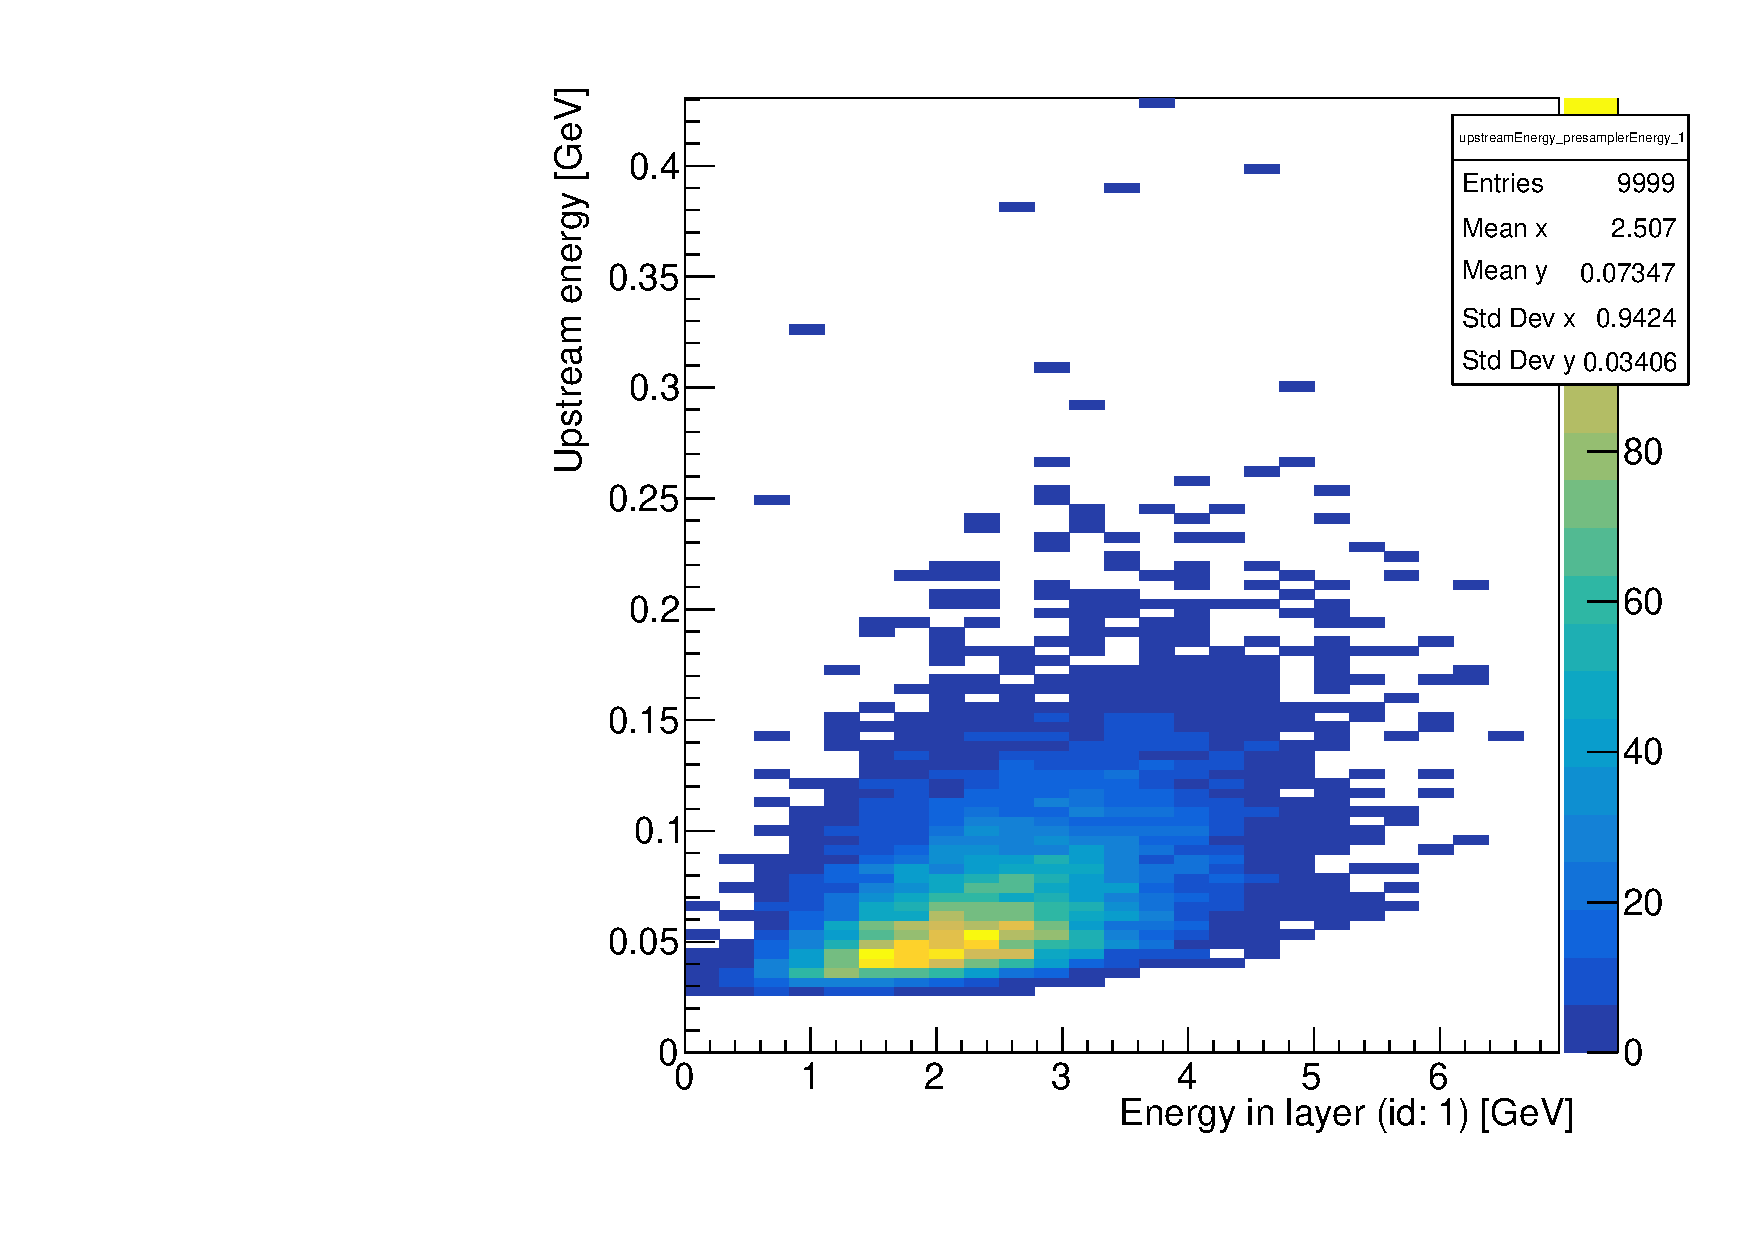
\includegraphics[width=0.39\linewidth]{figures/momentum_id1/hist_upstream_vs_first_layer_90deg_20GeV.pdf}
  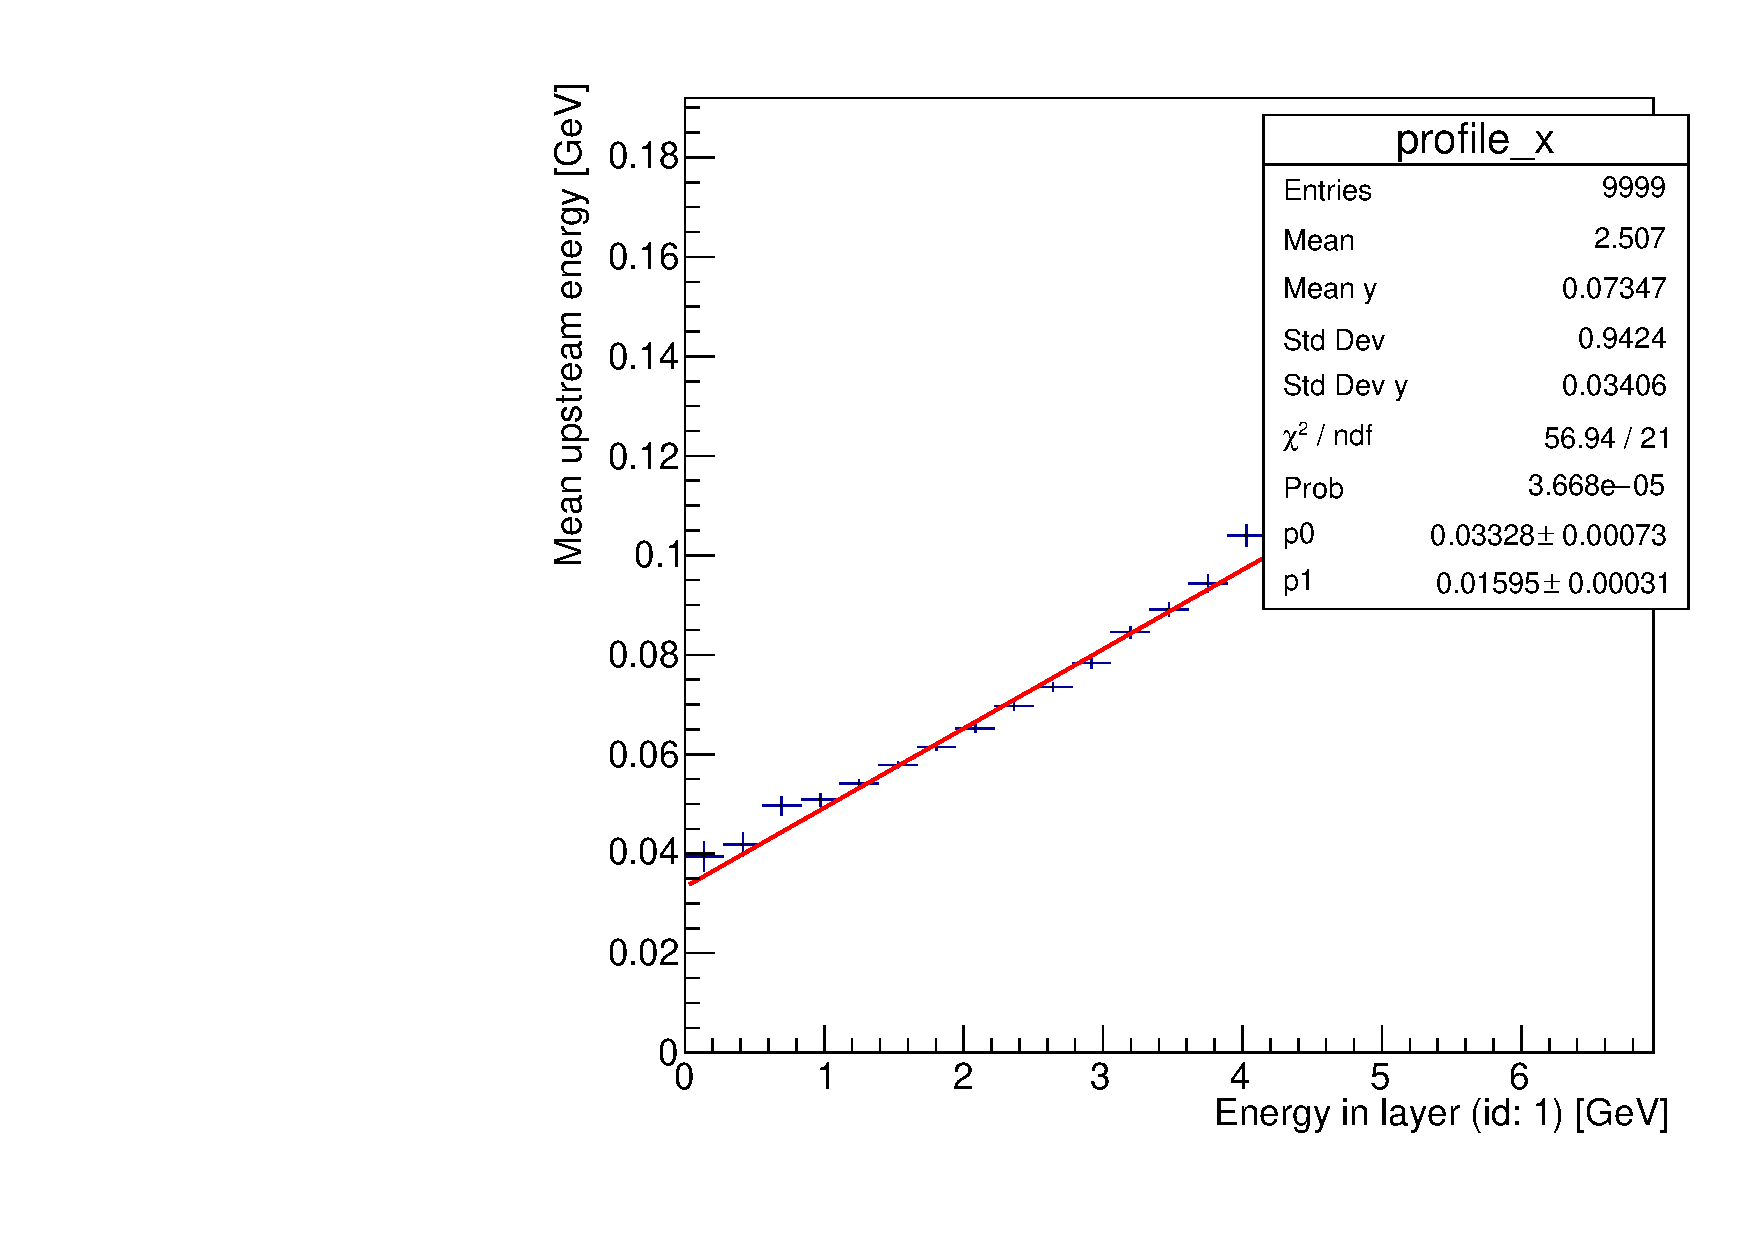
\includegraphics[width=0.39\linewidth]{figures/momentum_id1/profile_upstream_vs_first_layer_90deg_20GeV.pdf}
\end{frame}

\begin{frame}
  \frametitle{At 25 GeV}

  \centering
  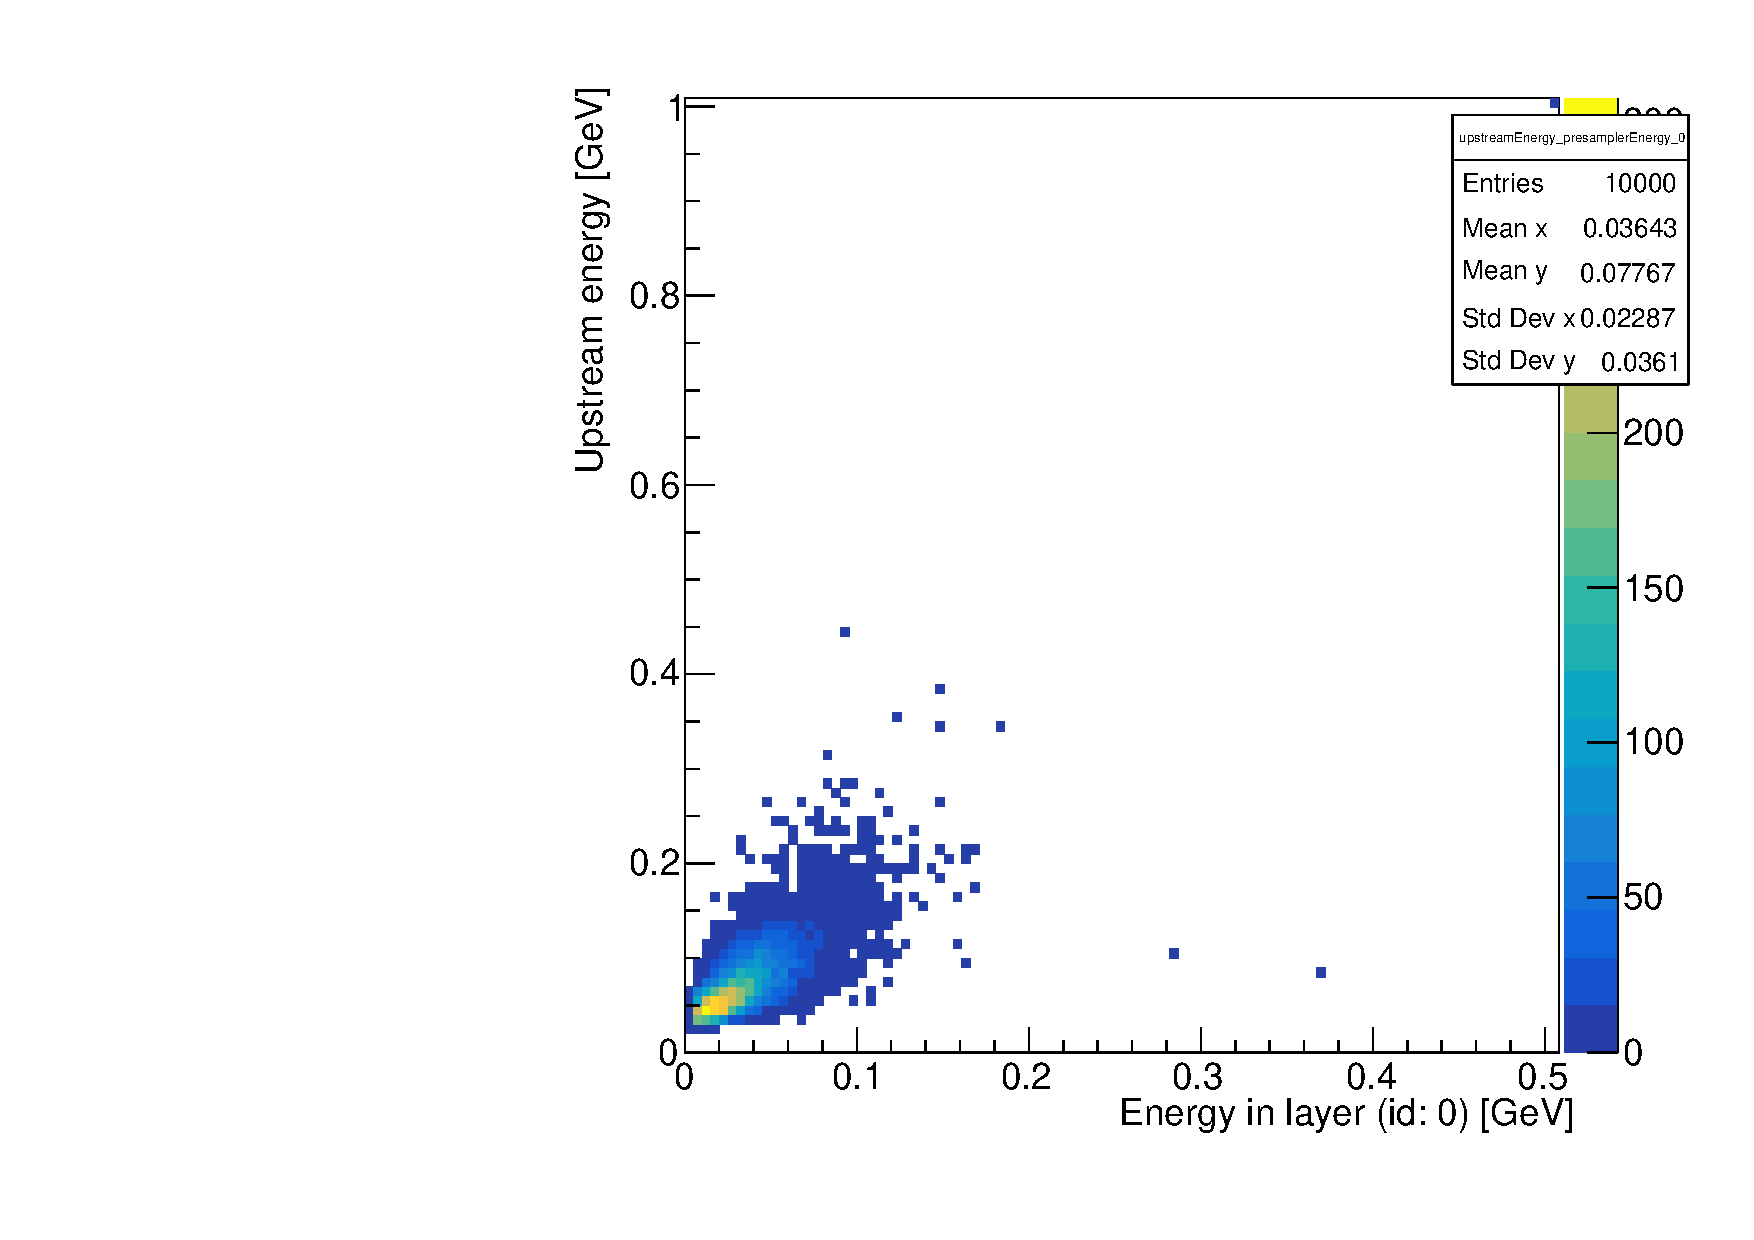
\includegraphics[width=0.39\linewidth]{figures/momentum_id0/hist_upstream_vs_first_layer_90deg_25GeV.pdf}
  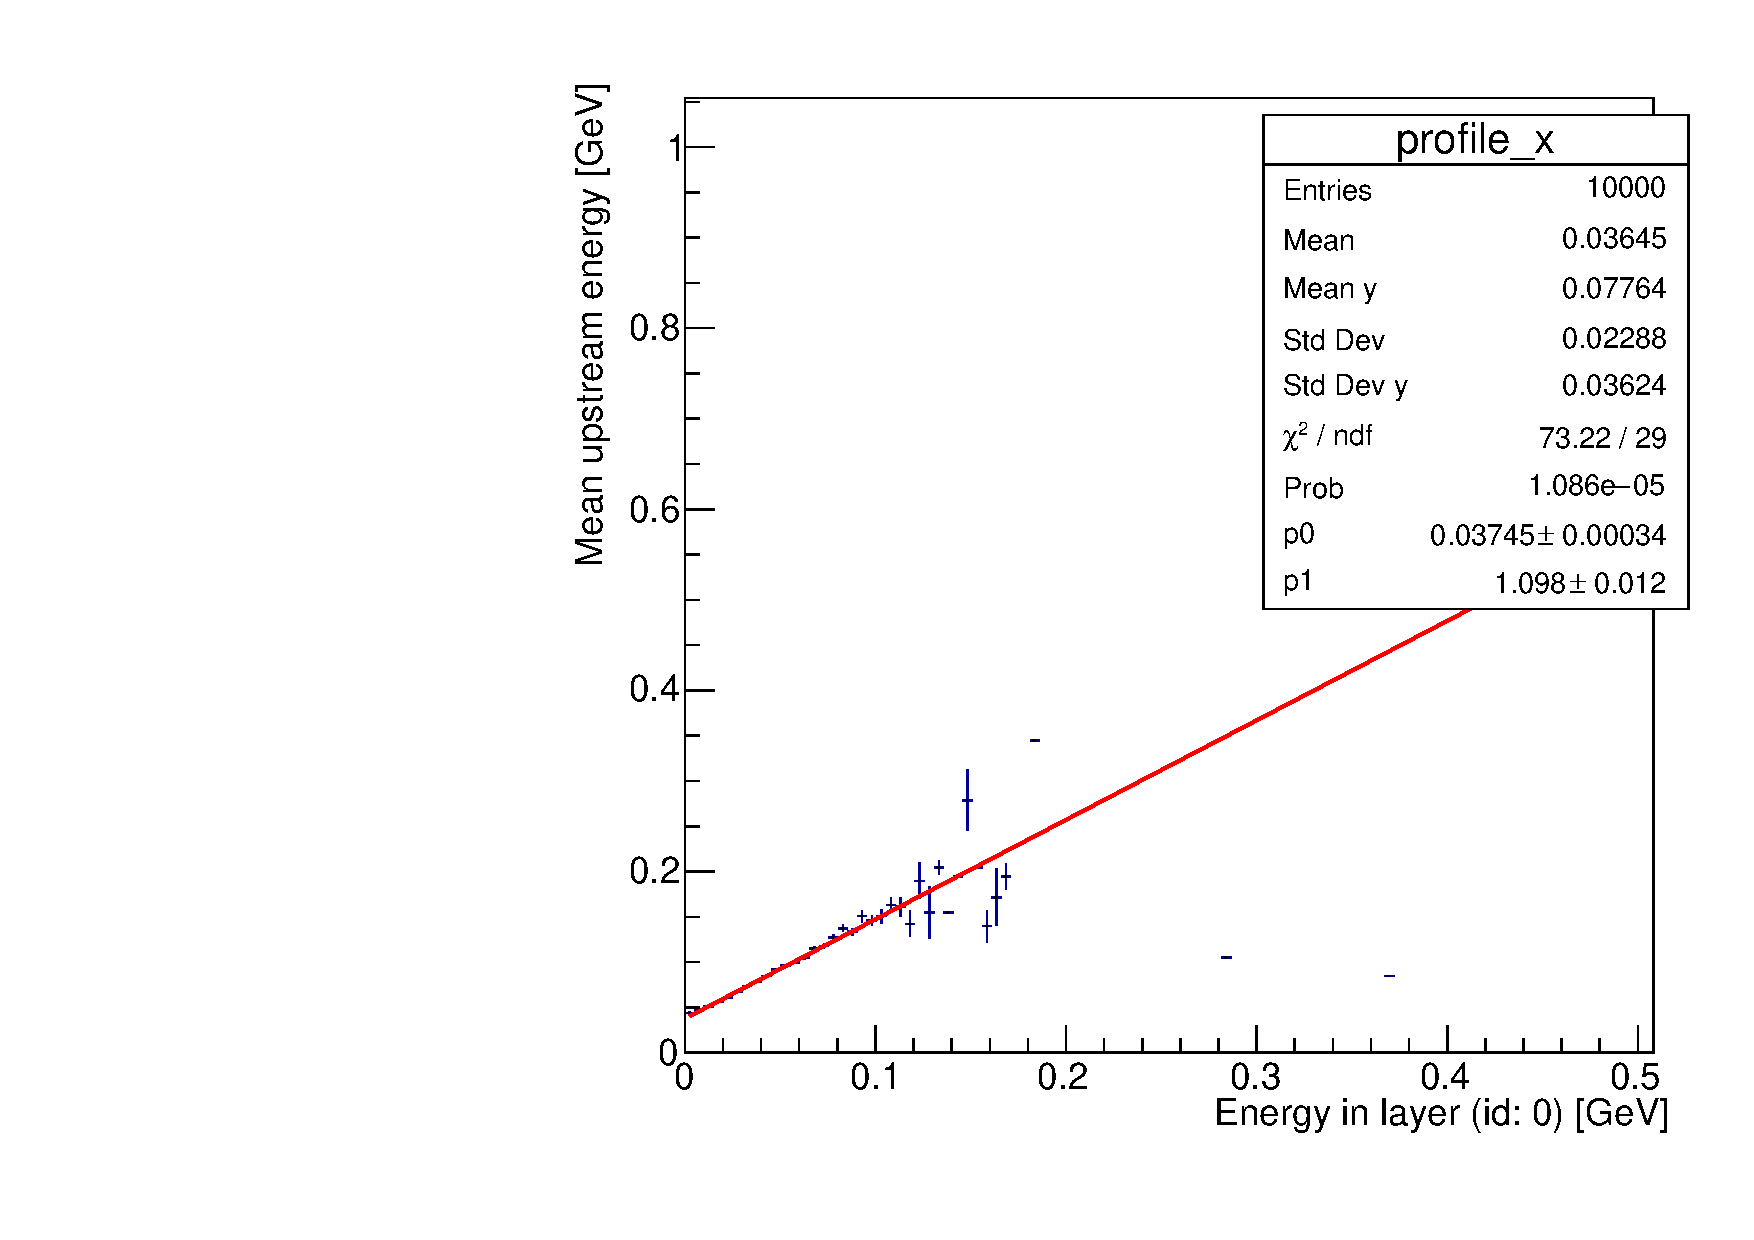
\includegraphics[width=0.39\linewidth]{figures/momentum_id0/profile_upstream_vs_first_layer_90deg_25GeV.pdf} \\
  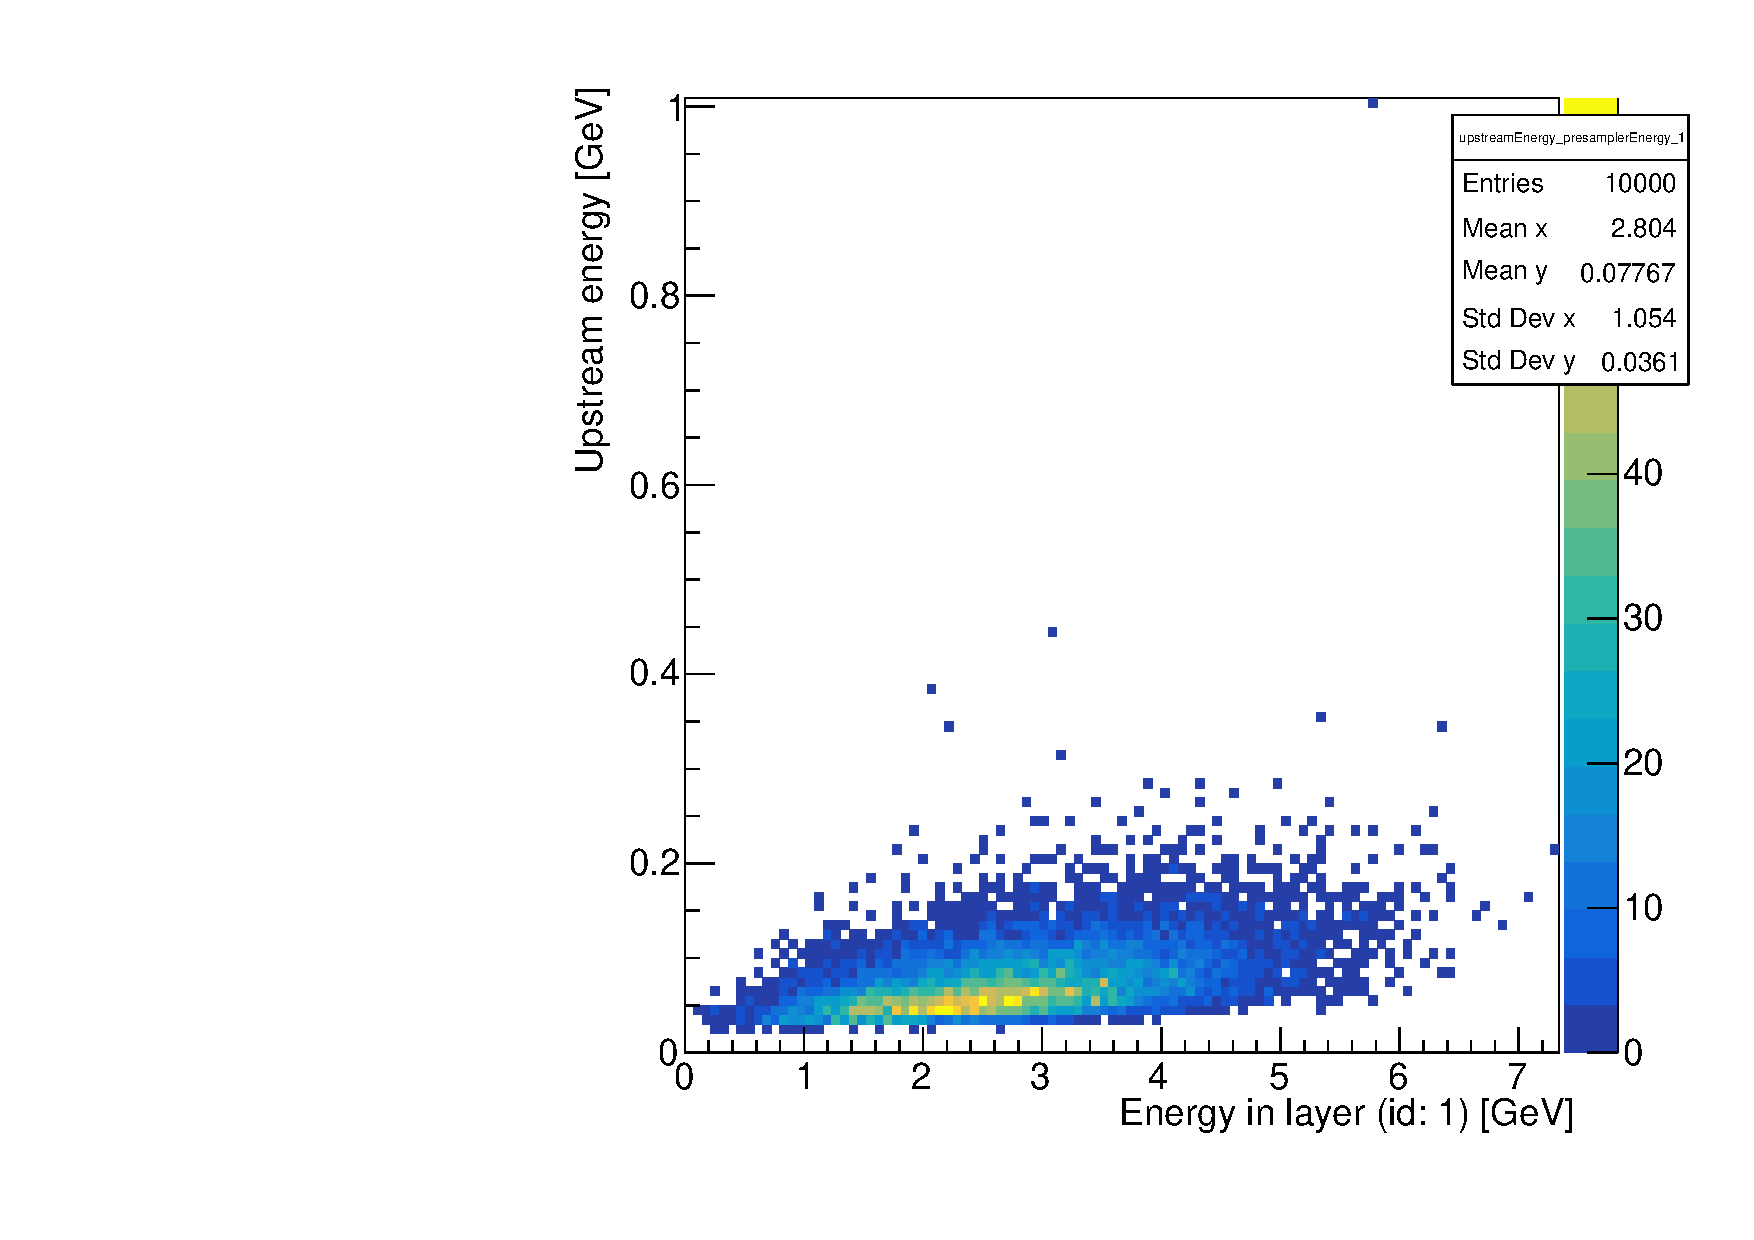
\includegraphics[width=0.39\linewidth]{figures/momentum_id1/hist_upstream_vs_first_layer_90deg_25GeV.pdf}
  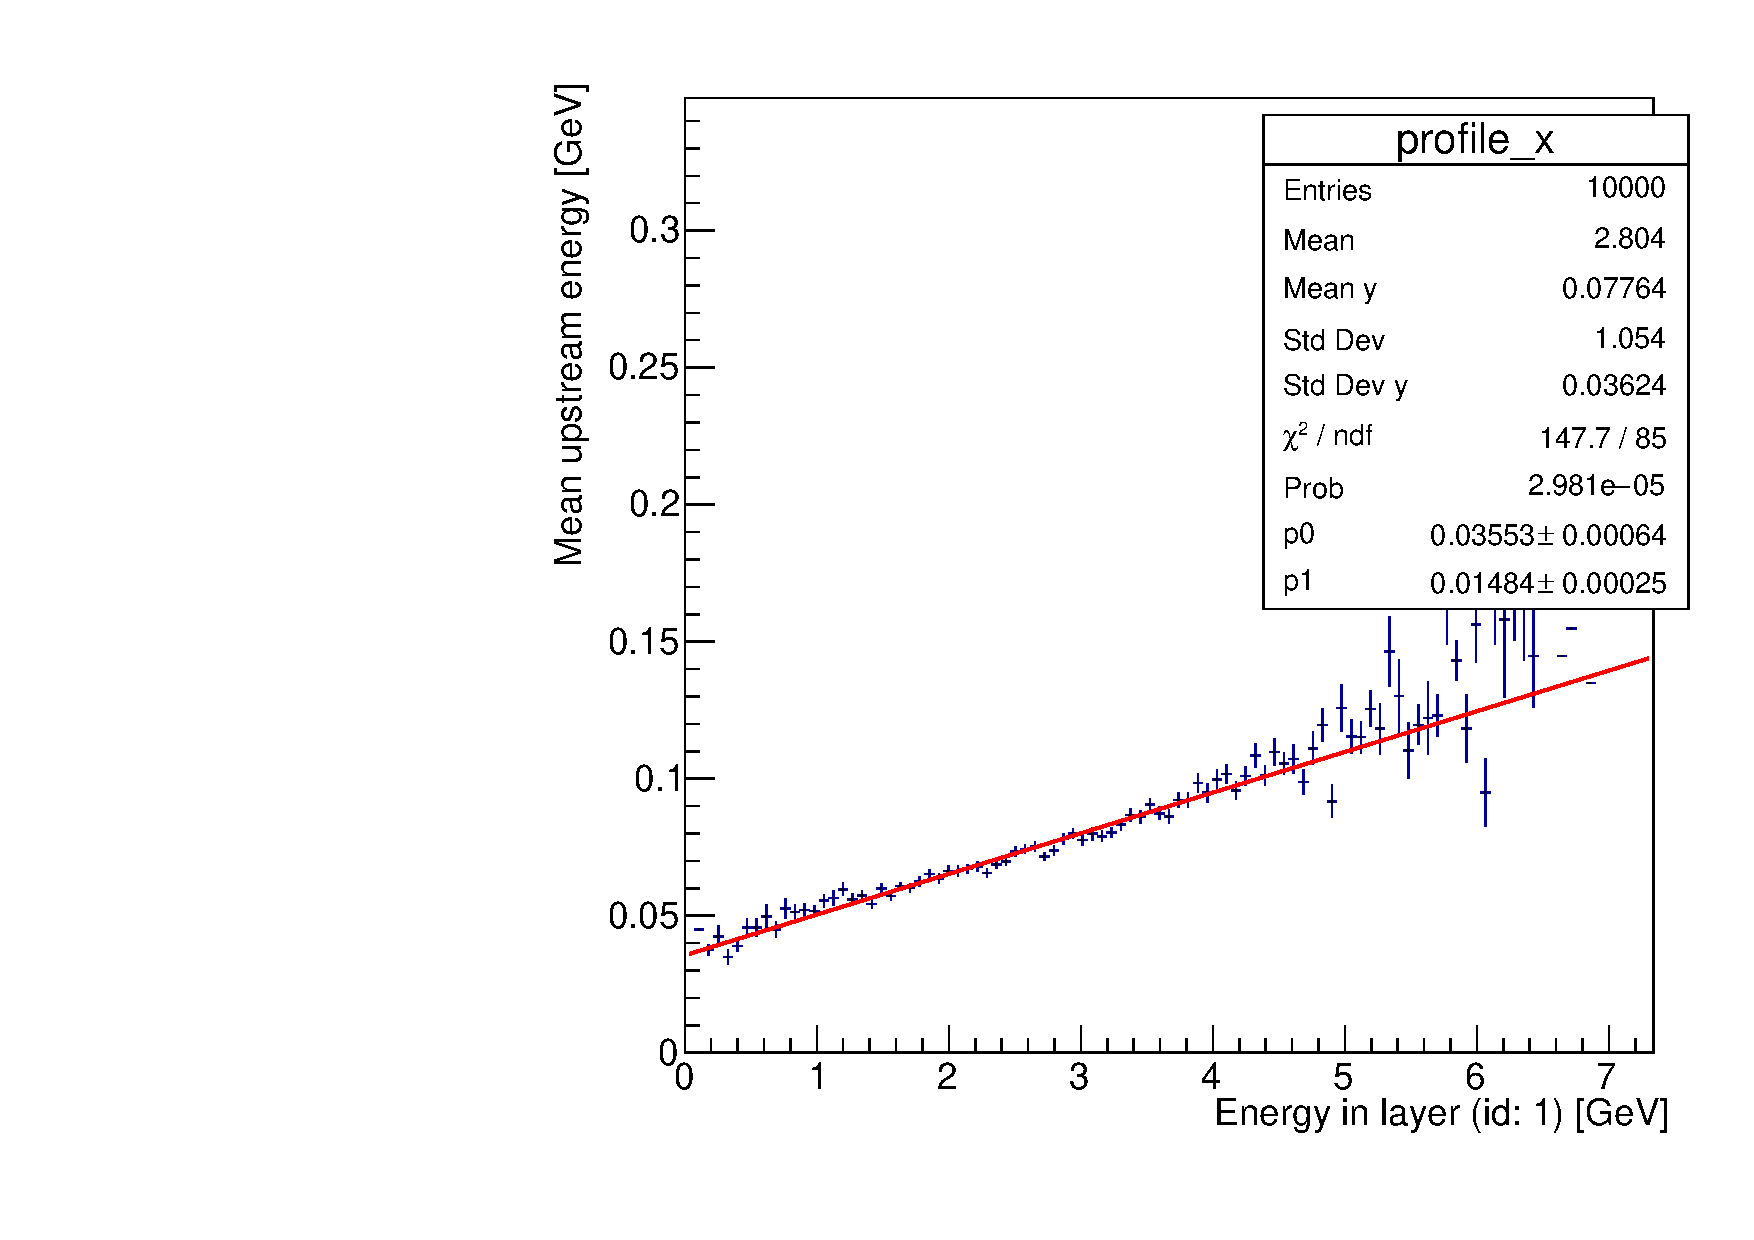
\includegraphics[width=0.39\linewidth]{figures/momentum_id1/profile_upstream_vs_first_layer_90deg_25GeV.pdf}
\end{frame}

\begin{frame}
  \frametitle{At 30 GeV}

  \centering
  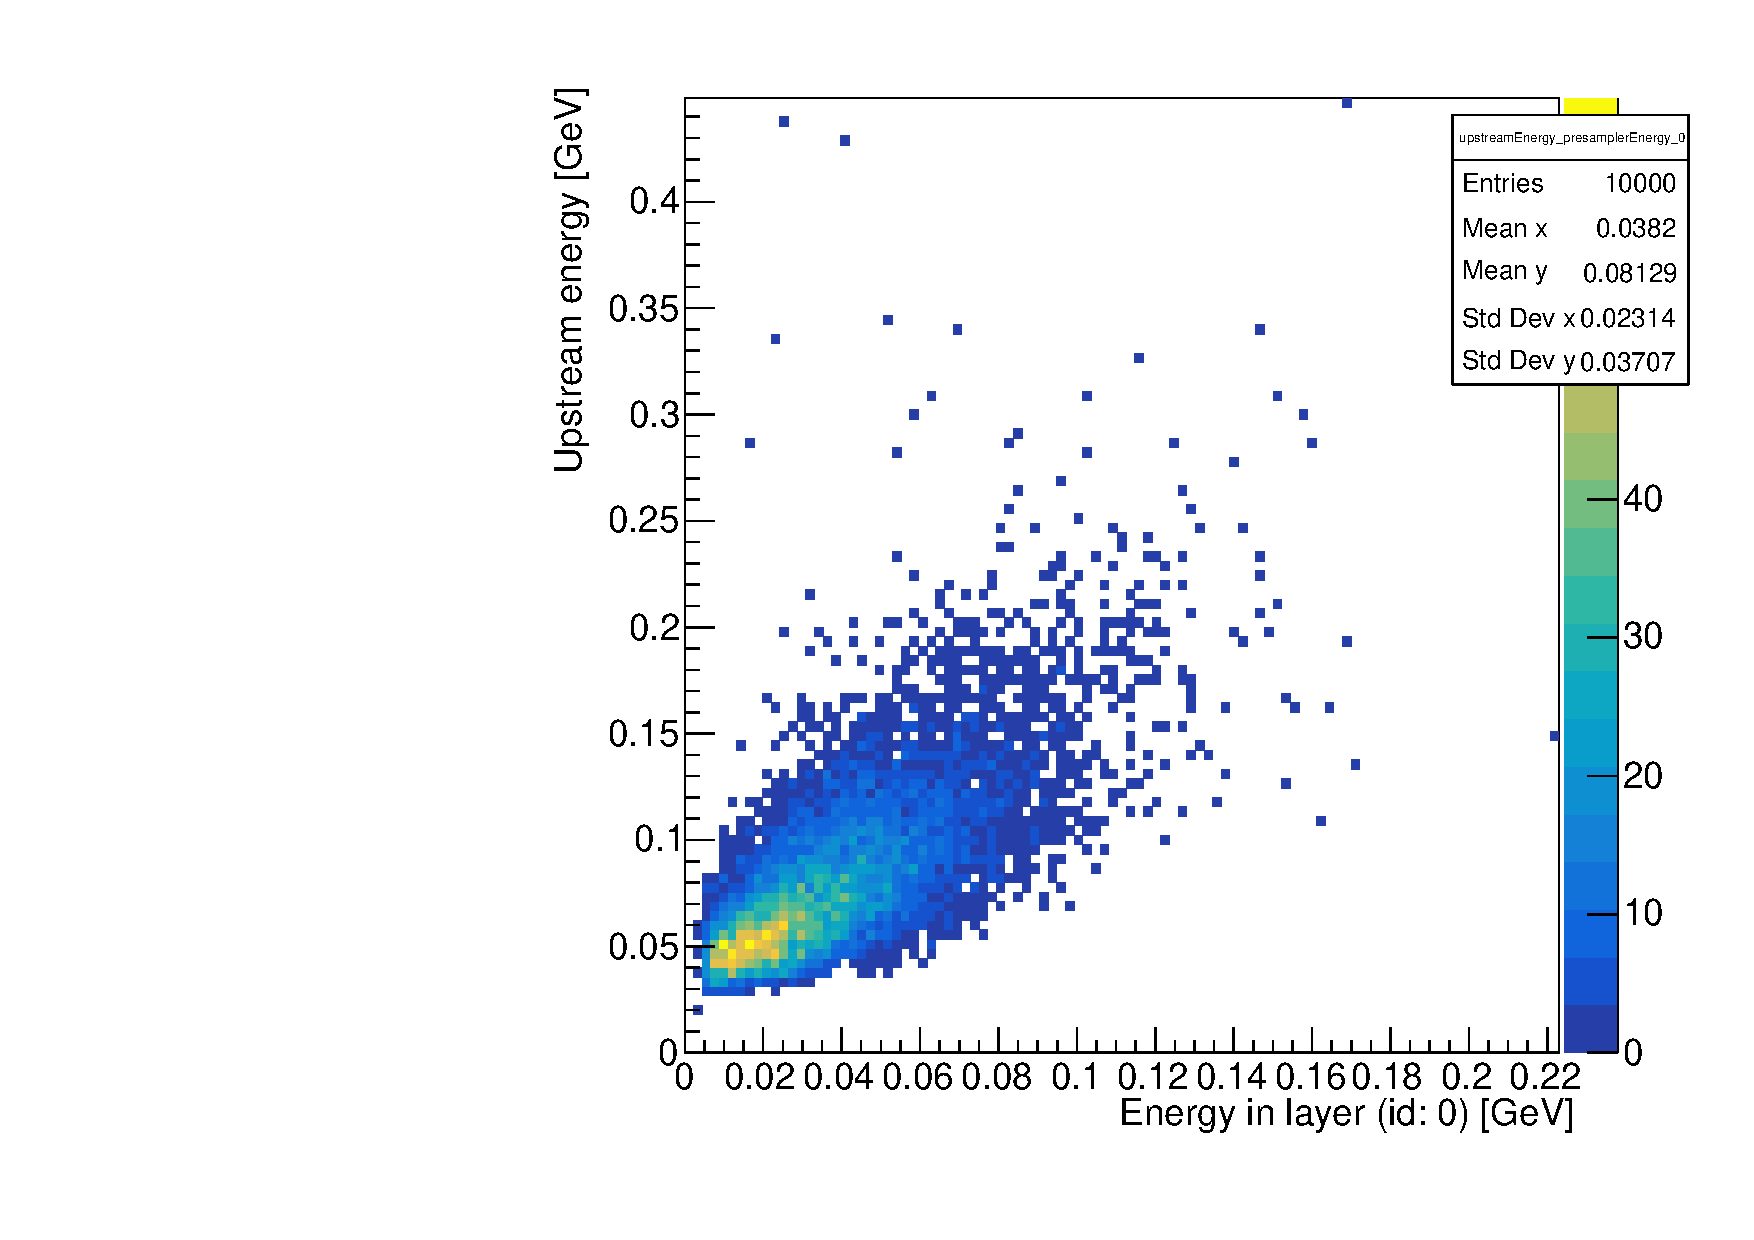
\includegraphics[width=0.39\linewidth]{figures/momentum_id0/hist_upstream_vs_first_layer_90deg_30GeV.pdf}
  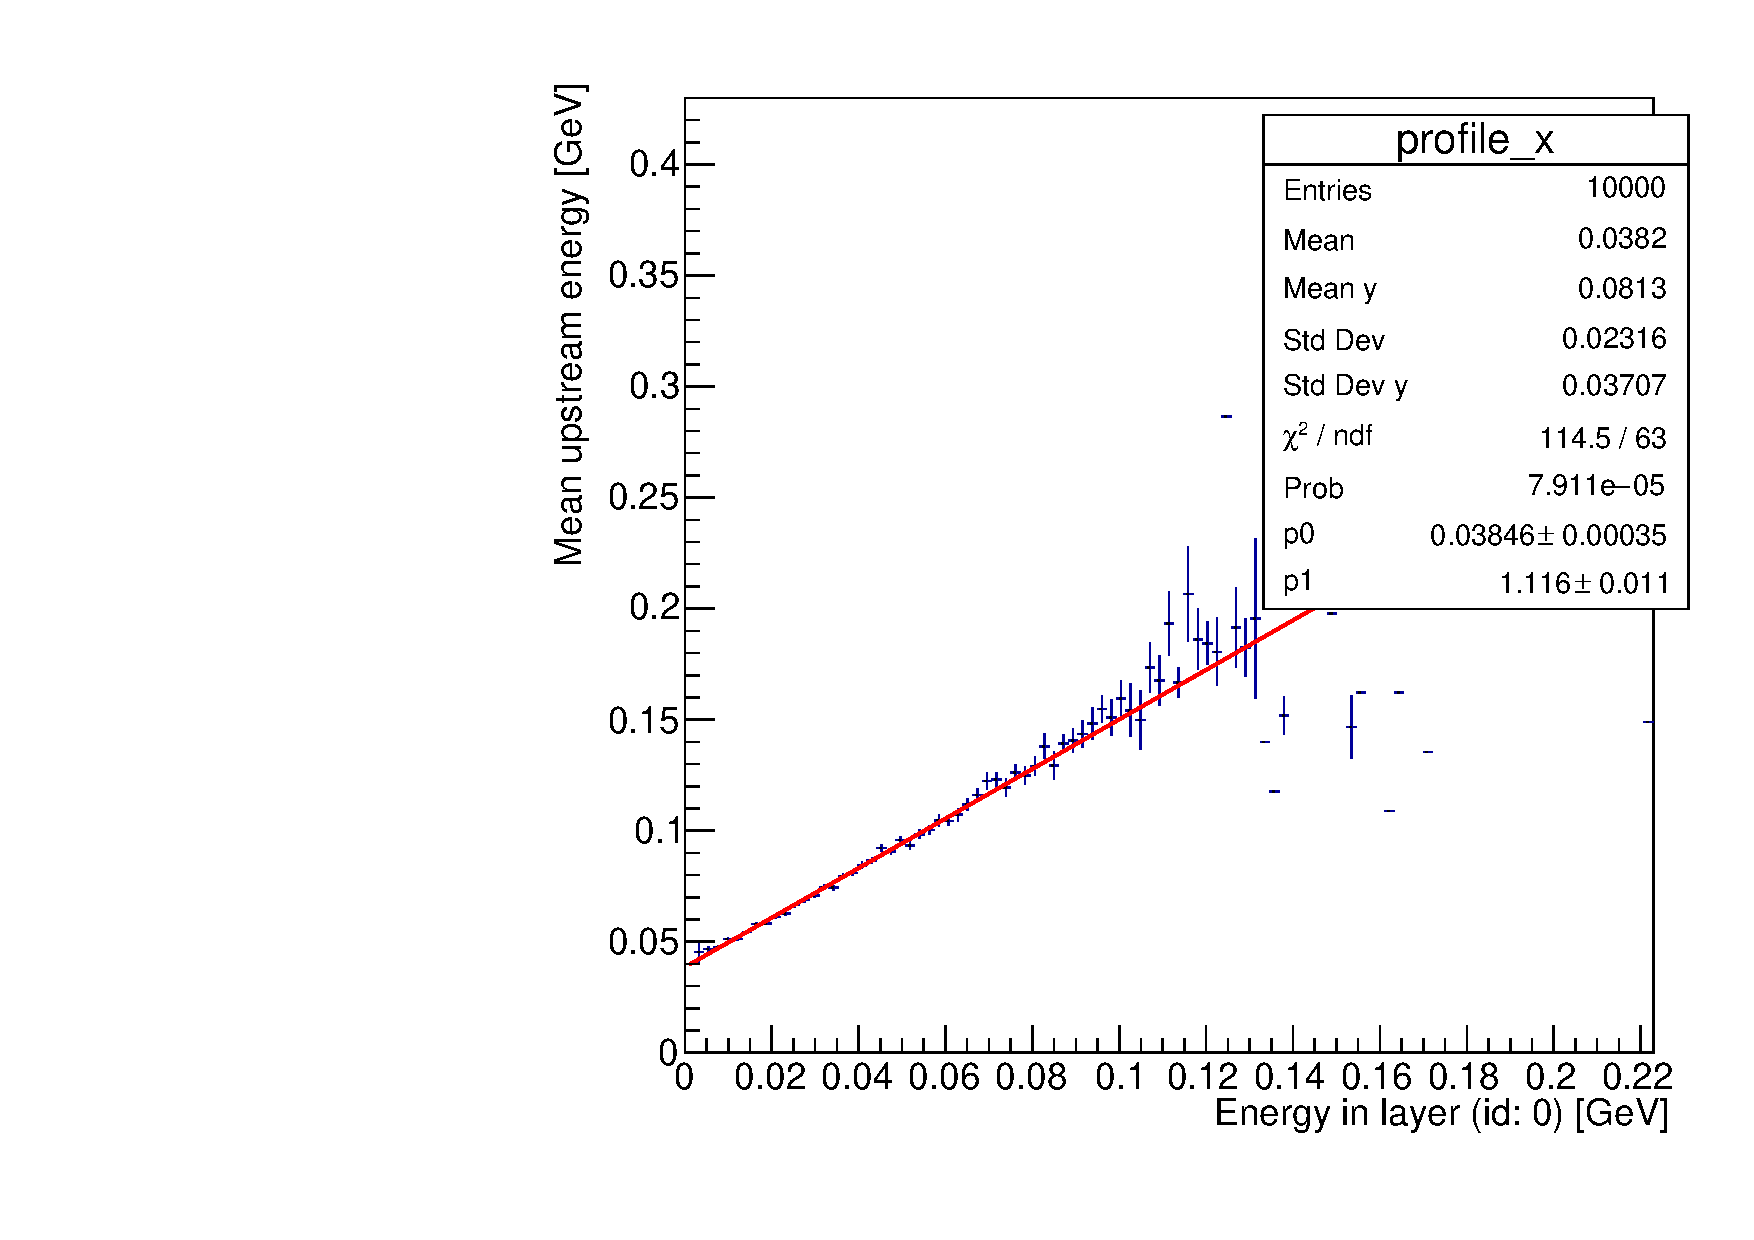
\includegraphics[width=0.39\linewidth]{figures/momentum_id0/profile_upstream_vs_first_layer_90deg_30GeV.pdf} \\
  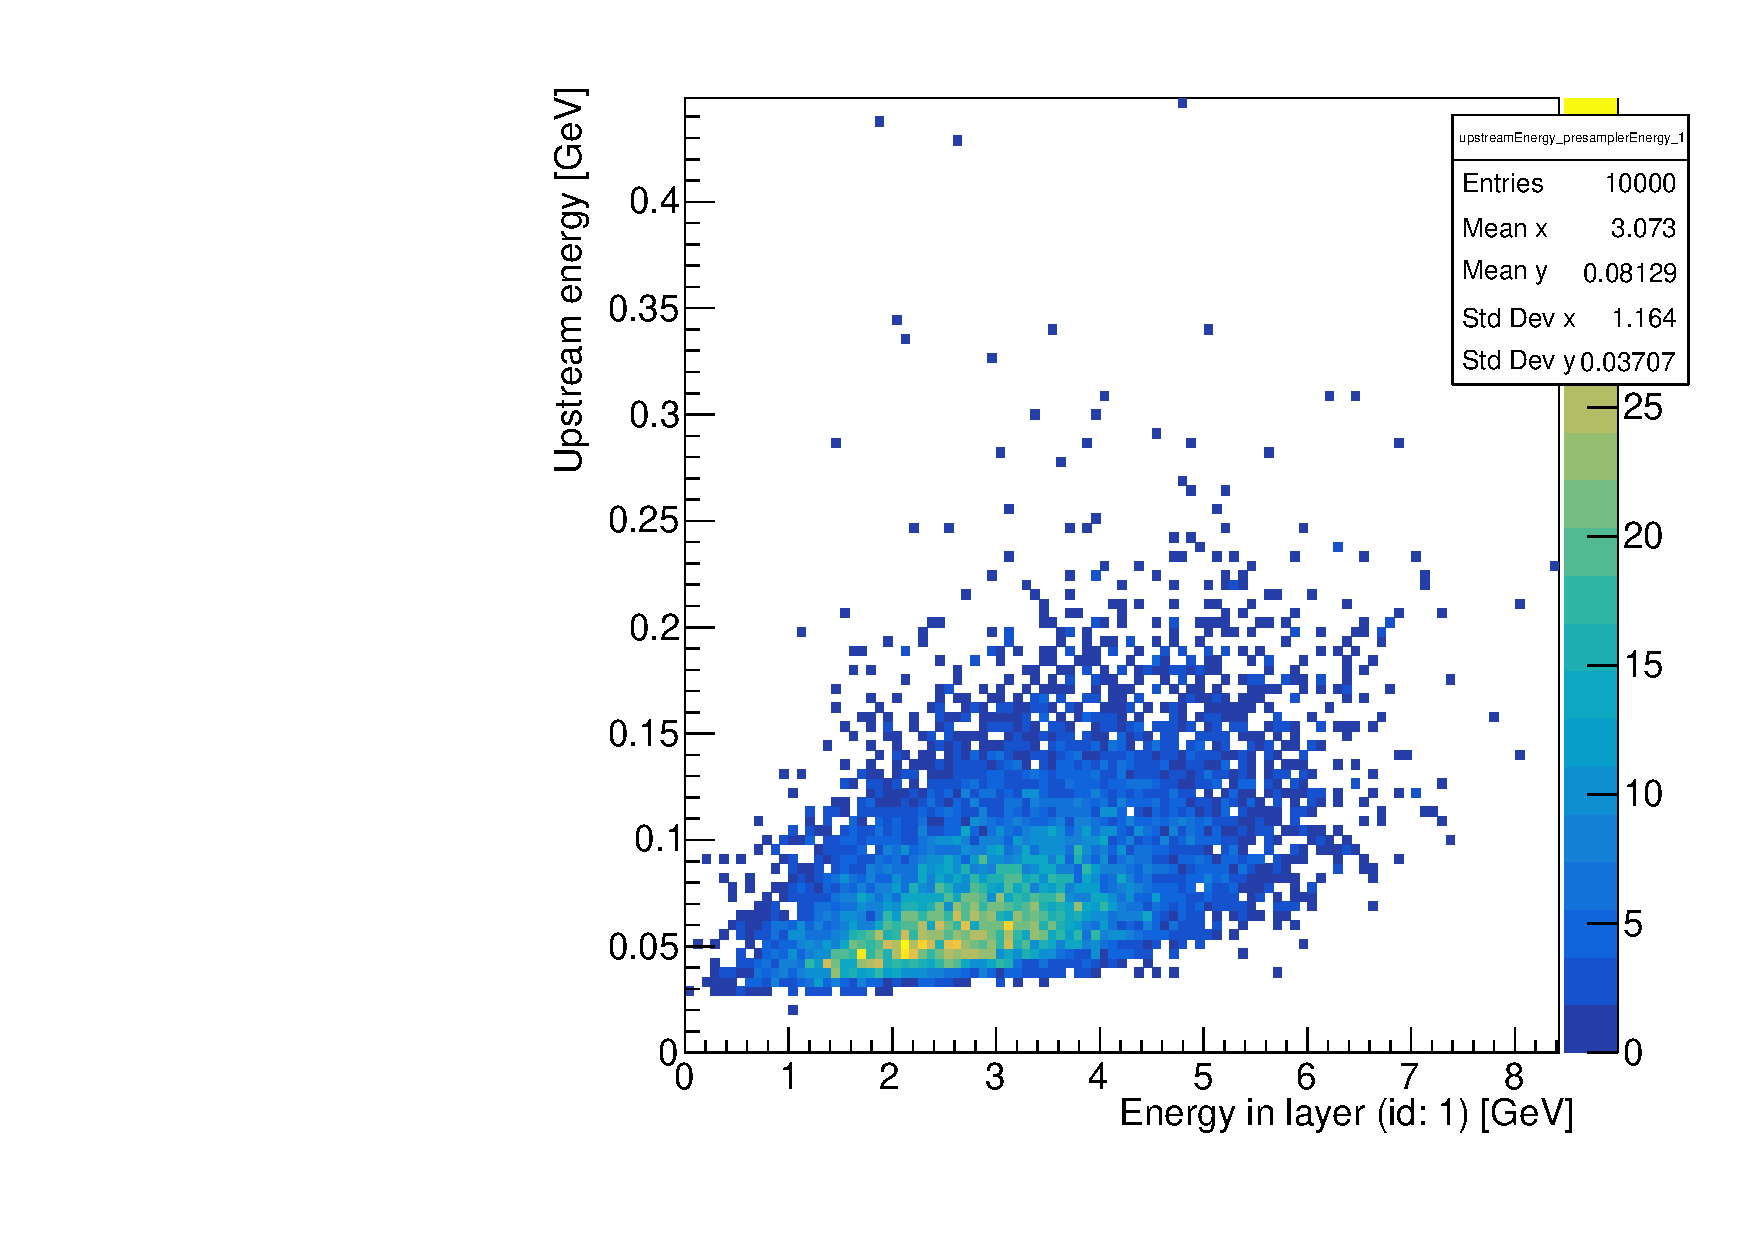
\includegraphics[width=0.39\linewidth]{figures/momentum_id1/hist_upstream_vs_first_layer_90deg_30GeV.pdf}
  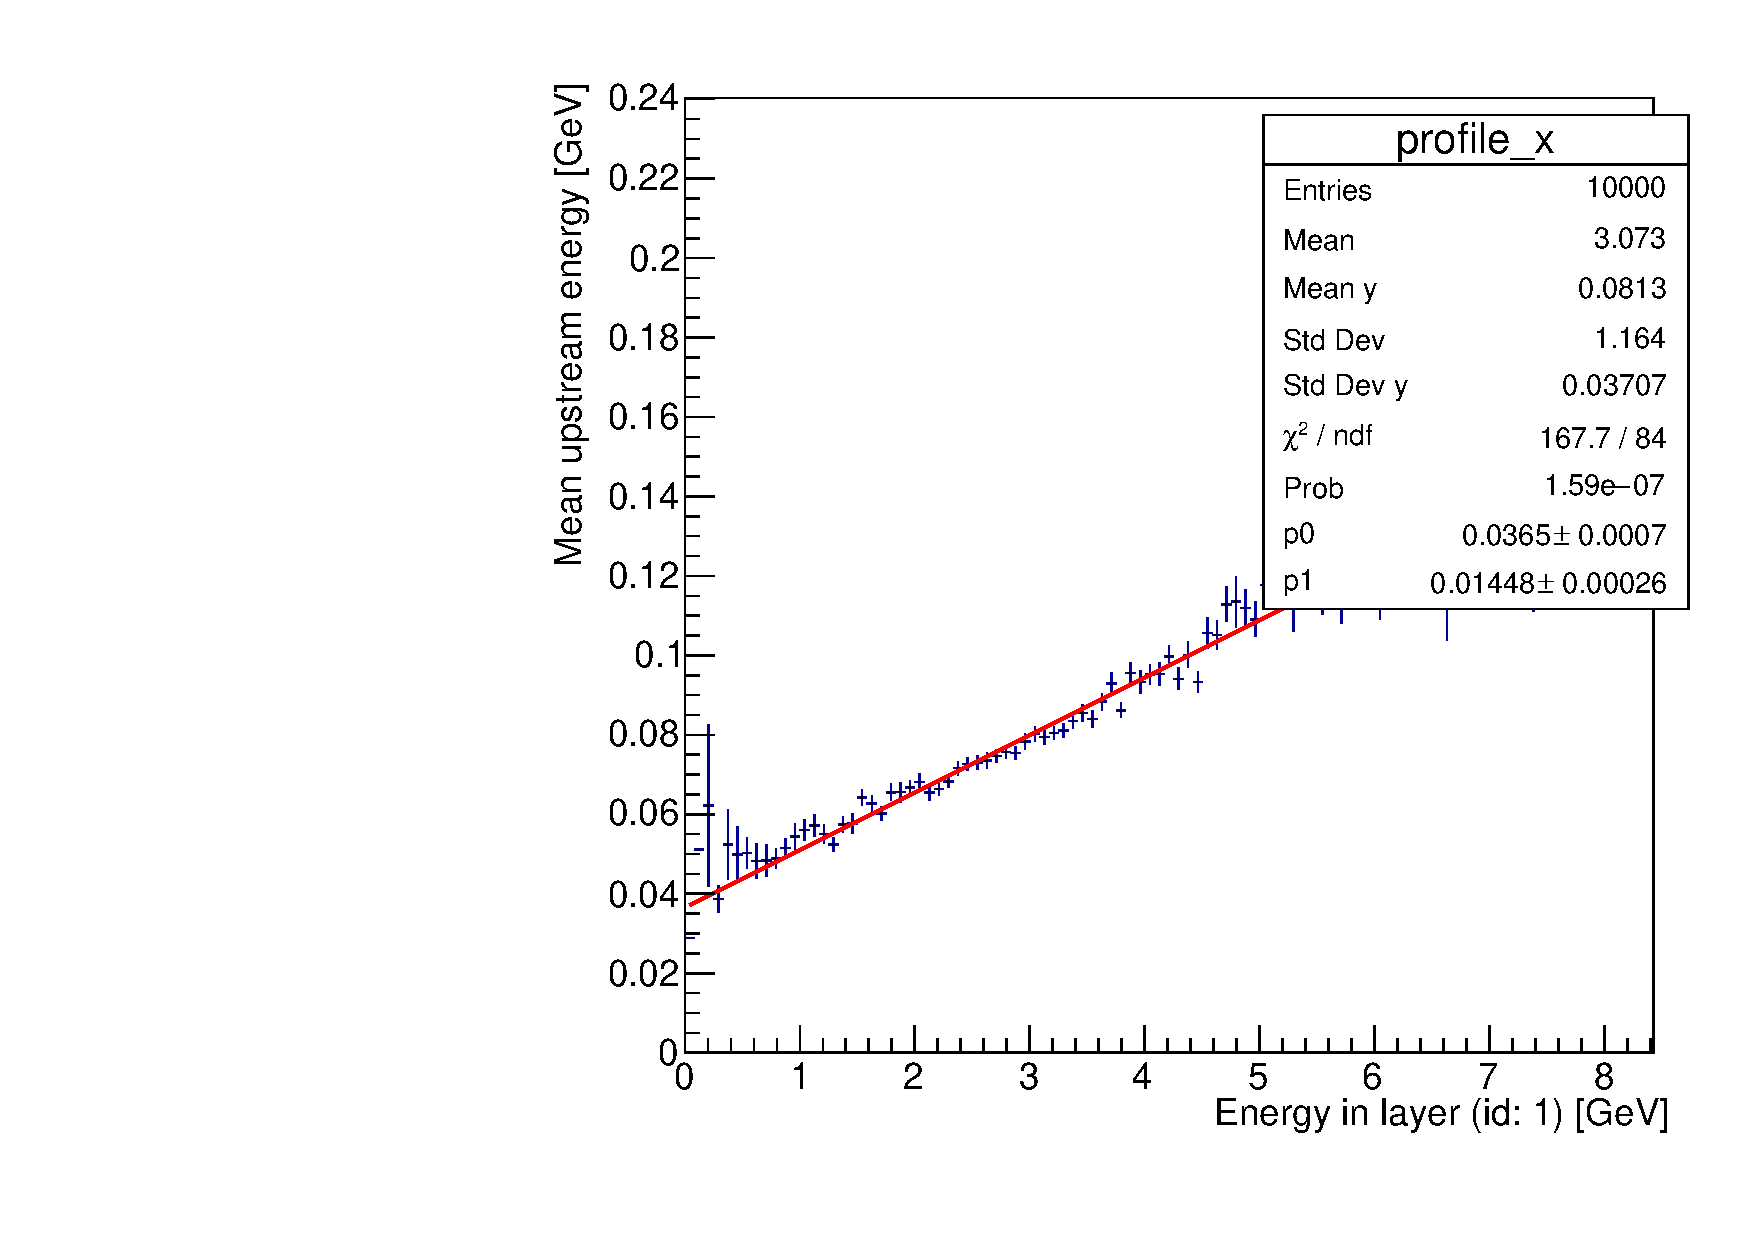
\includegraphics[width=0.39\linewidth]{figures/momentum_id1/profile_upstream_vs_first_layer_90deg_30GeV.pdf}
\end{frame}

\begin{frame}
  \frametitle{At 50 GeV}

  \centering
  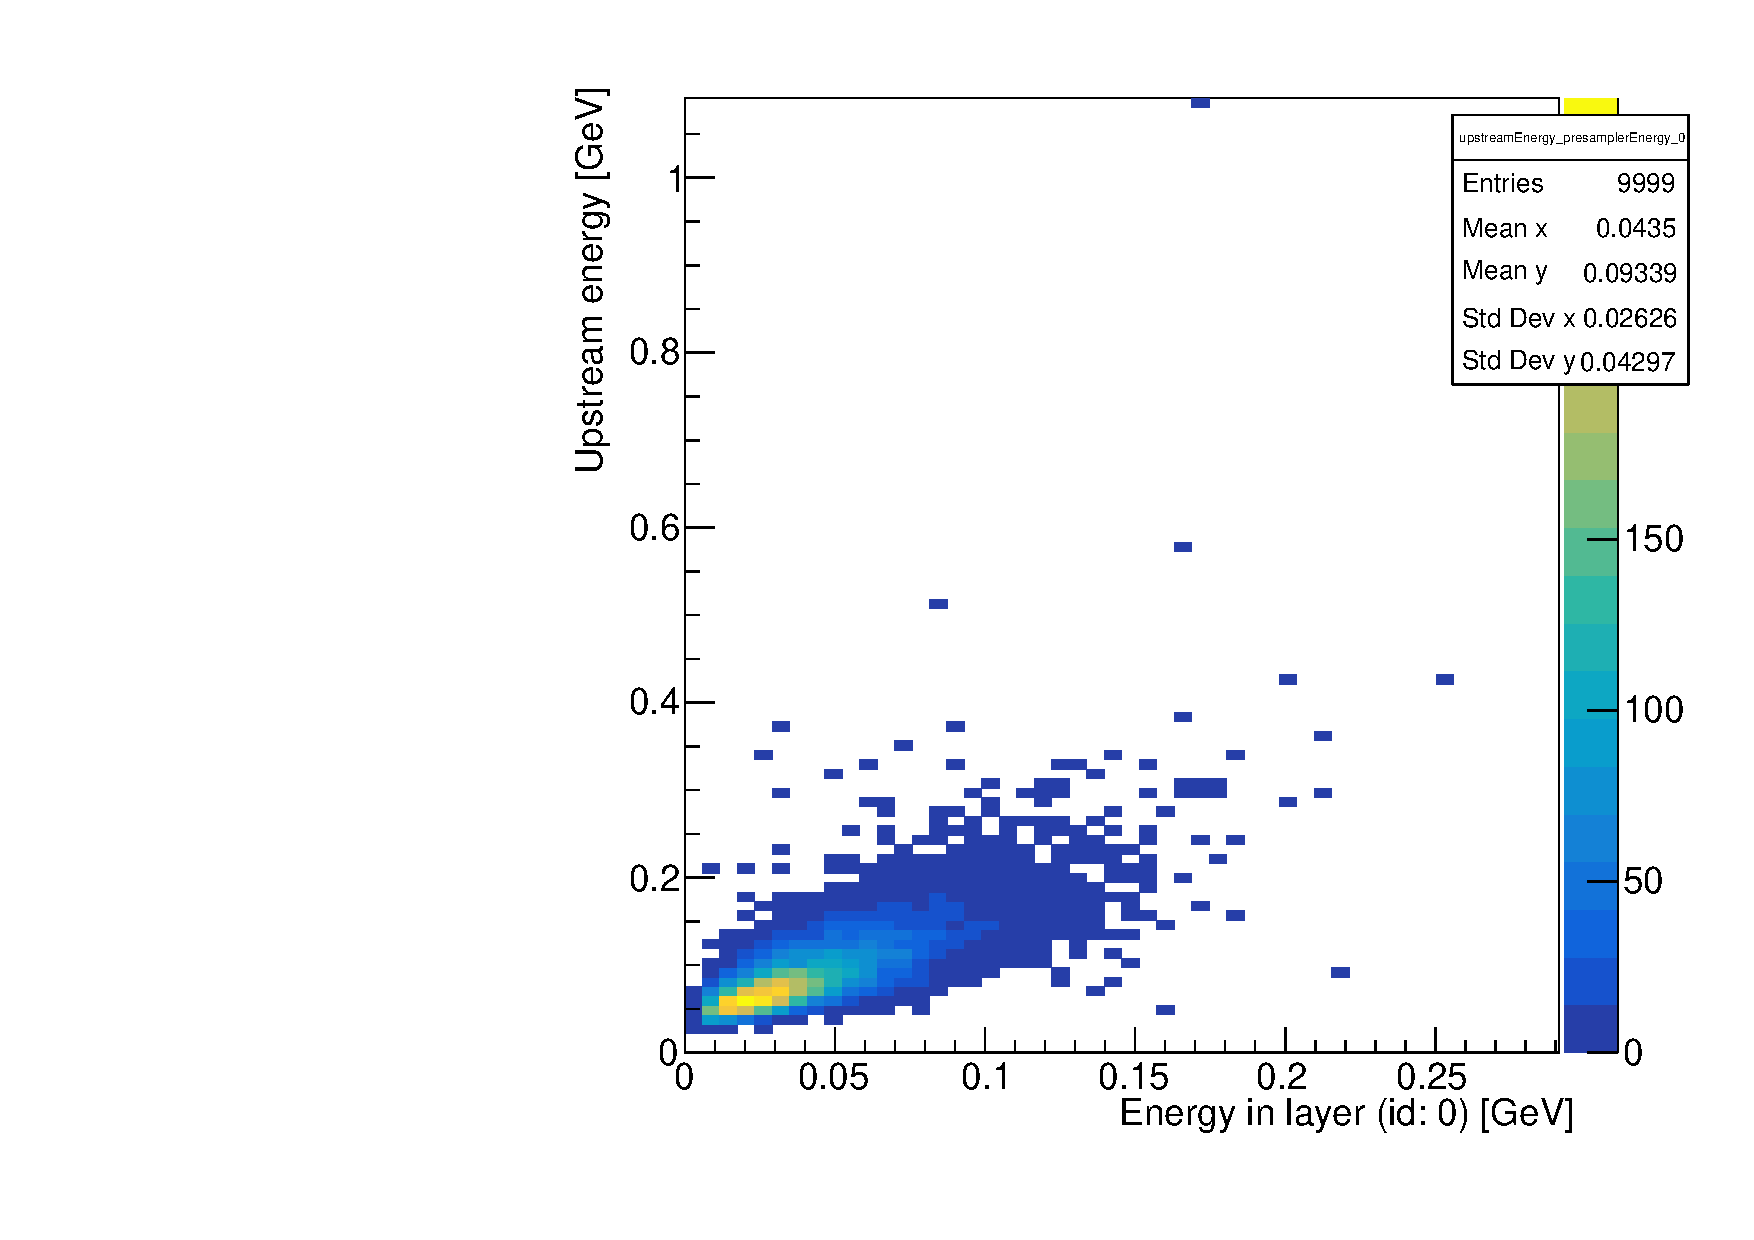
\includegraphics[width=0.39\linewidth]{figures/momentum_id0/hist_upstream_vs_first_layer_90deg_50GeV.pdf}
  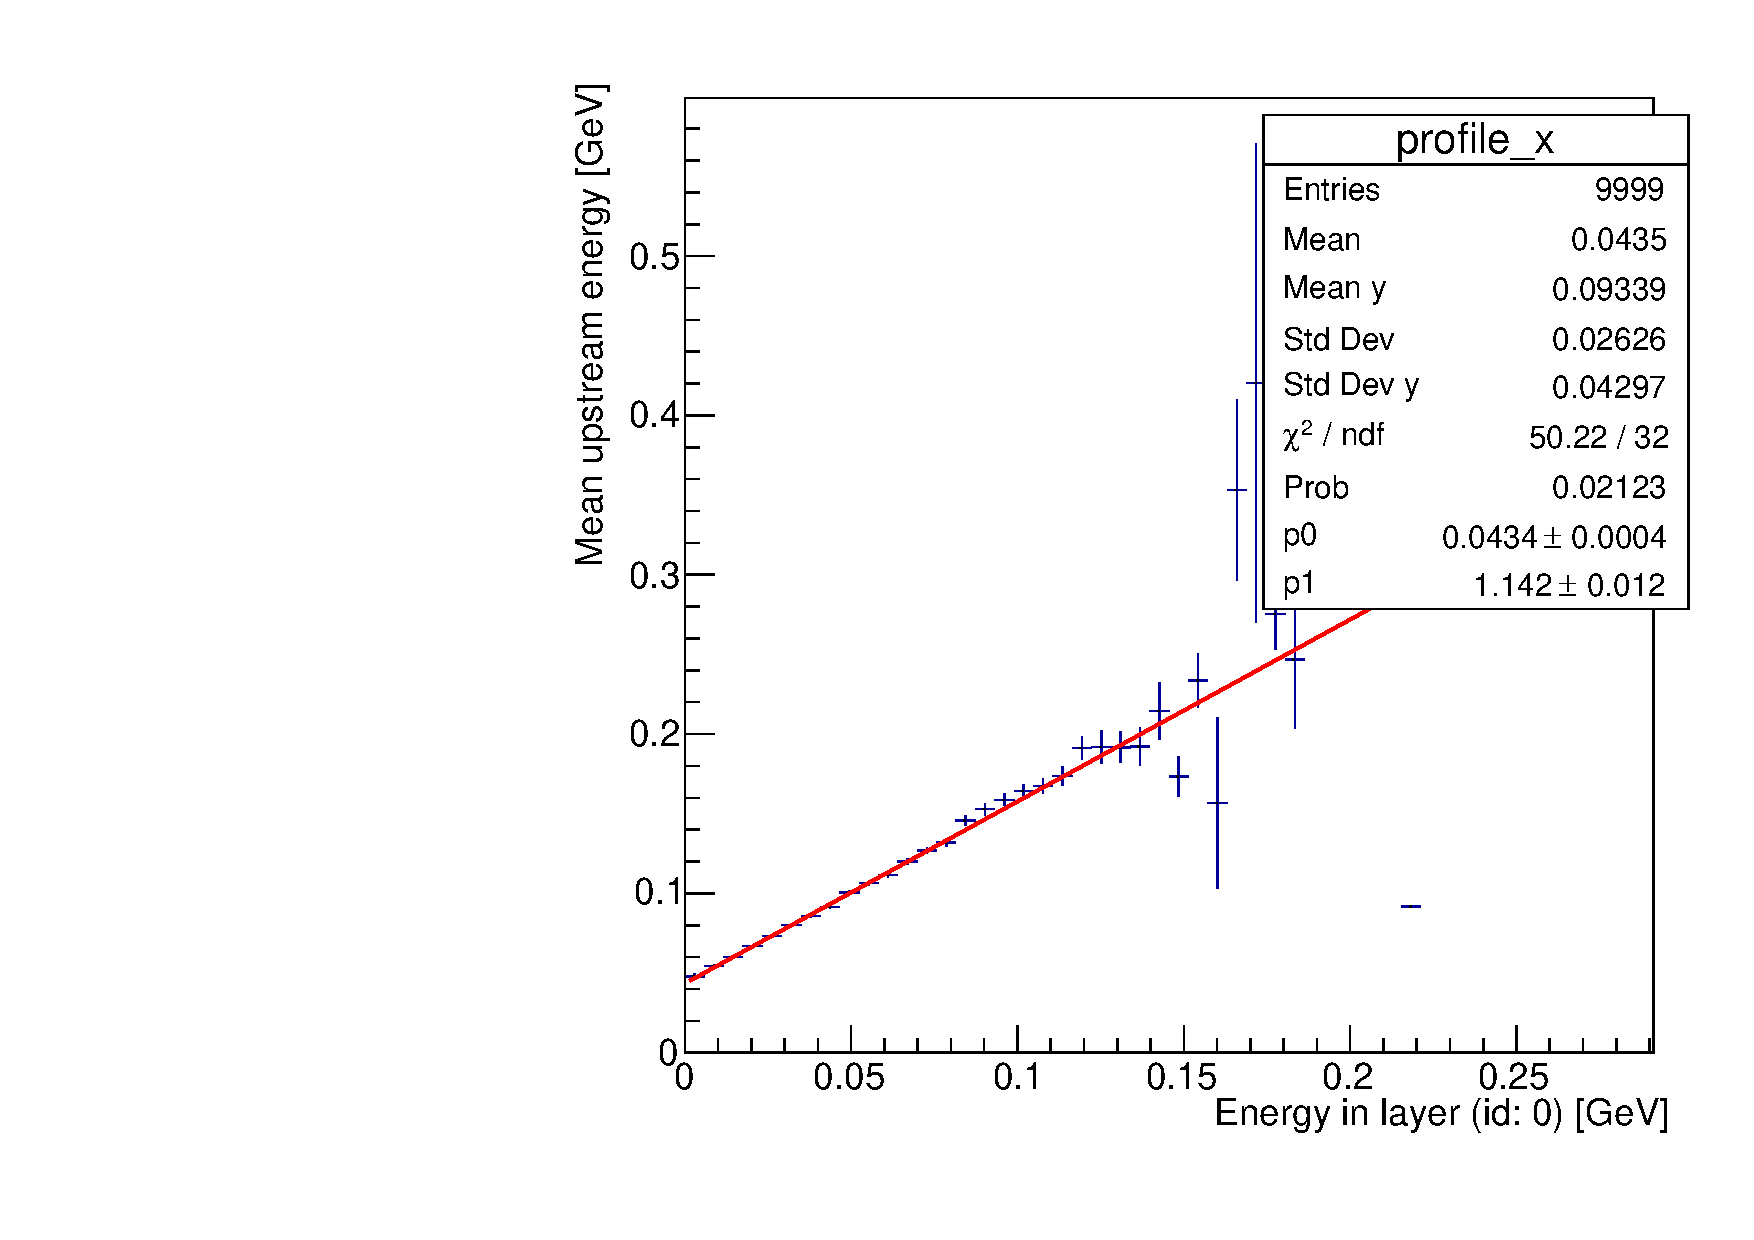
\includegraphics[width=0.39\linewidth]{figures/momentum_id0/profile_upstream_vs_first_layer_90deg_50GeV.pdf} \\
  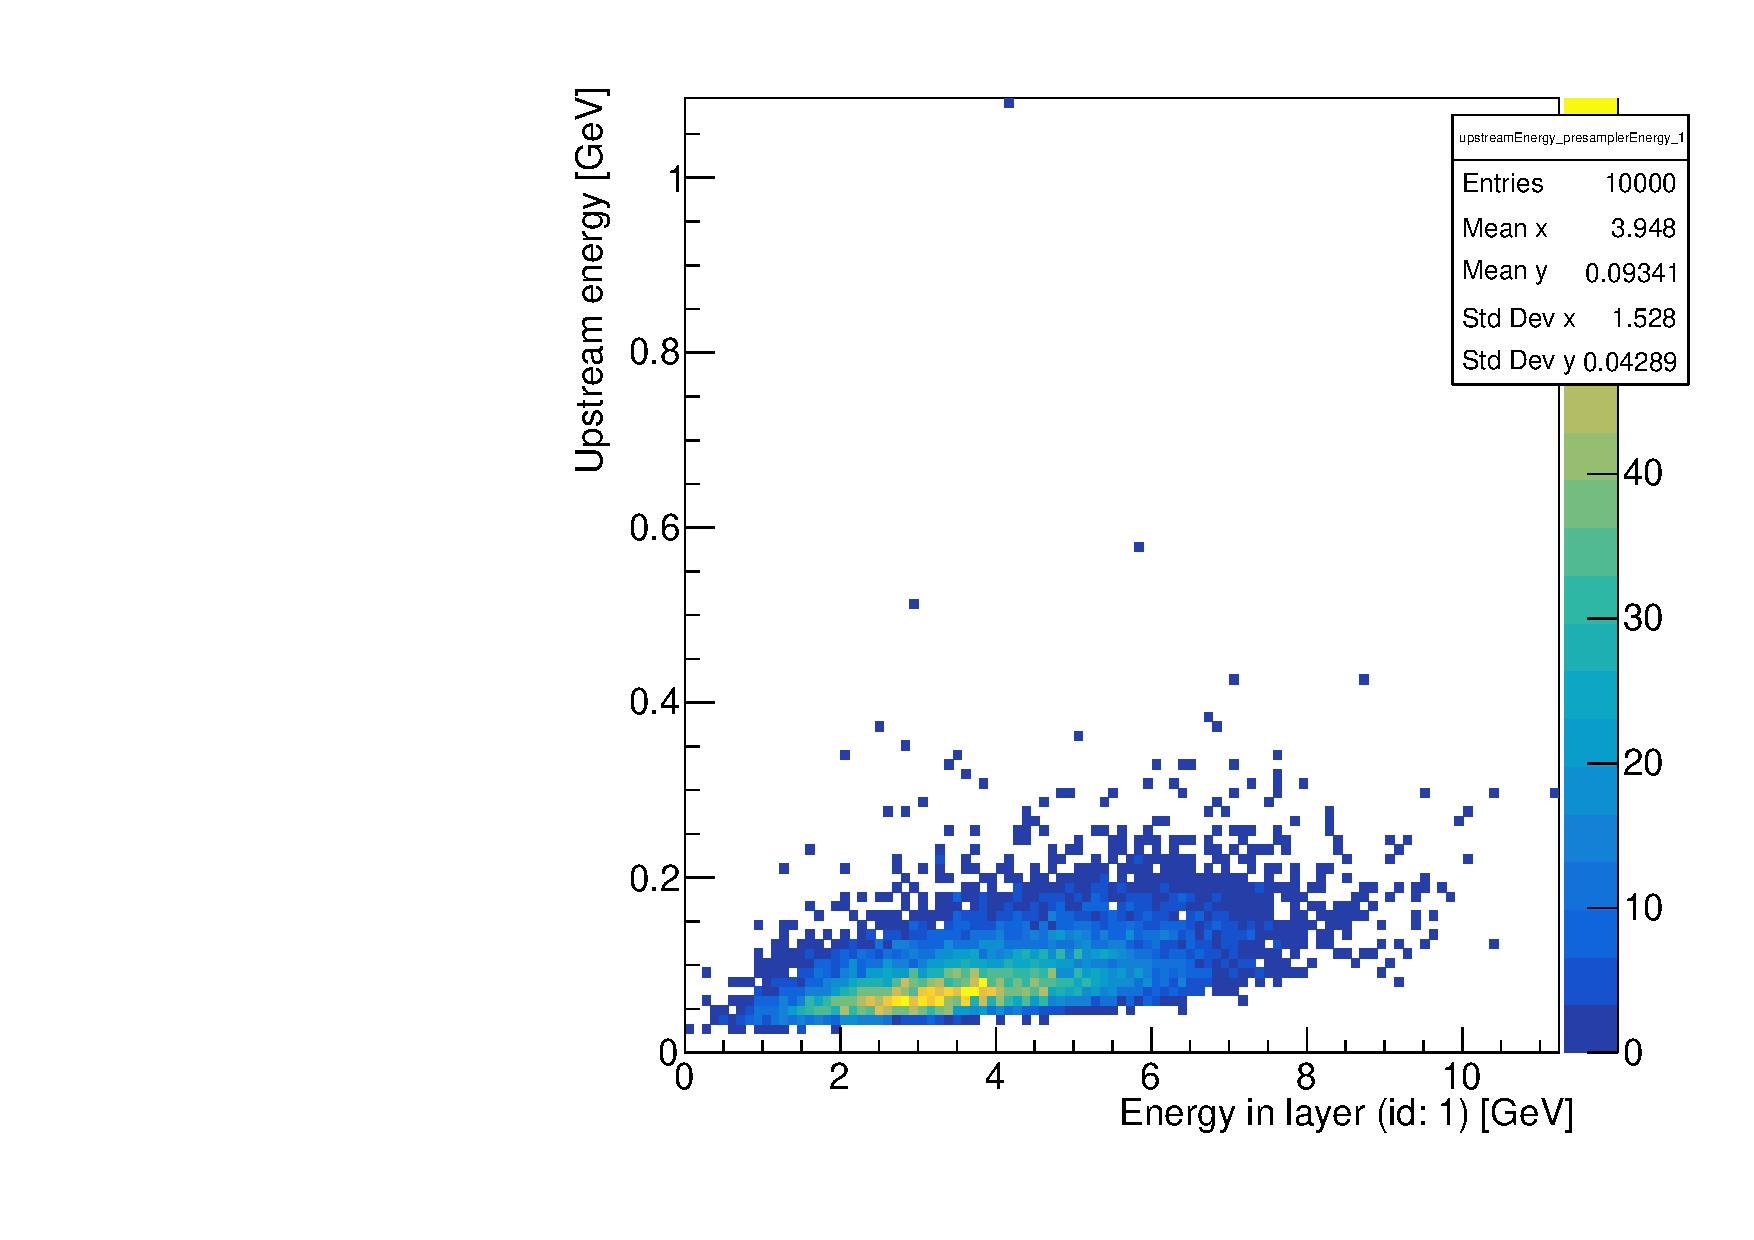
\includegraphics[width=0.39\linewidth]{figures/momentum_id1/hist_upstream_vs_first_layer_90deg_50GeV.pdf}
  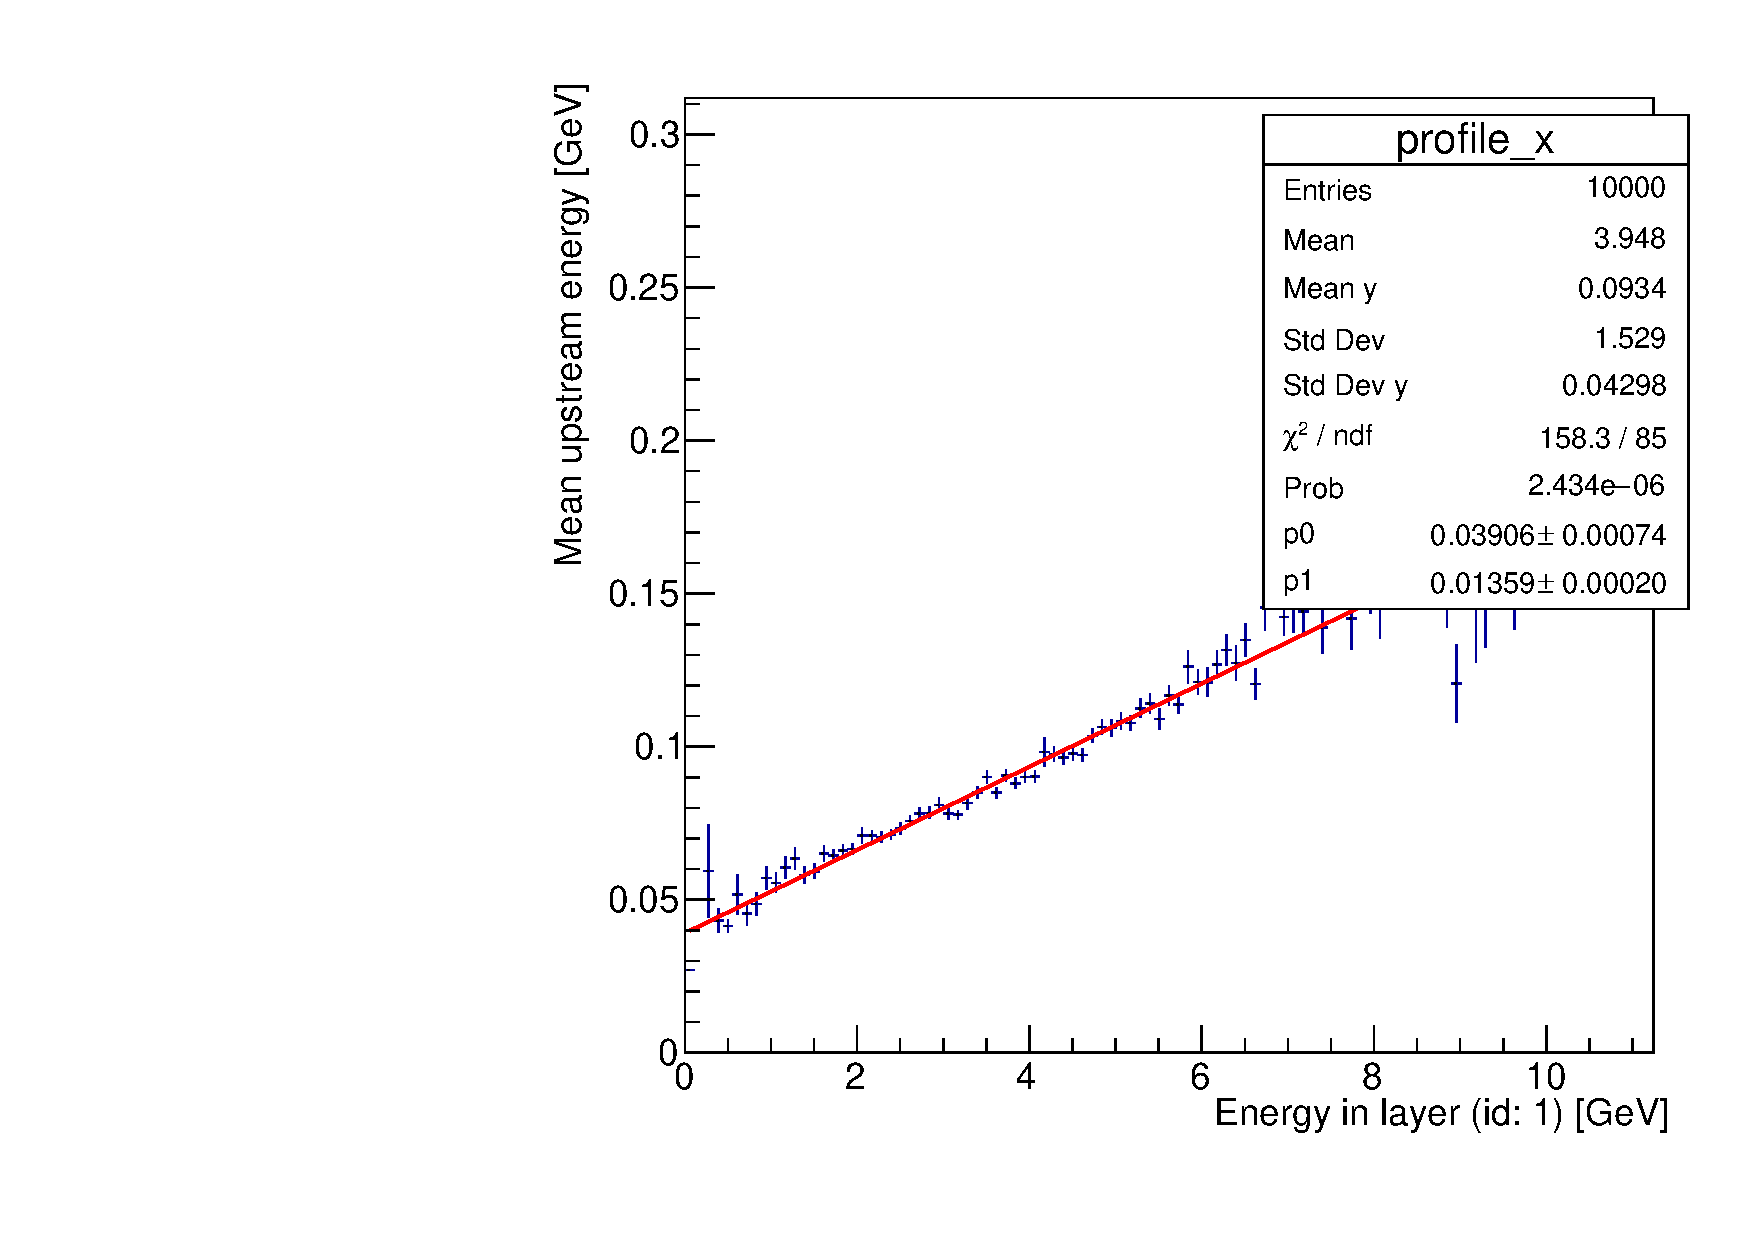
\includegraphics[width=0.39\linewidth]{figures/momentum_id1/profile_upstream_vs_first_layer_90deg_50GeV.pdf}
\end{frame}

\begin{frame}
  \frametitle{At 75 GeV}

  \centering
  \includegraphics[width=0.39\linewidth]{figures/momentum_id0/hist_upstream_vs_first_layer_90deg_75GeV.pdf}
  \includegraphics[width=0.39\linewidth]{figures/momentum_id0/profile_upstream_vs_first_layer_90deg_75GeV.pdf} \\
  \includegraphics[width=0.39\linewidth]{figures/momentum_id1/hist_upstream_vs_first_layer_90deg_75GeV.pdf}
  \includegraphics[width=0.39\linewidth]{figures/momentum_id1/profile_upstream_vs_first_layer_90deg_75GeV.pdf}
\end{frame}

\begin{frame}
  \frametitle{At 100 GeV}

  \centering
  \includegraphics[width=0.39\linewidth]{figures/momentum_id0/hist_upstream_vs_first_layer_90deg_100GeV.pdf}
  \includegraphics[width=0.39\linewidth]{figures/momentum_id0/profile_upstream_vs_first_layer_90deg_100GeV.pdf} \\
  \includegraphics[width=0.39\linewidth]{figures/momentum_id1/hist_upstream_vs_first_layer_90deg_100GeV.pdf}
  \includegraphics[width=0.39\linewidth]{figures/momentum_id1/profile_upstream_vs_first_layer_90deg_100GeV.pdf}
\end{frame}

\begin{frame}
  \frametitle{At 125 GeV}

  \centering
  \includegraphics[width=0.39\linewidth]{figures/momentum_id0/hist_upstream_vs_first_layer_90deg_125GeV.pdf}
  \includegraphics[width=0.39\linewidth]{figures/momentum_id0/profile_upstream_vs_first_layer_90deg_125GeV.pdf} \\
  \includegraphics[width=0.39\linewidth]{figures/momentum_id1/hist_upstream_vs_first_layer_90deg_125GeV.pdf}
  \includegraphics[width=0.39\linewidth]{figures/momentum_id1/profile_upstream_vs_first_layer_90deg_125GeV.pdf}
\end{frame}

\begin{frame}
  \frametitle{At 150 GeV}

  \centering
  \includegraphics[width=0.39\linewidth]{figures/momentum_id0/hist_upstream_vs_first_layer_90deg_150GeV.pdf}
  \includegraphics[width=0.39\linewidth]{figures/momentum_id0/profile_upstream_vs_first_layer_90deg_150GeV.pdf} \\
  \includegraphics[width=0.39\linewidth]{figures/momentum_id1/hist_upstream_vs_first_layer_90deg_150GeV.pdf}
  \includegraphics[width=0.39\linewidth]{figures/momentum_id1/profile_upstream_vs_first_layer_90deg_150GeV.pdf}
\end{frame}

\begin{frame}
  \frametitle{At 200 GeV}

  \centering
  \includegraphics[width=0.39\linewidth]{figures/momentum_id0/hist_upstream_vs_first_layer_90deg_200GeV.pdf}
  \includegraphics[width=0.39\linewidth]{figures/momentum_id0/profile_upstream_vs_first_layer_90deg_200GeV.pdf} \\
  \includegraphics[width=0.39\linewidth]{figures/momentum_id1/hist_upstream_vs_first_layer_90deg_200GeV.pdf}
  \includegraphics[width=0.39\linewidth]{figures/momentum_id1/profile_upstream_vs_first_layer_90deg_200GeV.pdf}
\end{frame}


% ---------------------------------------------------------------------------- %
\section{Angle $\theta$ dependence}

\begin{frame}
  \frametitle{FCC-ee IDEA-LAr Upstream Correction}

  \begin{center}
    $\theta$ dependence, Layer \redtext{ID:\@ 0}
  \end{center}

  \includegraphics[width=0.49\linewidth]{figures/theta_id0/graph_upstream_corr_theta_param0.pdf}
  \includegraphics[width=0.49\linewidth]{figures/theta_id0/graph_upstream_corr_theta_param1.pdf}
\end{frame}

\begin{frame}
  \frametitle{FCC-ee IDEA-LAr Upstream Correction}

  \begin{center}
    $\theta$ dependence, Layer \redtext{ID:\@ 1}
  \end{center}

  \includegraphics[width=0.49\linewidth]{figures/theta_id1/graph_upstream_corr_theta_param0.pdf}
  \includegraphics[width=0.49\linewidth]{figures/theta_id1/graph_upstream_corr_theta_param1.pdf}
\end{frame}

\begin{frame}
  \frametitle{At 90 deg}
  \centering
  \includegraphics[width=0.39\linewidth]{figures/theta_id0/hist_upstream_vs_first_layer_90deg_50GeV.pdf}
  \includegraphics[width=0.39\linewidth]{figures/theta_id0/profile_upstream_vs_first_layer_90deg_50GeV.pdf} \\
  \includegraphics[width=0.39\linewidth]{figures/theta_id1/hist_upstream_vs_first_layer_90deg_50GeV.pdf}
  \includegraphics[width=0.39\linewidth]{figures/theta_id1/profile_upstream_vs_first_layer_90deg_50GeV.pdf}
\end{frame}

\begin{frame}
  \frametitle{At 85 deg}
  \centering
  \includegraphics[width=0.39\linewidth]{figures/theta_id0/hist_upstream_vs_first_layer_85deg_50GeV.pdf}
  \includegraphics[width=0.39\linewidth]{figures/theta_id0/profile_upstream_vs_first_layer_85deg_50GeV.pdf} \\
  \includegraphics[width=0.39\linewidth]{figures/theta_id1/hist_upstream_vs_first_layer_85deg_50GeV.pdf}
  \includegraphics[width=0.39\linewidth]{figures/theta_id1/profile_upstream_vs_first_layer_85deg_50GeV.pdf}
\end{frame}

\begin{frame}
  \frametitle{At 80 deg}
  \centering
  \includegraphics[width=0.39\linewidth]{figures/theta_id0/hist_upstream_vs_first_layer_80deg_50GeV.pdf}
  \includegraphics[width=0.39\linewidth]{figures/theta_id0/profile_upstream_vs_first_layer_80deg_50GeV.pdf} \\
  \includegraphics[width=0.39\linewidth]{figures/theta_id1/hist_upstream_vs_first_layer_80deg_50GeV.pdf}
  \includegraphics[width=0.39\linewidth]{figures/theta_id1/profile_upstream_vs_first_layer_80deg_50GeV.pdf}
\end{frame}

\begin{frame}
  \frametitle{At 75 deg}
  \centering
  \includegraphics[width=0.39\linewidth]{figures/theta_id0/hist_upstream_vs_first_layer_75deg_50GeV.pdf}
  \includegraphics[width=0.39\linewidth]{figures/theta_id0/profile_upstream_vs_first_layer_75deg_50GeV.pdf} \\
  \includegraphics[width=0.39\linewidth]{figures/theta_id1/hist_upstream_vs_first_layer_75deg_50GeV.pdf}
  \includegraphics[width=0.39\linewidth]{figures/theta_id1/profile_upstream_vs_first_layer_75deg_50GeV.pdf}
\end{frame}

\begin{frame}
  \frametitle{At 70 deg}
  \centering
  \includegraphics[width=0.39\linewidth]{figures/theta_id0/hist_upstream_vs_first_layer_70deg_50GeV.pdf}
  \includegraphics[width=0.39\linewidth]{figures/theta_id0/profile_upstream_vs_first_layer_70deg_50GeV.pdf} \\
  \includegraphics[width=0.39\linewidth]{figures/theta_id1/hist_upstream_vs_first_layer_70deg_50GeV.pdf}
  \includegraphics[width=0.39\linewidth]{figures/theta_id1/profile_upstream_vs_first_layer_70deg_50GeV.pdf}
\end{frame}

\begin{frame}
  \frametitle{At 65 deg}
  \centering
  \includegraphics[width=0.39\linewidth]{figures/theta_id0/hist_upstream_vs_first_layer_65deg_50GeV.pdf}
  \includegraphics[width=0.39\linewidth]{figures/theta_id0/profile_upstream_vs_first_layer_65deg_50GeV.pdf} \\
  \includegraphics[width=0.39\linewidth]{figures/theta_id1/hist_upstream_vs_first_layer_65deg_50GeV.pdf}
  \includegraphics[width=0.39\linewidth]{figures/theta_id1/profile_upstream_vs_first_layer_65deg_50GeV.pdf}
\end{frame}

\begin{frame}
  \frametitle{At 60 deg}
  \centering
  \includegraphics[width=0.39\linewidth]{figures/theta_id0/hist_upstream_vs_first_layer_60deg_50GeV.pdf}
  \includegraphics[width=0.39\linewidth]{figures/theta_id0/profile_upstream_vs_first_layer_60deg_50GeV.pdf} \\
  \includegraphics[width=0.39\linewidth]{figures/theta_id1/hist_upstream_vs_first_layer_60deg_50GeV.pdf}
  \includegraphics[width=0.39\linewidth]{figures/theta_id1/profile_upstream_vs_first_layer_60deg_50GeV.pdf}
\end{frame}

\begin{frame}
  \frametitle{At 55 deg}
  \centering
  \includegraphics[width=0.39\linewidth]{figures/theta_id0/hist_upstream_vs_first_layer_55deg_50GeV.pdf}
  \includegraphics[width=0.39\linewidth]{figures/theta_id0/profile_upstream_vs_first_layer_55deg_50GeV.pdf} \\
  \includegraphics[width=0.39\linewidth]{figures/theta_id1/hist_upstream_vs_first_layer_55deg_50GeV.pdf}
  \includegraphics[width=0.39\linewidth]{figures/theta_id1/profile_upstream_vs_first_layer_55deg_50GeV.pdf}
\end{frame}

\begin{frame}
  \frametitle{At 50 deg}
  \centering
  \includegraphics[width=0.39\linewidth]{figures/theta_id0/hist_upstream_vs_first_layer_50deg_50GeV.pdf}
  \includegraphics[width=0.39\linewidth]{figures/theta_id0/profile_upstream_vs_first_layer_50deg_50GeV.pdf} \\
  \includegraphics[width=0.39\linewidth]{figures/theta_id1/hist_upstream_vs_first_layer_50deg_50GeV.pdf}
  \includegraphics[width=0.39\linewidth]{figures/theta_id1/profile_upstream_vs_first_layer_50deg_50GeV.pdf}
\end{frame}

\begin{frame}
  \frametitle{At 45 deg}
  \centering
  \includegraphics[width=0.39\linewidth]{figures/theta_id0/hist_upstream_vs_first_layer_45deg_50GeV.pdf}
  \includegraphics[width=0.39\linewidth]{figures/theta_id0/profile_upstream_vs_first_layer_45deg_50GeV.pdf} \\
  \includegraphics[width=0.39\linewidth]{figures/theta_id1/hist_upstream_vs_first_layer_45deg_50GeV.pdf}
  \includegraphics[width=0.39\linewidth]{figures/theta_id1/profile_upstream_vs_first_layer_45deg_50GeV.pdf}
\end{frame}

\backupend{}

\end{document}
